%definira klasu dokumenta 
\documentclass[12pt]{report} 



%prostor izmedu naredbi \documentclass i \begin{document} se zove uvod. U njemu se nalaze naredbe koje se odnose na cijeli dokument

%osnovni LaTex ne može riješiti sve probleme, pa se koriste različiti paketi koji olakšavaju izradu željenog dokumenta
\usepackage[croatian]{babel} 
\usepackage{amssymb}
\usepackage{amsmath}
\usepackage{txfonts}
\usepackage{mathdots}
\usepackage{titlesec}
\usepackage{array}
\usepackage{lastpage}
\usepackage{etoolbox}
\usepackage{tabularray}
\usepackage{color, colortbl}
\usepackage{adjustbox}
\usepackage{geometry}
\usepackage[classicReIm]{kpfonts}
\usepackage{hyperref}
\usepackage{fancyhdr}
\usepackage{graphicx}
\usepackage{flafter}

\usepackage{float}
\usepackage{setspace}
\restylefloat{table}


\makeatletter
\newcommand{\setword}[2]{%
	\phantomsection
	%\graphicspath{ {./} }
	#1\def\@currentlabel{\unexpanded{#1}}\label{#2}%
}
\makeatother


\patchcmd{\chapter}{\thispagestyle{plain}}{\thispagestyle{fancy}}{}{} %redefiniranje stila stranice u paketu fancyhdr

%oblik naslova poglavlja
\titleformat{\chapter}{\normalfont\huge\bfseries}{\thechapter.}{20pt}{\Huge}
\titlespacing{\chapter}{0pt}{0pt}{40pt}


\linespread{1.3} %razmak između redaka

\geometry{a4paper, left=1in, top=1in,}  %oblik stranice

\hypersetup{ colorlinks, citecolor=black, filecolor=black, linkcolor=black,	urlcolor=black }   %izgled poveznice


%prored smanjen između redaka u nabrajanjima i popisima
\newenvironment{packed_enum}{
	\begin{enumerate}
		\setlength{\itemsep}{0pt}
		\setlength{\parskip}{0pt}
		\setlength{\parsep}{0pt}
	}{\end{enumerate}}

\newenvironment{packed_item}{
	\begin{itemize}
		\setlength{\itemsep}{0pt}
		\setlength{\parskip}{0pt}
		\setlength{\parsep}{0pt}
	}{\end{itemize}}




%boja za privatni i udaljeni kljuc u tablicama
\definecolor{LightBlue}{rgb}{0.9,0.9,1}
\definecolor{LightGreen}{rgb}{0.9,1,0.9}

%Promjena teksta za dugačke tablice
\DefTblrTemplate{contfoot-text}{normal}{Nastavljeno na idućoj stranici}
\SetTblrTemplate{contfoot-text}{normal}
\DefTblrTemplate{conthead-text}{normal}{(Nastavljeno)}
\SetTblrTemplate{conthead-text}{normal}
\DefTblrTemplate{middlehead,lasthead}{normal}{Nastavljeno od prethodne stranice}
\SetTblrTemplate{middlehead,lasthead}{normal}

%podesavanje zaglavlja i podnožja

\pagestyle{fancy}
\lhead{Programsko inženjerstvo}
\rhead{SatCom}
\lfoot{ExpressoDepresso}
\cfoot{stranica \thepage/\pageref{LastPage}}
\rfoot{\today}
\renewcommand{\headrulewidth}{0.2pt}
\renewcommand{\footrulewidth}{0.2pt}


\begin{document} 
	
	
	
	\begin{titlepage}
		\begin{center}
			\vspace*{\stretch{1.0}} %u kombinaciji s ostalim \vspace naredbama definira razmak između redaka teksta
			\LARGE Programsko inženjerstvo\\
			\large Ak. god. 2022./2023.\\
			
			\vspace*{\stretch{3.0}}
			
			\huge SatCom\\
			\Large Dokumentacija, Rev.  2.0\\
			
			\vspace*{\stretch{12.0}}
			\normalsize
			Grupa: ExpressoDepresso\\
			Voditelj: Mihael Pristav\\
			
			
			\vspace*{\stretch{1.0}}
			Datum predaje: 13.1.2023.\\
	
			\vspace*{\stretch{4.0}}
			
			Nastavnik: Goran Rajić\\
		
		\end{center}

	
	\end{titlepage}

	
	\tableofcontents


	\chapter{Dnevnik promjena dokumentacije}
			
		\begin{longtblr}[
				label=none
			]{
				width = \textwidth, 
				colspec={|X[1.5,m]|X[10,m]|X[5,m]|X[3,m]|}, 
				cell{1-46}{1,3-4}={c,c},
				rowhead = 1
			}
			\hline
			\textbf{Rev.}	& \textbf{Opis promjene/dodatka} & \textbf{Autori} & \textbf{Datum}\\[3pt] \hline
			0.1 & Napravljen predložak.\newline Popunjeni osnovni podaci.\newline Osvježen dnevnik sastajanja	& Mihael Pristav & 23.10.2022. 		\\ \hline 
			0.1.1 &Osvježen dnevnik sastajanja  & Mihael Pristav &  25.10.2022.	\\[3pt] \hline
			0.1.2 &Osvježen dnevnik sastajanja  & Mihael Pristav &  26.10.2022.	\\[3pt] \hline 
			0.2 & Započeta cjelina Arhitektura i \newline dizajn. \newline Opis tablica baze podataka &  Marta Vidas\newline Ivan Žgela & 28.10.2022. \\[3pt] \hline 
   			0.3 &Započeta cjelina Opis projektnog zadatka & Maria Carmen \newline Belušić Gonzalez & 30.10.2022. \\[3pt] \hline 
			0.3.1 &Osvježen dnevnik sastajanja  & Mihael Pristav &  30.10.2022.	\\[3pt] \hline
            0.3.2 &Osvježen dnevnik sastajanja & Ivan Žgela & 31.10.2022  \\[3pt] \hline
			0.4 &Započeta cjelina funkcionalni \newline zahtjevi &  Leona Salihović & 1.11.2022.  \\[3pt] \hline 
			0.4.1 & Osvježen dnevnik sastajanja \newline Ispravljene prijašnje greške u\newline dokumentaciji  & Mihael Pristav & 2.11.2022.  \\[3pt] \hline 
			0.4.2 & Dodan sadržaj u cjelinu\newline funkcionalni zahtjevi  & Leona Salihović &  3.11.2022. \\[3pt] \hline 
			0.4.3 & Promijenjen sadržaj u cjelini\newline funkcionalni zahtjevi & Leona Salihović & 3.11.2022.   \\[3pt] \hline
			0.4.4 & Osvježen dnevnik sastajanja \newline Ispravljene prijašnje greške u\newline dokumentaciji
			\newline Dodani dijagrami obrazaca uporabe  & Mihael Pristav & 3.11.2022.  \\[3pt] \hline 
			0.4.5 & Dorađen opis postojećih tablica baze podataka i dodane nove & Marta Vidas & 7.11.2022.  \\[3pt] \hline  
			0.4.6 & Upisano pola obrazaca uporabe\newline Dopunjena tablica uloženih sati\newline Popravljeno uređenje dijelova\newline dokumentacije\ & Mihael Pristav\newline Marta Vidas & 7.11.2022.  \\[3pt] \hline 
			0.4.7 & Osviježen opis baze podataka & Mihael Pristav & 8.11.2022.  \\[3pt] \hline
			0.4.8 & Dodani obrasci uporabe & Mihael Pristav & 9.11.2022.  \\[3pt] \hline
			0.5 & Osvježeni obrasci uporabe\newline Osviježen dnevnik sastajanja\newline Dodani prvi sekvencijski dijagrami
			 \newline Ispravljene primjećene greške u\newline tekstu \newline Ispravljena neka upozorenja i\newline pogreške u Latex sintaksi  & Mihael Pristav & 11.11.2022.  \\[3pt] \hline
			 0.5.1 & Osvježeni obrasci uporabe\newline Podešeni sekvencijski diagrami za \newline bolju preglednost i čitljivost\newline Dodani opisi sekvencijskih dijagrama\newline Podešena custom naredba za referenciranje i njezino korištenje u dokumentaciji
			   & Mihael Pristav & 12.11.2022.  \\[3pt] \hline
			0.5.2 & Manje promjene u oblikovanju stranica\newline Popravljen 2. sekvencijski dijagram   & Mihael Pristav & 13.11.2022.  \\[3pt] \hline 
			0.5.3 & Dopunjeni funkcionalni zahtjevi\newline običnog uporabnog korisnika\newline Osvježen opis i atributi baze\newline Dodani obrasci uporabe & Mihael Pristav & 14.11.2022.  \\[3pt] \hline
			 
				0.5.4 & Osvježen dijagram baze\newline Dodani obrasci uporabe & Mihael Pristav & 15.11.2022.  \\[3pt] \hline
            0.5.5 & Dodavanje obrazaca uporabe za satelite (prikaz liste satelita, edit, delete i dodavanje novog satelita)\newline Dodani sati provedeni na kodiranje aplikacije & Ivan Žgela & 15.11.2022.  \\[3pt] \hline
             0.5.6 & Dodavanje obrazaca uporabe za\newline prikaz informacija satelita\newline Ispravljene pogrešno podešene\newline reference\newline Ispravljene manje greške u \newline oblikovanju\newline Osvježeni opisi obrazaca uporabe u odnosu na novi dijagram obrazaca uporabe  & Mihael Pristav & 15.11.2022.  \\[3pt] \hline
             0.5.7 &  Dodavanje obrazaca uporabe za transmitere (prikaz liste transmitera, edit, delete i dodavanje novog transmitera) & Leona Salihović & 15.11.2022.  \\[3pt] \hline
			0.5.8 &Dodani dijagrami razreda i njihovi opisi\newline Proširen opis projektnog zadatka\newline ispravljene greške u  svom\newline dosadašnjem tekstu\newline popravljeno formatiranje teksta u dokumentu & Maria Carmen\newline Belušić Gonzales\newline Leticija Crnković\newline Mihael Pristav\newline Marta Vidas &17.11.2022.  \\[3pt] \hline 
			\textbf{1.0}& Dodavanje dosadašnje literature\newline Završna kontrola teksta& Mihael Pristav&18.11.2022.\\[3pt]\hline
			1.0.1 &Ispravljene manje greške u opisu baze podataka &Mihael Pristav & 6.12.2022.  \\[3pt] \hline 
			1.0.2 &Dopunjeni ostali zahtjevi &Mihael Pristav & 9.1.2023.  \\[3pt] \hline 
			1.0.3 &Usklađen opis zadatka s trenutačnim stanjem aplikacije &Mihael Pristav & 9.1.2023.  \\[3pt] \hline
			1.0.4 &Započeta cjelina Korištene tehnologije i alati &Leona Salihović & 9.1.2023.  \\[3pt] \hline
			1.0.5 &Promjene u cjelini Korištene tehnologije i alati &Leona Salihović & 10.1.2023.  \\[3pt] \hline 	
			1.1.0 &Započeta cjelina Zaključak &Leona Salihović & 11.1.2023.  \\[3pt] \hline 	
			1.1.1 &Dovršena Aktualizacija obrazaca uporabe & Mihael Pristav & 11.1.2023.  \\[3pt] \hline
			1.1.2 &Promjene u cjelinama Zaključak i Korištene tehnologije i alati & Leona Salihović & 12.1.2023.  \\[3pt] \hline	
			1.2.0 &Započeta cjelina Dijagram razmještaja& Leona Salihović & 12.1.2023.  \\[3pt] \hline		
			1.2.1 &Dodan dijagram razmještaja& Leona Salihović & 12.1.2023.\\[3pt] \hline
			1.2.2 &Ispravljenenovo nastale pogreške kod referenciranja i foramtiranja dokumenta& Mihael Pristav & 12.1.2023.\\[3pt] \hline
				1.3.0 &Dodana cjelina ispitivanje komponenti& Marta Vidas & 12.1.2023.\\[3pt] \hline
			1.3.1 &Osvježeni dijagrami razreda& Leticija Crnković & 12.1.2023.\\[3pt] \hline
			1.3.2 &Osvježeni sekvencijski dijagrami \newline 
				Ispravljeno referenciranje slika&Mihael Pristav & 13.1.2023.\\[3pt] \hline
            1.4.0 & Dodana cjelina za Dijagram komponenti\newline
             Dopunjen Dijagram aktivnosti & Dalen Grdić & 13.1.2023.\\[3pt] \hline
            1.4.1 & Dodana cjelina Ispitivanje sustava & Maria Carmen Belušić Gonzalez & 13.1.2023.\\[3pt] \hline
            1.5.0 & Dovršene upute za puštanje u pogon & Leticija Crnković & 13.1.2023.\\[3pt] \hline
            \textbf{2.0}& Dodavanje grafova aktivnosti na gitLabu\newline Završna kontrola teksta& Mihael Pristav&13.1.2023.\\[3pt]\hline
	
		
		\end{longtblr}
	\chapter{Opis projektnog zadatka}
		
		
        {   Cilj ovog projekta je izrada programske potpore za web aplikaciju \textit{SatCom} koja svojim korisnicima omogućuje olakšan i intuitivan način komunikacije sa simuliranim satelitima uz pomoć \textit{SatNOGS} mreže. Zainteresirani korisnici mogu biti dio istraživačke, znanstvene i akademske zajednice ili bilo koja skupina zainteresirana za testiranje komunikacije sa satelitima.} \par
        {   Zbog velike koristi satelita, njihove široke primjene i povećane troškovne dostupnosti, u posljednjem desetljeću pojavljuje se sve veći broj satelita otvorenog, akademskog tipa, a uz to i pitanje ostvarivanja komunikacije s njima. Općenito, sateliti komuniciraju koristeći se radio komunikacijskim vezama za razašiljanje poruka prema zemaljskim stanicama, nakon čega stanice prime poruku i obrađuju informacije koje poruka sadrži (podatci o satelitu, lokacija satelita, satelitske slike i sl).} \par
        { U aplikaciji postoje tri uloge:
        \begin{packed_item}
            \item običan uporabni korisnik,
            \item administrator aplikacije,
            \item administrator satelita.
        \end{packed_item}
        {Funkcionalnosti kojima može pristupiti \textit{običan uporabni korisnik} mogu pristupati i korisnici s preostalim ulogama. Razlika je što korisnici s ulogama \textit{administrator aplikacije} i \textit{administrator satelita} imaju pristup dodatnim funkcionalnostima.} \par
        
        {Registraciju novih korisnika može obaviti samo korisnik s ulogom \textit{administrator aplikacije} klikom na gumb \textit{Add New User} na stranici \textit{Users}. Pri registriranju novog korisnika potrebno je upisati e-mail adresu, korisničko ime, lozinku i dodijeliti mu jednu od uloga.} \par
        {Osim registracije korisnika, korisnik s ulogom \textit{administrator aplikacije} može pregledati sve korisnike aplikacije i brisati ih putem stranice \textit{Users} na kojoj se prikazuje lista svih korisnika aplikacije u tabličnom prikazu. Svaki redak tablice sadrži ikonu za brisanje odabranog korisnika.} \par

        {Neregistrirani korisnici ne mogu pristupiti funkcionalnostima aplikacije.} \par
        
        {Registriranom i prijavljenom korisniku omogućene su razne aktivnosti u aplikaciji. Korisnik može pristupiti početnoj stranici na kojoj je opisan cilj SatCom projekta i objašnjenje osnovnih pojmova koji se koriste u aplikaciji: 
        \begin{packed_item}
            \item satelit,
            \item zemaljska stanica,
            \item komunikacijski link, 
            \item transmiter.
        \end{packed_item}
        Korisnik inicijalizira postupak slanja poruka na satelit klikom na gumb\newline \textit{Send message} koji se nalazi u zaglavlju i na početnoj stranici. \par
        
        {   Stranica \textit{Send Message} sadrži popis svih satelita i njihovih atributa u tabličnom prikazu i omogućuje korisniku pretraživanje satelita putem tražilice na vrhu tablice. Korisnik odabire satelit s kojim želi ostvariti komunikaciju klikom na redak u tablici. Nakon odabira stanice, korisniku se na vrhu stranice prikaže odabrani satelit, njegove informacije i informacije o njegovim transmiterima, a ispod se nalazi lista svih kompatibilnih komunikacijskih linkova od kojih mora odabrati jedan. Potom korisnik mora odabrati želi li odabir zemaljske stanice ostvariti automatski ili manualno. Automatski odabir podrazumijeva da se o odabiru zemaljske stanice brine sustav. Kod manualnog, korisniku se prepušta odabir jedne od kompatibilnih zemaljskih stanica. U zadnjem koraku korisnik unosi poruku koju želi poslati i zatim čeka odgovor od satelita.} \par
        
        {Običan korisnik također može pristupiti svom profilu na stranici \textit{My Profile} koja sadrži korisnikove osobne podatke i gumbove kojima pristupa uređivanju profila te pregledu povijesti poslanih zahtjeva komunikacije sa satelitima. Korisnik može mijenjati korisničko ime i lozinku klikom na gumb \textit{Edit profile}. Pregled poslanih zahtjeva nalazi se na stranici \textit{Message History}, gdje se korisniku prikazuje zapis satelita s kojima je uspješno komunicirao, kao i svi parametri komunikacije (vrijeme slanja poruke, zemaljska stanica, komunikacijski link te sadržaj poruke i odgovora). Povijest komunikacija može se obrisati klikom na gumb \textit{Erase All}.} \par

        
        {Korisnik s ulogom \textit{administrator satelita} može obavljati razne akcije nad satelitima, komunikacijskim linkovima i transmiterima.} \par
        {Satelitima pristupa putem stranice \textit{Satellites} na kojoj su prikazani svi sateliti i njihovi atributi u tabličnom prikazu. Na toj stranici, administratoru satelita ponuđene su opcije pregleda podataka, dodavanja novih satelita, brisanja i\newline uređivanja satelita. Klikom na redak u tablici, otvara se stranica \textit{Satellite Details}. Na vrhu navedene stranice nalaze se svi atributi odabranog satelita, a ispod lista povezanih transmitera i njihove informacije. Klikom na jedan od transmitera administratoru se prikazuju njegova svojstva i opcije za brisanje i promjenu podataka. Opcijama se pristupa gumbima \textit{Delete transmitter} i \textit{Edit}.
        Formi za dodavanje satelita pristupa se putem gumba \textit{Add New Satellite} gdje se upisuju parametari satelita.
        Brisanje i uređivanje satelita obavlja se klikom na gumbove koji se nalaze na vrhu stranice s podacima o satelitu. Pri uređivanju satelita, administrator satelita može uređivati njegove podatke i dodavati i brisati njegove transmitere.}\par

        {Tabličnom prikazu liste komunikacijskih linkova i njihovih informacija administrator pristupa putem stranice \textit{Links}. Na toj stranici administrator satelita može dodavati nove satelite klikom na gumb \textit{Add New link} čime pristupa formi u koju upisuje podatke novog linka. Klikom na link, prikazuju se informcije o tom linku i opcije za brisanje i uređivanje odabranog linka pomoću gumbova \textit{Delete} i \textit{Edit} koji se nalaze na kraju svakog retka tablice.}


        {Zadnje, administrator može zatražiti prikaz svih transmitera putem stranice \textit{Transmitters}. Tamo može odabrati transmitere, te ih potom brisati i uređivati.}\par


        
        {Bitno je napomenuti da zemaljske stanice ne može niti jedan korisnik mijenjati ili brisati. Sustav se svakog dana u ponoć spaja na \textit{SatNOGS} aplikacijsko sučelje i dohvaća podatke aktivnih zemaljskih stanica.} \par

        {Postoje razne mogućnosti proširenja sadašnjeg rješenja koje bi poboljšale aplikaciju, ali nisu nužne za njenu funkcionalnost:
            \begin{packed_item}
            \item ostvarenje komunikacije sa stvarnim satelitima koji se nalaze na \textit{SatNOGS} mreži,
            \item registriranje vlastitih satelita putem aplikacije na \textit{SatNOGS} mrežu,
            \item omogućavanje korisnicima da satelite na koje često šalju poruke mogu označiti kao \textit{omiljene}, 
            \item implementacija mobilne aplikacije,
            \item slanje zahtjeva administratoru stranice za promjenu e-mail adrese,
            \item slanje zahtjeva za registracijom.
        \end{packed_item}
        }
		
	
	\chapter{Specifikacija programske potpore}
\graphicspath{{./slike/}}		
	\section{Funkcionalni zahtjevi}
			
			\noindent \textbf{Dionici:}
			
			\begin{packed_enum}
				
				\item Vlasnik (naručitelj)
				\item Korisnici
				      \begin{packed_enum}
						
						\item  opći uporabni korisnik 
						\item  administrator aplikacije
						\item administrator satelita
				
					\end{packed_enum}
				\item Razvojni tim
				
			\end{packed_enum}
			
			\noindent \textbf{Aktori i njihovi funkcionalni zahtjevi:}
			
			
			\begin{packed_enum}
				\item  \underbar{Neregistrirani/neprijavljeni korisnik (inicijator) može:}
				
				\begin{packed_enum}
					
					\item se prijaviti u sustav, za što su mu potrebni lozinka (\textit{password}) i korisničko ime (\textit{username})
					
				\end{packed_enum}
			
				\item  \underbar{Obični uporabni korisnik (inicijator) može:}
				
				\begin{packed_enum}
					
					\item se prijaviti u sustav unosom lozinke (\textit{password}) i korisničkog imena (\textit{username}) te promijeniti inicijalo mu dodijeljenu lozinku i korisničko ime
					\item odabrati satelit na kojeg želi poslati poruku i link za komunikaciju 
					\item odlučiti hoće li samostalno odabrati zemeljsku stanicu putem koje se komunicira sa satelitom ili će to sustav napraviti umjesto njega
					\item poslati željeni tekst kao poruku na prethodno odabranu tojku (satelit, link, stanica)
					\item pregledavati i brisati sve poslane poruke i primljene odgovore
					
				\end{packed_enum}
				
				\item  \underbar{Administrator aplikacije (inicijator) može:}
				
				\begin{packed_enum}
					
				    \item kreirati nove korisnike sustava pri čemu im dodijeljue adresu e-pošte (\textit{e-mail}), korisničko ime (\textit{username}), lozinku (\textit{password}) i ulogu (\textit{role})
					\item ostvariti sve funkcionalne zahtjeve običnih uporabnih korisnika
					
				\end{packed_enum}
					\item  \underbar{Administrator satelita (inicijator) može:}
				
				    \begin{packed_enum}
					
				        \item kreirati i izbrisati satelite te promijenjiti njihove parametre
				        \item kreirati i izbrisati linkove te promijenjiti njihove parametre
				        \item kreirati i izbrisati transmitere te promijenjiti njihove parametre
				        \item ostvariti sve funkcionalne zahtjeve običnih uporabnih korisnika
					
				    \end{packed_enum}
				
					\item  \underbar{Baza podataka (sudionik) može:}
				
				\begin{packed_enum}
					
					\item pohraniti sve podatke o korisnicima, njihovim ovlastima i razmijenjenim porukama
					\item pohraniti sve podatke o satelitima, zemaljskim stanicama, linkovima, antenama i transmiterima
					
				\end{packed_enum}
				\item  \underbar{ SatNOGS Network API (sudionik) može:}
				
				\begin{packed_enum}
					
					\item dohvatiti podatke o stanicama i antenama
					
					
				\end{packed_enum}
				\item  \underbar{Satelitte server (sudionik) može:}
			
			\begin{packed_enum}
				
				\item primati poruke koje generira korisnik
				\item odlučiti o prihvaćanju iste poruke
				\item generirati povratnu poruku korisniku
				
				
			\end{packed_enum}
			\end{packed_enum}
			
			\eject 
			
			
				
			\subsection{Obrasci uporabe}

					\noindent \underbar{\textbf{UC1 - Prijava}}
				\begin{packed_item}
					
					\item \textbf{Glavni sudionik: }Neregistrirani korisnik (\textit{guest\_user})
					\item  \textbf{Cilj: }Dobiti pristup korisničkom sučelju
					\item  \textbf{Sudionici: }Baza podataka
				\item \textbf{Preduvjet: }
				\begin{packed_enum}\item Postojanje korisničkog računa u bazi\end{packed_enum}
					\item  \textbf{Opis osnovnog tijeka: }
					
					\item[] \begin{packed_enum}
						
						\item Unos korisničkog imena (\textit{username}) i lozinke (\textit{password})
						\item Sustav potvrđuje ispravnost unesenih podataka
						\item Sustav omogućava pristup korisničkim funkcijama koje definira uloga (\textit{role}) prijavljenog korisnika
						
					\end{packed_enum}
					
					\item  \textbf{Opis mogućih odstupanja: }
					
					\item[] \begin{packed_item}
						
						\item[1] Neispravno korisnicko ime i/ili lozinka
						\item[ ] \begin{packed_enum}
							
							\item[1.1] Sustav obavještava korisnika o neuspjelom upisu i prikazuje\newline prikladnu poruku:  \text "Username or password incorrect"
							
						\end{packed_enum}
						
					\end{packed_item}
				\end{packed_item}
				
				\noindent \underbar{\textbf{UC2 - Pregled osobnih podataka}}
				\begin{packed_item}
					
					\item \textbf{Glavni sudionik: }Korisnik (\textit{user})
					\item  \textbf{Cilj: }Pregledati osobne podatke
					\item  \textbf{Sudionici: }Baza podataka
				\item  \textbf{Preduvjet: }
				\begin{packed_enum}\item Korisnik je prijavljen\end{packed_enum}
					\item  \textbf{Opis osnovnog tijeka: }
					
					\item[] \begin{packed_enum}
					
						\item Korisnik odabire opciju "User details"
						\item Sustav pokazuje osobne podatke korisnika (\textit{username, e-mail} i \textit{ role})
						
					\end{packed_enum}
				\end{packed_item}
				
				\noindent \underbar{\textbf{UC3 - Promjena osobnih podataka}}
				\begin{packed_item}
					
					\item \textbf{Glavni sudionik: }Korisnik (\textit{user})
					\item  \textbf{Cilj: }Promijeniti osobne podatke
					\item  \textbf{Sudionici: }Baza podataka
				\item  \textbf{Preduvjet: }
				\begin{packed_enum}\item Korisnik je prijavljen\end{packed_enum}
					\item  \textbf{Opis osnovnog tijeka: }
					
					\item[] \begin{packed_enum}
						
						\item Korisnik odabere opciju "Edit user details"
						\item Sustav korisniku nudi formu za popunjavanje u kojoj su njegovi trenutni podaci
						\item Korisnik mijenja svoje osobne podatke (\textit{username} i/ili \textit{password})
						\item Korisnik odabere opciju "Save"
						\item Sustav ažurira bazu podataka
						
					\end{packed_enum}
					
					\item  \textbf{Opis mogućih odstupanja: }
					
					\item[] \begin{packed_item}
						
						\item[1] Korisnik promijeni svoje osobne podatke, ali ne odabere opciju "Save"
						\item[ ] \begin{packed_enum}
							
							\item[1.1] Sustav obavještava korisnika da nije spremio podatke prije izlaska iz prozora
							
						\end{packed_enum}
						
						\item[2] Korisnik mijenja \textit{username}, a on je već zauzet
						\item[ ] \begin{packed_enum}
							
							\item[2.1] Sustav obavještava korisnika da je username već zauzet i
							\newline prikazuje prikladnu poruku: "Username already taken"
							
						\end{packed_enum}
						
					\end{packed_item}
				\end{packed_item}
				\noindent \underbar{\textbf{ {\setword{UC4}{Word:UC4}} - Slanje poruke na satelit}}
				\begin{packed_item}
					
					\item \textbf{Glavni sudionik: }Korisnik (\textit{user})
					\item  \textbf{Cilj: }Slanje poruke na odabrani satelit i određivanje parametara
					\item  \textbf{Sudionici: }Baza podataka
					\item  \textbf{Preduvjet: }
					\begin{packed_enum}
					\item Korisnik je prijavljen \item U bazi podataka postoji kompatibilni trio (satelit, link i stanica)	\end{packed_enum}
					\item  \textbf{Opis osnovnog tijeka: }
					
					\item[] \begin{packed_enum}
						
						\item Korisnik odabere opciju za slanje poruke na satelit
						\item Sustav ispisuje listu satelita s nekim njihovim informacijama
						\item Korisnik odabere jedan od satelita
						\item Sustav ispisuje sve podatke o satelitu i njegovim\newline transmiterima
						\item Sustav ispod informacija o satelitu ispisuje listu  kompatibilnih linkova sa svim njihovim informacijama( \textit{frequency}, \textit{mode}, \textit{baud})
						\item Korisnik odabire jedan od linkova
						\item Sustav nudi korisniku opciju da sam odabere željenu stanicu ili da \newline odabir prepusti sustavu
						\item Odabire se kompatibilni satelit ( Vidi \ref{Word:UC5})
						\item {\setword{Sustav vodi korisnika na stranicu s poljem za unošenje teksta poruke}{Word:generiranjem poruke kao što je opisano u UC4}} 
						\item Korisnik unosi poruku i odabire "Send"
						\item Sustav provjerava sa SatNOGS mrežom podudaraju li se naši podaci o \newline odabranoj stanici s trenutnim podacima u njihovoj bazi podataka
						\item Sustav generira sadržaj poruke na temelju vremena slanja, odabranog linka i unesenog teksta
						\item Poruka se označava kao \textit{UPLOAD} i pridružuju joj se parametri komunikacije
						\item Sustav šalje poruku na server(satelit), koji generira povratnu informaciju sličnog formata s oznakom\newline \textit{DOWNLOAD}
						\item Obje poruke se spremaju u bazu podataka s ID oznakom korisnika
						
						
					\end{packed_enum}
					
					\item  \textbf{Opis mogućih odstupanja: }
					
					\item[] \begin{packed_item}
						\item[1] U bazi podataka ne postoji niti jedan satelit
						\item[ ] \begin{packed_enum}
							
							\item[1.1] Sustav obavještava korisnika o nepostojanju satelita
						\end{packed_enum}
					
						\item[2] Poruka poslana na satelit nema definirane sve parametre ili je praznog sadržaja
						\item[ ] \begin{packed_enum}
							
							\item[2.1] Sustav u bazu podataka sprema poruku označenu kao \textit{FAILED UPLOAD}
						\item[2.2] Satelit ne generira povratnu poruku zbog manjka potrebnih informacija o komunikaciji
						\end{packed_enum}	
						\item[3] U bazi podataka ne postoji niti jedan link s odgovarajućim atributima za odabrani satelit
					\item[ ] \begin{packed_enum}
						
						\item[3.1] Sustav obavještava korisnika o nepostojanju odgovarajućeg linka
						\item[3.2] Sustav vraća korisnika na odabir satelita
					\end{packed_enum}		
				\item[4] Sustav je tijekom provjere aktualnosti informacija o stanici, pronašao razliku u podacima bitnim za komunikaciju
				\item[ ] \begin{packed_enum}
					
					\item[4.1] Sustav obavještava korisnika o nemogućnosti slanja poruke odabranim parametrima te ga potiče da pokuša ponovo
					\item[4.2] Sustav osvježava podatke o stanicama i njihovim antenama u bazi podataka
				\end{packed_enum}				
					\end{packed_item}
				\end{packed_item}
			\noindent \underbar{\textbf {\setword{UC5}{Word:UC5} -Biranje stanice}}
			\begin{packed_item}
				
				\item \textbf{Glavni sudionik: }Korisnik (\textit{user})
				\item  \textbf{Cilj: }Odabir zemaljske stanice putem koje se planira poslati poruka
				\item  \textbf{Sudionici: }Baza podataka
				\item  \textbf{Preduvjet: }
				\begin{packed_enum}
					\item Korisnik je prijavljen \item Korisnik je odabrao željeni satelit i link\end{packed_enum}
				\item  \textbf{Opis osnovnog tijeka: }
				
				\item[] \begin{packed_enum}
					
					\item Korisnik ima opciju odabrati "Manual selection" ili "Automatic selection" za odabir stanice
					\item Kod automatskog pretraživanja, sustav odabire stanicu s najvećim brojem obzervacija, koja je kompatibilna s odabranim linkom
					\item Kod ručnog odabira:\begin{itemize}
						\item[a)] Sustav ispisuje listu stanica čije antene podržavaju komunikaciju na način propisan odabranim linkom
						\item[b)] Korisnik odabire stanicu kojom želi poslati poruku
					\end{itemize} 
					\item Nastavljajući proces u \hyperref[Word:generiranjem poruke kao što je opisano u UC4]{UC4} , sustav vodi korisnika na stranicu s poljem za unošenje teksta poruke.
					
				\end{packed_enum}
				
				\item  \textbf{Opis mogućih odstupanja: }
				
				\item[] \begin{packed_item}
				
					\item[1] U bazi podataka ne postoji niti jedna stanica, koja podržava komunikaciju definiranu odabranim linkom
					\item[ ] \begin{packed_enum}
						
						\item[1.1] Sustav obavještava korisnika o nepostojanju adekvatne stanice
						\item[1.2] Sustav vraća korisnika na ponovni izbor satelita( Vidi \ref{Word:UC4})
					\end{packed_enum}
								
					
				\end{packed_item}
			\end{packed_item}
				\noindent \underbar{\textbf{UC6 - Pregled poslanih zahtjeva i rezultata}}
				\begin{packed_item}
					
					\item \textbf{Glavni sudionik: }Korisnik (\textit{user})
					\item  \textbf{Cilj: }Pregled vlastitih komunikacija putem mreže
					\item  \textbf{Sudionici: }Baza podataka
					\item  \textbf{Preduvjet: }
					\begin{packed_enum}\item Korisnik je prijavljen\end{packed_enum}
					\item  \textbf{Opis osnovnog tijeka: }
					
					\item[] \begin{packed_enum}
						
						\item Korisnik odabere opciju "Message history"
						\item Sustav ispisuje tablicu prošlih komunikacija korisnika
						\item U tablici korisnik može vidjeti tekst poruke, vrijeme slanja poruke, smjer komunikacije (\textit{UPLOAD}/\textit{DOWNLOAD}/\textit{FAILED UPLOAD}), imena satelita i stanice putem koje se komuniciralo te informacije o korištenom linku
						
					\end{packed_enum}
					
					\item  \textbf{Opis mogućih odstupanja: }
					
					\item[] \begin{packed_item}
						
						\item[1] Korisnik nema nikakvih prijašnjih poruka
						\item[ ] \begin{packed_enum}
							
							\item[1.1] Sustav obavještava korisnika o nepostojanju prijašnje komunikacije sa satelitima
							
						\end{packed_enum}
					
					\end{packed_item}
				\end{packed_item}
				
				
					\noindent \underbar{\textbf{UC7 - Brisanje poslanih zahtjeva}}
				\begin{packed_item}
					
					\item \textbf{Glavni sudionik: }Korisnik (\textit{user})
					\item  \textbf{Cilj: }Brisanje kompletne povjesti vlastitih poruka
					\item  \textbf{Sudionici: }Baza podataka
						\item  \textbf{Preduvjet: }
					\begin{packed_enum}
						\item Korisnik je prijavljen \item Korisnik u bazi ima zabilježenu barem jednu poruku	\end{packed_enum}
					\item  \textbf{Opis osnovnog tijeka: }
					
					\item[] \begin{packed_enum}
						
						\item Korisnik odabere opciju "Erase all"
						\item Sustav provjerava je li korisnik siguran da želi obrisati sve poruke
						\item Sustav iz baze briše sve poruke povezane s korisnikom
						
					\end{packed_enum}
					
					\item  \textbf{Opis mogućih odstupanja: }
					
					\item[] \begin{packed_item}
						
							\item[1] korisnik odabere opciju za brisanje, ali odustane od brisanja kod potvrde
						\item[ ] \begin{packed_enum}
							
							\item[1.1]Sustav obavještava Korisnika da se brisanje nije dogodilo				
						\end{packed_enum}
						
					\end{packed_item}
				\end{packed_item}
			\noindent \underbar{\textbf{UC8 - Pregled korisnika}}
			\begin{packed_item}
				
				\item \textbf{Glavni sudionik: }Administrator stranice (\textit{super\_admin})
				\item  \textbf{Cilj: }Pregledati popis korisnika i njihovih podataka
				\item  \textbf{Sudionici: }Baza podataka
				\item  \textbf{Preduvjet: }
				\begin{packed_enum}\item Korisnik je prijavljen kao administrator stranice\end{packed_enum}
				\item  \textbf{Opis osnovnog tijeka: }
				
				\item[] \begin{packed_enum}
					
					\item Administrator stranice odabere opciju "Users"
					\item Sustav ispisuje listu svih ostalih korisnika s njihovim osobnim\newline podacima
					
				\end{packed_enum}
				
				\item  \textbf{Opis mogućih odstupanja: }
				
				\item[] \begin{packed_item}
					
					\item[1] Ne postoje drugi korisnici
					\item[ ] \begin{packed_enum}
						
						\item[1.1] Sustav Ispod prazne tablice korisnika ispisuje obavijest:\newline "Application has no other users."
						
					\end{packed_enum}
					
				\end{packed_item}
			\end{packed_item}
			
				\noindent \underbar{\textbf{UC9 - Brisanje odabranog korisnika}}
				\begin{packed_item}
					
					\item \textbf{Glavni sudionik: }Administrator stranice (\textit{super\_admin})
					\item  \textbf{Cilj: }Izbrisati podatke o korisniku iz baze podataka
					\item  \textbf{Sudionici: }Baza podataka
					\item  \textbf{Preduvjet: }
					\begin{packed_enum}
						 \item Korisnik je prijavljen kao administrator stranice\item  Postoji barem jedan drugi korisnik u bazi podataka	\end{packed_enum}
					\item  \textbf{Opis osnovnog tijeka: }
					
					\item[] \begin{packed_enum}
						
						\item Administrator stranice odabere željenog korisnika na listi korisnika
						\item Administrator stranice odabere opcije "Erase"
						\item Administrator stranice potvrđuje svoj odabir
						\item Sustav briše podatke u bazi vezane uz korisnika\newline (osobni podaci i zabilježene poruke)
						
					\end{packed_enum}
					
					\item  \textbf{Opis mogućih odstupanja: }
					
					\item[] \begin{packed_enum}
						
						\item[1] Administrator stranice odabere korisnika, ali odustane od brisanja kod potvrde
						\item[ ] \begin{packed_enum}
							
							\item[1.1]Sustav obavještava administratora da se brisanje nije dogodilo
					\end{packed_enum}
				\end{packed_enum}
					\end{packed_item}
					\noindent \underbar{\textbf{UC10 - Dodavanje novog korisnika}}
				\begin{packed_item}
					
					\item \textbf{Glavni sudionik: }Administrator stranice (\textit{super\_admin})
					\item  \textbf{Cilj: }Kreiranje i dodavanje novog korisnika
					\item  \textbf{Sudionici: }Baza podataka
					\item  \textbf{Preduvjet: }
					\begin{packed_enum}
						\item Korisnik je prijavljen kao administrator stranice	\end{packed_enum}
					\item  \textbf{Opis osnovnog tijeka: }
					
					\item[] \begin{packed_enum}
						
						\item Administrator stranice odabere opciju "Add new user" 
						\item Susatav administratoru nudi formu za popunjavanje
						\item Administrator stranice unosi osnovne podatke o novom\newline korisniku (\textit{ username}, \textit{e-mail}, \textit{password} i \textit{role})
						\item Administrator stranice odabere opciju "Create"
						\item Sustav u bazi podataka stvara novog korisnika
						
					\end{packed_enum}
					
					\item  \textbf{Opis mogućih odstupanja: }
					
					\item[] \begin{packed_enum}
						
						\item[1] Administrator stranice odabere \textit{e-mail}  koji već koristi neki drugi korisnik
						\item[ ] \begin{packed_enum}
							
							\item[1.1] Sustav provjerava jednistvenost ovih podataka u bazi i vraća\newline Administratora stranice na unos podataka s porukom o pogrešci:\newline "E-mail already in use"
						\end{packed_enum}
					\item[2] Administrator stranice odabere \textit{username} koji već koristi neki drugi korisnik
					\item[ ] \begin{packed_enum}
						
						\item[2.1] Sustav provjerava jednistvenost ovih podataka u bazi i vraća\newline Administratora stranice na unos podataka s porukom o pogrešci:\newline "Username already in use"
					\end{packed_enum}
					\end{packed_enum}
				\end{packed_item}
			
			\noindent \underbar{\textbf{\setword{UC11}{UC11} - Prikaz liste transmitera}}
			\begin{packed_item}
				
				\item \textbf{Glavni sudionik: }Administrator satelita (\textit{satellite\_admin})
				\item  \textbf{Cilj: }Pregled liste već postojećih transmitera
				\item  \textbf{Sudionici: }Baza podataka
				\item  \textbf{Preduvjet: }
				\begin{packed_enum}
					\item Korisnik je prijavljen kao administrator satelita	\end{packed_enum}
				\item  \textbf{Opis osnovnog tijeka: }
				
				\item[] \begin{packed_enum}
					
					\item Administrator satelita odabere opciju "Transmitters"
					\item Sustav ispisuje listu transmitera i njihovih atributa (\textit{name}, \textit{frequency}, \textit{mode} i \textit{baud})
					\item Aministrator satelita može odabrati pojedini transmiter( Vidi \hyperref[UC24] {UC24})
					
				\end{packed_enum}
				
				\item  \textbf{Opis mogućih odstupanja: }
				
				\item[] \begin{packed_enum}
					
					\item[1] U bazi podataka ne postoji niti jedan transmiter
					\item[ ] \begin{packed_enum}
						
						\item[1.1] Sustav Ispod prazne tablice transmitera ispisuje obavijest:\newline "Application has no registered Transmiters." 
					\end{packed_enum}
				\end{packed_enum}
			\end{packed_item}
			\noindent \underbar{\textbf{\setword{UC12}{UC12} - Dodavanje novog transmitera}}
			\begin{packed_item}
				
				\item \textbf{Glavni sudionik: }Administrator satelita (\textit{satellite\_admin})
				\item  \textbf{Cilj: }Stvaranje novog transmitera
				\item  \textbf{Sudionici: }Baza podataka
				\item  \textbf{Preduvjet: }
				\begin{packed_enum}
					\item Korisnik je prijavljen kao administrator satelita	\end{packed_enum}
				\item  \textbf{Opis osnovnog tijeka: }
				
				\item[] \begin{packed_enum}
					\item Administratr satelita odabere opciju "Add Transmiter"
					\item Sustav administratoru nudi formu za popunjavanje podataka
					\item Administrator satelita unosi podatke o novom transmiteru(\textit{name}, \textit{frequency}, \textit{mode} i \textit{baud})
					\item Administrator satelita odabere opciju "Submit"
					\item Sustav kreira novi zapis u bazi podataka na temelju unesenih podataka.
					\item Ako postoji link s identičnim atributima, sustav zapisuje \textit{linkId}  tog linka u naš zapis
					\item Sustav vraća administratora na prikaz satelita (Vidi \hyperref[UC26]{  UC26})
					
				\end{packed_enum}
				
				\item  \textbf{Opis mogućih odstupanja: }
				
				\item[] \begin{packed_enum}
					
					\item[1] U bazi podataka postoji transmiter koji ima isto ime
					\item[ ] \begin{packed_enum}
						
						\item[1.1] Sustav ne dozvoljava korisniku da pritisne "Submit"
						\item[1.2] Sustav obavještava administratora porukom "Transmitter with this name already exists"
					\end{packed_enum}
				\end{packed_enum}
			\end{packed_item}
			\noindent \underbar{\textbf{\setword{UC13}{UC13} - Brisanje transmitera}}
			\begin{packed_item}
				
				\item \textbf{Glavni sudionik: }Administrator satelita (\textit{satellite\_admin})
				\item  \textbf{Cilj: }Brisanje postojećeg transmitera
				\item  \textbf{Sudionici: }Baza podataka
				\item  \textbf{Preduvjet: }
				\begin{packed_enum}
					\item Korisnik je prijavljen kao administrator satelita
					\item Postoji barem jedan transmiter u bazi podataka	\end{packed_enum}
				\item  \textbf{Opis osnovnog tijeka: }
				
				\item[] \begin{packed_enum}
					
					\item Administrator satelita odabere opciju "Delete" na odabranom transmiteru
					\item Sustav provjerava je li administator siguran da želi obrisati transmiter
					\item Sustav iz baze briše sve podatke o transmiteru 
					\item Sustav vraća Administratora na \hyperref[UC11]{prikaz liste transmitera (Vidi UC11) } 
					
				\end{packed_enum}
				
				\item  \textbf{Opis mogućih odstupanja: }
				
				\item[] \begin{packed_enum}
					
					\item[1] Administrator stranice odabere transmiter, ali odustane od brisanja kod potvrde
					\item[ ] \begin{packed_enum}
						
						\item[1.1] Sustav obavještava administratora da se brisanje nije dogodilo
					\end{packed_enum}
				\end{packed_enum}
			\end{packed_item}
			\noindent \underbar{\textbf{\setword{UC14}{UC14} - Promjena parametara transmitera}}
			\begin{packed_item}
				
				\item \textbf{Glavni sudionik: }Administrator satelita (\textit{satellite\_admin})
				\item  \textbf{Cilj: }Promjena parametara transmitera
				\item  \textbf{Sudionici: }Baza podataka
				\item  \textbf{Preduvjet: }
				\begin{packed_enum}
					\item Korisnik je prijavljen kao administrator satelita
					\item U bazi postoji barem jedan transmiter \end{packed_enum}
				\item  \textbf{Opis osnovnog tijeka: }
				
				\item[] \begin{packed_enum}
					\item Administratr satelita odabere opciju "Edit"
					\item Sustav administratoru nudi formu za popunjavanje u kojoj su trenutni podaci o transmiteru
					\item Administrator satelita mijenja podatke o transmiteru (\textit{name}, \textit{frequency}, \textit{mode} i \textit{baud})
					\item Administrator satelita odabere opciju "Submit"
					\item Sustav mijenja zapis u bazi podataka na temelju unesenih podataka
					
				\end{packed_enum}
				
				\item  \textbf{Opis mogućih odstupanja: }
				
				\item[] \begin{packed_enum}
					
					\item[1] U bazi podataka postoji drugi transmiter koji ima isto ime
					\item[ ] \begin{packed_enum}
						
						\item[1.1] Sustav ne dozvoljava korisniku da pritisne "Submit"
						\item[1.2] Sustav obavještava administratora porukom "Transmitter with this name already exists"
					\end{packed_enum}
				\end{packed_enum}
			\end{packed_item}
			
			\noindent \underbar{\textbf{\setword{UC15}{UC15} - Prikaz liste linkova}}
			\begin{packed_item}
				
				\item \textbf{Glavni sudionik: }Administrator satelita (\textit{satellite\_admin})
				\item  \textbf{Cilj: }Pregled liste već postojećih linkova
				\item  \textbf{Sudionici: }Baza podataka
				\item  \textbf{Preduvjet: }
				\begin{packed_enum}
					\item Korisnik je prijavljen kao administrator satelita	\end{packed_enum}
				\item  \textbf{Opis osnovnog tijeka: }
				
				\item[] \begin{packed_enum}
					
					\item Administrator satelita odabere opciju "Links"
					\item Sustav ispisuje listu linkova i njihovih atributa(\textit{frequency}, \textit{ mode} i \textit{baud})
					\item Aministrator satelita može odabrati pojedini link( Vidi \hyperref[UC25] {UC25})
					
					\item Iznad same tablice Administratoru satelita se nudi opcija \hyperref[UC16]{"Add Link"}
					
				\end{packed_enum}
				
				\item  \textbf{Opis mogućih odstupanja: }
				
				\item[] \begin{packed_enum}
					
					\item[1] U bazi podataka ne postoji niti jedan link
					\item[ ] \begin{packed_enum}
						
						\item[1.1] Sustav ispod prazne tablice linkova ispisuje obavijest:\newline "Application has no registered Links." 
					\end{packed_enum}
				\end{packed_enum}
			\end{packed_item}
			\noindent \underbar{\textbf{\setword{UC16}{UC16} - Dodavanje novog linka}}
		\begin{packed_item}
			
			\item \textbf{Glavni sudionik: }Administrator satelita (\textit{satellite\_admin})
			\item  \textbf{Cilj: }Stvaranje novog linka
			\item  \textbf{Sudionici: }Baza podataka
			\item  \textbf{Preduvjet: }
			\begin{packed_enum}
				\item Korisnik je prijavljen kao administrator satelita	\end{packed_enum}
			\item  \textbf{Opis osnovnog tijeka: }
			
			\item[] \begin{packed_enum}
				\item Administrator satelita odabere opciju "Add Link"
				\item Sustav administratoru nudi formu za popunjavanje podataka
				\item Administrator satelita unosi podatke o novom linku( \textit{frequency}, \textit{mode}, \textit{baud})
				\item Administrator satelita odabere opciju "Submit"
				\item Sustav kreira novi zapis u bazi podataka na temelju unesenih podataka i administratorovog Id-a
				\item Sustav vraća administratora na \hyperref[UC15]{prikaz liste linkova (Vidi UC15)} 
				
			\end{packed_enum}
			
			\item  \textbf{Opis mogućih odstupanja: }
			
			\item[] \begin{packed_enum}
				
				\item[1] U bazi podataka postoji link koji sadrži iste podatke za sva tri unesena podatka
				\item[ ] \begin{packed_enum}
					
					\item[1.1] Sustav ne dozvoljava korisniku da pritisne "Submit"
					\item[1.2] Sustav obavještava administratora porukom "Link with these atributes already exists"
				\end{packed_enum}
			\end{packed_enum}
		\end{packed_item}
					\noindent \underbar{\textbf{\setword{UC17}{UC17} - Brisanje linka}}
				\begin{packed_item}
					
					\item \textbf{Glavni sudionik: }Administrator satelita (\textit{satellite\_admin})
					\item  \textbf{Cilj: }Brisanje postojećeg linka
					\item  \textbf{Sudionici: }Baza podataka
					\item  \textbf{Preduvjet: }
					\begin{packed_enum}
						\item Korisnik je prijavljen kao administrator satelita
						\item Postoji barem jedan link u bazi podataka	\end{packed_enum}
					\item  \textbf{Opis osnovnog tijeka: }
					
					\item[] \begin{packed_enum}
						
						\item Administrator satelita odabere opciju "Delete" na odabranom linku
						\item Sustav provjerava je li administrator siguran da želi obrisati link 
						\item Sustav u bazi podataka briše sve podatke o linku 
						\item Sustav vraća administratora na \hyperref[UC15]{prikaz liste linkova (Vidi UC15)} 
						
					\end{packed_enum}
					
					\item  \textbf{Opis mogućih odstupanja: }
					
					\item[] \begin{packed_enum}
						
							\item[1] Administrator odabere link, ali odustane od brisanja kod potvrde
						\item[ ] \begin{packed_enum}
							
							\item[1.1] Sustav obavještava administratora da se brisanje nije dogodilo
						\end{packed_enum}
					\end{packed_enum}
				\end{packed_item}
				\noindent \underbar{\textbf{\setword{UC18}{UC18} - Promjena parametara linka}}
			\begin{packed_item}
				
				\item \textbf{Glavni sudionik: }Administrator satelita (\textit{satellite\_admin})
				\item  \textbf{Cilj: }Promjena parametara linka
				\item  \textbf{Sudionici: }Baza podataka
				\item  \textbf{Preduvjet: }
				\begin{packed_enum}
					\item Korisnik je prijavljen kao administrator satelita
				\item U bazi postoji barem jedan link	\end{packed_enum}
				\item  \textbf{Opis osnovnog tijeka: }
				
				\item[] \begin{packed_enum}
					\item Administratr satelita odabere opciju "Edit"
					\item Sustav administratoru nudi formu za popunjavanje u kojoj su trenutni podaci o linku
					\item Administrator satelita mijenja podatke o linku( \textit{frequency}, \textit{mode}, \textit{baud})
					\item Administrator satelita odabere opciju  "Submit"
					\item Sustav mijenja zapis u bazi podataka na temelju unešenih podataka
					\item Sustav vraća administratora na \hyperref[UC15]{prikaz liste linkova (Vidi UC15)} 
					
				\end{packed_enum}
				
				\item  \textbf{Opis mogućih odstupanja: }
				
				\item[] \begin{packed_enum}
					
					\item[1] U bazi podataka postoji link s drugim \textit{linkId}-em koji sadrži iste parametre
					\item[ ] \begin{packed_enum}
						
						\item[1.1] Sustav ne dozvoljava korisniku da pritisne "Submit"
						\item[1.2] Sustav obavještava administratora porukom "Link with these atributes already exists"
					\end{packed_enum}
				\end{packed_enum}
			\end{packed_item}

 \noindent \underbar{\textbf{\setword{UC19}{UC19} - Prikaz liste satelita}}
			\begin{packed_item}
				
				\item \textbf{Glavni sudionik: }Administrator satelita (\textit{satellite\_admin})
				\item  \textbf{Cilj: }Pregled liste već postojećih satelita
				\item  \textbf{Sudionici: }Baza podataka
				\item  \textbf{Preduvjet: }
				\begin{packed_enum}
					\item Korisnik je prijavljen kao administrator satelita	\end{packed_enum}
				\item  \textbf{Opis osnovnog tijeka: }
				
				\item[] \begin{packed_enum}
					
					\item Administrator satelita odabere opciju "Satellites"
					\item Sustav ispisuje popis postojećih satelita te njihove osnovne atribute 
					\item Administrator može kliknuti na zapis satelita u prikazanoj tablici i svi njegovi podaci će biti prikazani ( Vidi \hyperref[UC26] {UC26})
					\item Iznad same tablice administratoru satelita se nudi opcija \hyperref[UC20]{ "Add Satellite"}
					
				\end{packed_enum}
				
				\item  \textbf{Opis mogućih odstupanja: }
				
				\item[] \begin{packed_enum}
					
					\item[1] U bazi podataka ne postoji niti jedan satelit
					\item[ ] \begin{packed_enum}
						
						\item[1.1] Sustav ispod prazne tablice linkova ispisuje obavijest:\newline "Application has no registered Satellites." 
					\end{packed_enum}
				\end{packed_enum}
			\end{packed_item}
			\noindent \underbar{\textbf{\setword{UC20}{UC20} - Dodavanje novog satelita}}
		\begin{packed_item}
			
			\item \textbf{Glavni sudionik: }Administrator satelita (\textit{satellite\_admin})
			\item  \textbf{Cilj: }Stvaranje novog satelita
			\item  \textbf{Sudionici: }Baza podataka
			\item  \textbf{Preduvjet: }
			\begin{packed_enum}
				\item Korisnik je prijavljen kao administrator satelita	\end{packed_enum}
			\item  \textbf{Opis osnovnog tijeka: }
			
			\item[] \begin{packed_enum}
				\item Administratr satelita odabere opciju "Add satellite"
				\item Sustav Administratoru nudi formu za popunjavanje podataka
				\item Administrator satelita unosi podatke o novom satelitu (\textit{name})
				\item Administrator satelita odabere opciju "Submit"
				\item Sustav kreira novi zapis u bazi podataka na temelju unesenih podataka i Administratorovog Id-a
				\item Sustav vraća Administratora na \hyperref[UC19]{prikaz liste satelita } 
				
			\end{packed_enum}
			
			\item  \textbf{Opis mogućih odstupanja: }
			
			\item[] \begin{packed_enum}
				
				\item[1] U bazi podataka postoji satelit koji ima isto ime
				\item[ ] \begin{packed_enum}
					
					\item[1.1] Sustav ne dozvoljava korisniku da pritisne "Submit"
					\item[1.2] Sustav obavještava administratora porukom "Satellite with this name already exists"
				\end{packed_enum}
			\end{packed_enum}
		\end{packed_item}
					\noindent \underbar{\textbf{\setword{UC21}{UC21} - Brisanje satelita}}
				\begin{packed_item}
					
					\item \textbf{Glavni sudionik: }Administrator satelita (\textit{satellite\_admin})
					\item  \textbf{Cilj: }Brisanje postojećeg satelita
					\item  \textbf{Sudionici: }Baza podataka
					\item  \textbf{Preduvjet: }
					\begin{packed_enum}
						\item Korisnik je prijavljen kao administrator satelita
						\item Postoji barem jedan satelit u bazi podataka	\end{packed_enum}
					\item  \textbf{Opis osnovnog tijeka: }
					
					\item[] \begin{packed_enum}
						
						\item Administrator satelita odabire opciju "Delete" na odabranom satelitu
						\item Sustav provjerava je li administator siguran da želi obrisati satelit
						\item Sustav iz baze podataka briše sve podatke o satelitu 
						\item Sustav vraća administratora na \hyperref[UC19]{prikaz liste satelita (Vidi UC19) } 
						
					\end{packed_enum}
					
					\item  \textbf{Opis mogućih odstupanja: }
					
					\item[] \begin{packed_enum}
						
							\item[1] Administrator satelita odabere satelit, ali odustane od brisanja kod potvrde
						\item[ ] \begin{packed_enum}
							
							\item[1.1] Sustav obavještava administratora da se brisanje nije dogodilo
						\end{packed_enum}
					\end{packed_enum}
				\end{packed_item}
				\noindent \underbar{\textbf{\setword{UC22}{UC22} - Promjena parametara satelita}}
			\begin{packed_item}
				
				\item \textbf{Glavni sudionik: }Administrator satelita (\textit{satellite\_admin})
				\item  \textbf{Cilj: }Promjena parametara satelita
				\item  \textbf{Sudionici: }Baza podataka
				\item  \textbf{Preduvjet: }
				\begin{packed_enum}
					\item Korisnik je prijavljen kao administrator satelita
				\item U bazi postoji barem jedan satelit	\end{packed_enum}
				\item  \textbf{Opis osnovnog tijeka: }
				
				\item[] \begin{packed_enum}
					\item Administrator satelita odabere opciju "Edit"
					\item Sustav administratoru nudi formu za popunjavanje u kojoj su trenutni podaci o satelitu
					\item Administrator satelita mijenja podatke o satelitu (\textit{name})
					\item Administrator satelita odabere opciju "Submit"
					\item Sustav mijenja zapis u bazi podataka na temelju unesenih podataka
					\item Sustav vraća administratora na \hyperref[UC19]{prikaz liste satelita (Vidi UC19)} 
					
				\end{packed_enum}
				
				\item  \textbf{Opis mogućih odstupanja: }
				
				\item[] \begin{packed_enum}
					
					\item[1] U bazi podataka postoji satelit sa drugim \textit{satelliteId}-em koji sadrži isto ime
					\item[ ] \begin{packed_enum}
						
						\item[1.1] Sustav ne dozvoljava korisniku da pritisne "Submit"
						\item[1.2] Sustav obavještava administratora porukom "Satellite with this name already exists"
					\end{packed_enum}
				\end{packed_enum}
			\end{packed_item}
		
		 
		
		
		
		\noindent \underbar{\textbf{UC23 - Osvježavanje informacija o stanicama}}
		\begin{packed_item}
			
			\item \textbf{Glavni sudionik: }Baza podataka (\textit{Data base})
			\item  \textbf{Cilj: }Osvježavanje tablice stanica i tablice antena
			\item  \textbf{Sudionici: }Satnogs network api
			\item  \textbf{Preduvjet: }
			\begin{packed_enum}
				\item Vrijeme sustava je ponoć(00:00)	\end{packed_enum}
			\item  \textbf{Opis osnovnog tijeka: }
			
			\item[] \begin{packed_enum}
				
				\item Sustav se spaja na SatNOGS Network API
				\item Sustav briše sve podatke o satelitima i antenama iz baze podataka \newline(ukljućujući tablice linkAntenna i statAntenna)
				\item Sustav šalje Get zahtjev za stanice SatNOGS Network API-ju
				\item SatNOGS Network API vraća listu stanica sa svim njihovim atributima
				\item Sustav parsira podatke o svakoj stanici i stvara njihove zapise: ( \textit{Id, name, number of observations, latitude, longitude, altitude} i \textit{status})
				\item Sustav također na temelju podataka o anteni stvara nove zapise o\newline antenama (\textit{type, min frequency, max frequency})
				\item Sustav pohranjuje nove podatke u bazu podataka
				
				
			\end{packed_enum}
			
			\item  \textbf{Opis mogućih odstupanja: }
			
			\item[] \begin{packed_enum}
				
				\item[1] Sustav se ne uspijeva spojiti na  SatNOGS Network API
				\item[ ] \begin{packed_enum}
					
					\item[1.1] Sustav prekida s procesom osvježavanja tablica
					\item[1.2] Sustav pokušava ponoviti proces sljedećeg dana u ponoć(00:00)
				\end{packed_enum}
			\end{packed_enum}
		\end{packed_item}
	\noindent \underbar{\textbf{\setword{UC24}{UC24} - Prikaz transmitera}}
	\begin{packed_item}
		
		\item \textbf{Glavni sudionik: }Administrator satelita (\textit{satellite\_admin})
		\item  \textbf{Cilj: }Pregled postojećeg transmitera
		\item  \textbf{Sudionici: }Baza podataka
		\item  \textbf{Preduvjet: }
		\begin{packed_enum}
			\item Korisnik je prijavljen kao administrator satelita	\end{packed_enum}
		\item  \textbf{Opis osnovnog tijeka: }
		
		\item[] \begin{packed_enum}
					
			\item Sustav ispisuje atribute transmitera (\textit{name}, \textit{frequency}, \textit{mode} i \textit{baud}) i satelit na kojem se transmiter nalazi
			\item U kutu postoje dvije opcije (\hyperref[UC14]{ "Edit"} i \hyperref[UC13]{ "Delete"})
			
			
		\end{packed_enum}
	\end{packed_item}
\noindent \underbar{\textbf{\setword{UC25}{UC25} - Prikaz linka}}
\begin{packed_item}
	
	\item \textbf{Glavni sudionik: }Administrator satelita (\textit{satellite\_admin})
	\item  \textbf{Cilj: }Pregled postojećeg linka
	\item  \textbf{Sudionici: }Baza podataka
	\item  \textbf{Preduvjet: }
	\begin{packed_enum}
		\item Korisnik je prijavljen kao administrator satelita	\end{packed_enum}
	\item  \textbf{Opis osnovnog tijeka: }
	
	\item[] \begin{packed_enum}
		
		\item Sustav ispisuje atribute linka (\textit{frequency}, \textit{mode} i \textit{baud})
		\item U kutu postoje dvije opcije (\hyperref[UC18]{ "Edit"} i \hyperref[UC17]{ "Delete"})
		
		
	\end{packed_enum}
\end{packed_item}

\noindent \underbar{\textbf{\setword{UC26}{UC26} - Prikaz satelita}}
\begin{packed_item}
	
	\item \textbf{Glavni sudionik: }Administrator satelita (\textit{satellite\_admin})
	\item  \textbf{Cilj: }Pregled postojećeg satelita
	\item  \textbf{Sudionici: }Baza podataka
	\item  \textbf{Preduvjet: }
	\begin{packed_enum}
		\item Korisnik je prijavljen kao administrator satelita
			\end{packed_enum}
	\item  \textbf{Opis osnovnog tijeka: }
	
	\item[] \begin{packed_enum}
		
		\item Sustav ispisuje osnovne atribute satelita
		\item U kutu postoje dvije opcije (\hyperref[UC22]{ "Edit"} i \hyperref[UC21]{ "Delete"})
		\item Ispod tih informacija sustav ispisuje listu transmitera povezanih s ovim satelitom i njihove informacije
		\item Iznad transmitera nalazi se opcija za dodavanje transmitera(\hyperref[UC12]{ "Add transmitter"})
		\item Administrator ima opciju odabrati jedan transmiter i pristupiti njegovim podacima( Vidi\hyperref[UC24]{ UC24})
		
	\end{packed_enum}
\end{packed_item}
	
				
				
				\newpage
				\subsubsection{Dijagrami obrazaca uporabe}
					\begin{figure}[H]
						\label{fig:Dijagrami obrazaca uporabe 1-7}
						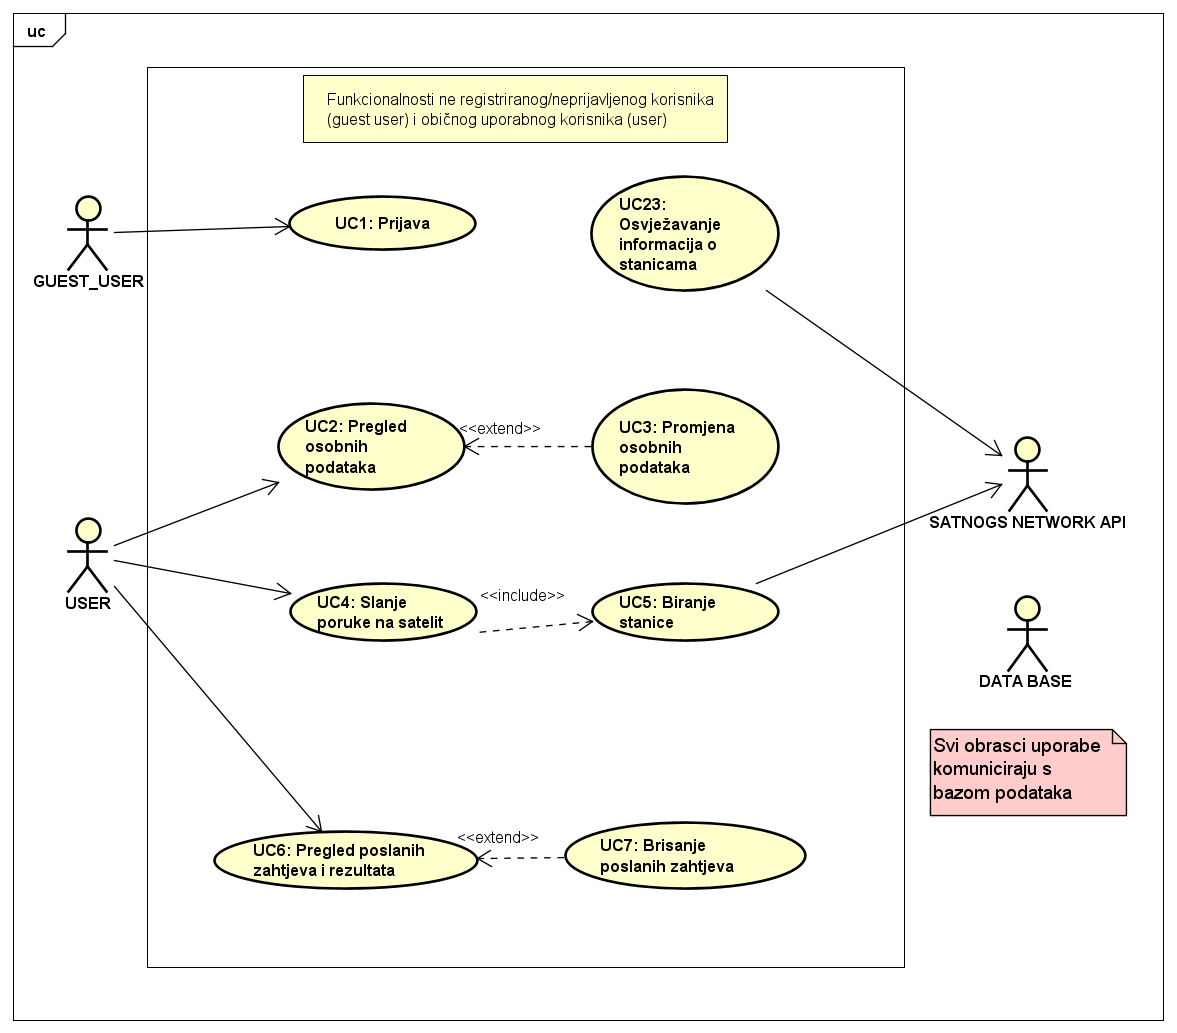
\includegraphics[width=\linewidth]{USECASE1.png}
						\caption{Dijagram obrasca uporabe, funkcionalnost neprijavljenog korisnika i običnog uporabnog korisnika}
						
					\end{figure}
				\begin{figure}[H]
					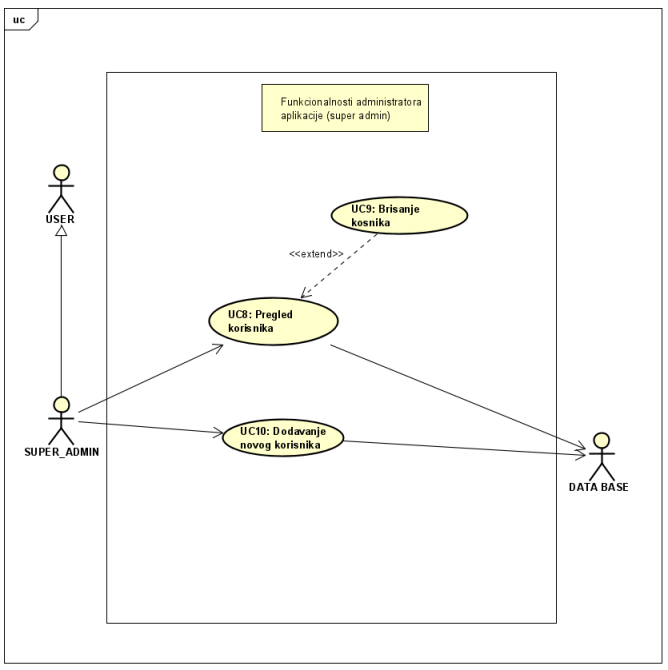
\includegraphics[width=\linewidth]{USECASE2.png}
					\caption{Dijagram obrasca uporabe, funkcionalnost Administratora stranice}
					\label{fig:Dijagrami obrazaca uporabe 8-10}
				\end{figure}
			\begin{figure}[H]
				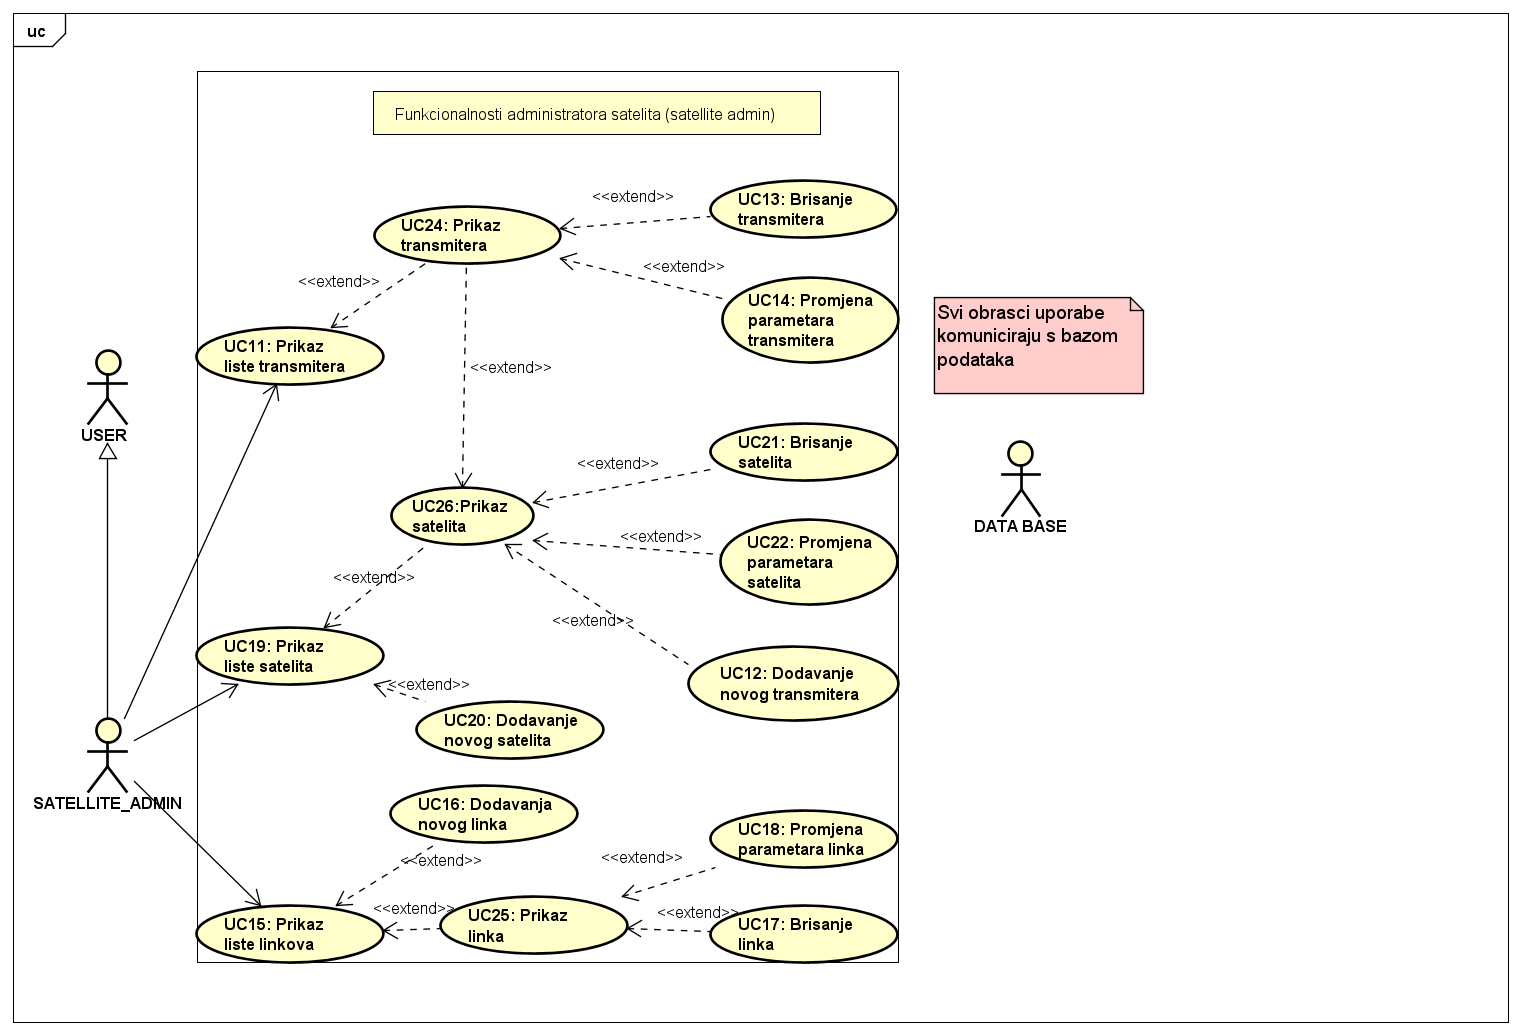
\includegraphics[width=\linewidth]{USECASE3.png}
				\caption{Dijagram obrasca uporabe, funkcionalnost Administratora satelita}
				\label{fig:Dijagrami obrazaca uporabe 11-19}
			\end{figure}
					
				\eject		
				
			\subsection{Sekvencijski dijagrami}
				
\textbf{Obrazac uporabe UC1-Prijava}

{Neregistrirani korisnik upisuje korisničko ime i lozinku. Klikom na gumb "Log in" ti podaci se šalju na validaciju. Ako su uneseni podaci pronađeni u bazi, aplikacija generira token sesije. U suprotnom, šalje se poruka o neispravnoj akreditaciji.}

				\begin{figure}[H]
					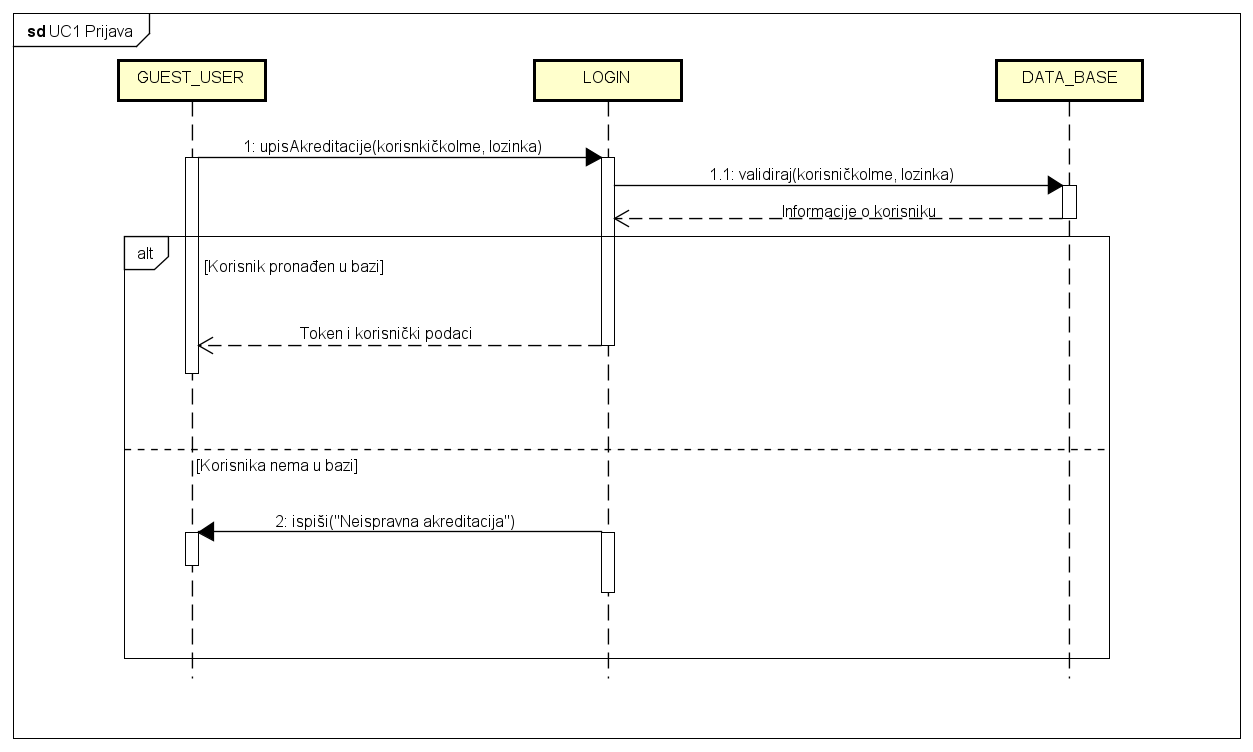
\includegraphics[width=\linewidth]{Sekvencijski1.png}
					\caption{Sekvencijski dijagram prijave korisnika}
					\label{fig:Sekvencijski prijava}
				\end{figure}
			\newpage
			\textbf{Obrazac uporabe UC4-Slanje poruke na satelit}
			
			{Korisnik šalje zahtjev za slanje poruke na satelit. Sustav na taj zahtjev iz baze dohvaća podatke o satelitima te ih šalje natrag korisniku. Korisnik potom bira satelit na koji želi poslati poruku. Aplikacija na taj zahtjev dohvaća listu kompatibilnih linkova za odabrani satelit i šalje ih korisniku. Nakon toga, korisnik odabere jedan link, a zatim se ostvaruje odabir stanice (Vidi \ref{Word:UC5}). Na posljetku, korisnik unosi tekst poruke i pritiskom na gumb "Send" pokreće simulaciju komunikacije sa satelitom. Aplikacija simulira slanje i odgovor koje sprema u bazu, a nakon toga šalje odgovor korisniku. }
		
				\begin{figure}[H]
					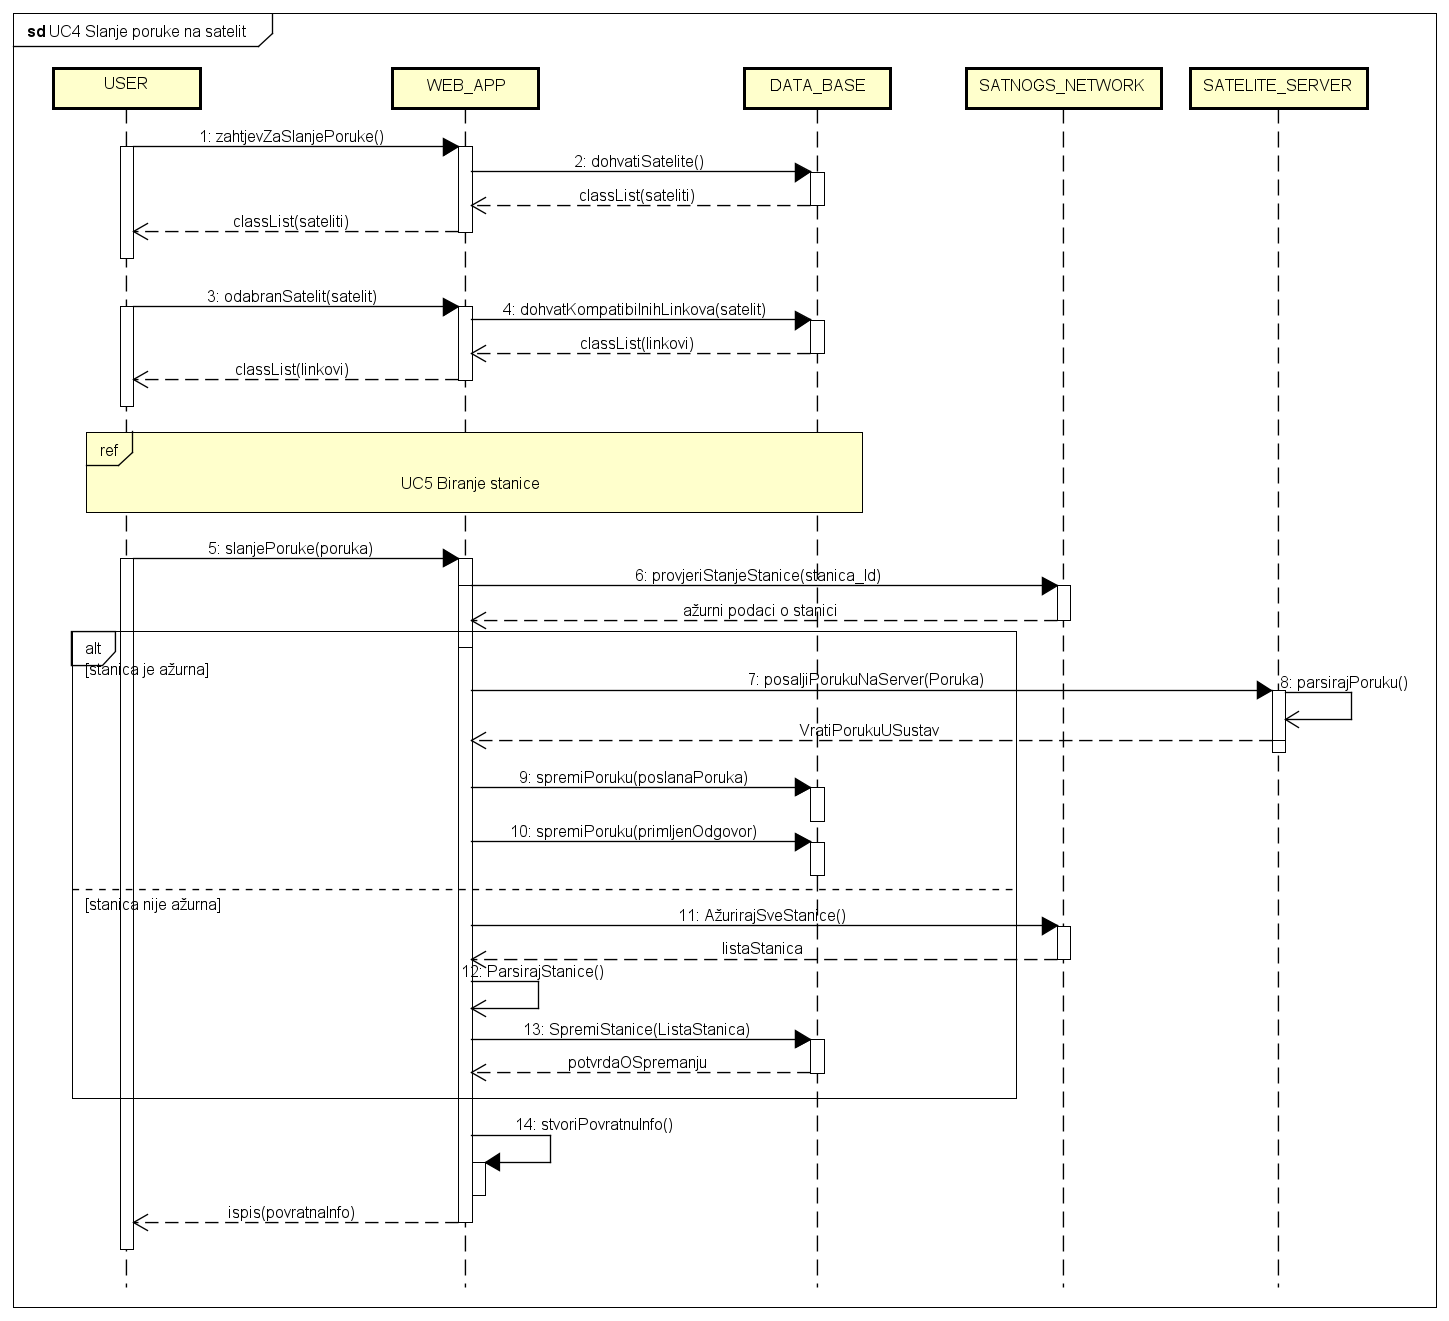
\includegraphics[width=\linewidth]{Sekvencijski2.png}
					\caption{Sekvencijski dijagram slanja poruke}
					\label{fig:Sekvencijski poruka}
				\end{figure}
			\newpage
			\textbf{Obrazac uporabe UC5-Biranje stanice}
			
			{Korisnik odlučuje hoće li odabir stanice prepustiti aplikaciji (automatski) ili samostalno izabrati preko koje stanice će se komunikacija odvijati. Pri odabiru automatske opcije, aplikacija dohvaća iz baze stanice koje su kompatibilne s prethodno odabranim linkom. Odabir optimalne stanice temelji se na atributu broja obzervacija. Iz SatNOGS mreže dohvaćaju se ažurni podaci o odabranoj optimalnoj stanici. Aplikacija uspoređuje podatke o stanici iz baze s dobivenim iz SatNOGS mreže. Ako nije došlo do promjena, korisniku se šalje poruka o pronalasku stanice i on može nastaviti sa slanjem poruke. Ukoliko je došlo do promjena podataka koji utječu na komunikaciju, podaci se u bazi ažuriraju i nastavlja se s traženjem optimalne stanice. U slučaju da stanica više ne postoji u mreži, njen zapis se briše iz baze i ponovno se nastavlja traženje optimalne stanice. \newline
				U drugom slučaju, aplikacija iz baze dohvaća kompatibilne stanice pa šalje upit na SatNOGS mrežu o tim stanicama i po primitku odgovora uspoređuje dobivene podatke s pročitanim podacima iz baze. Ukoliko je došlo do promjena u podacima, ažurira ih u bazi. Zatim, šalje korisniku listu stanice iz koje on treba odabrati željenu stanicu za komunikaciju.}
			
			
				\begin{figure}[H]
					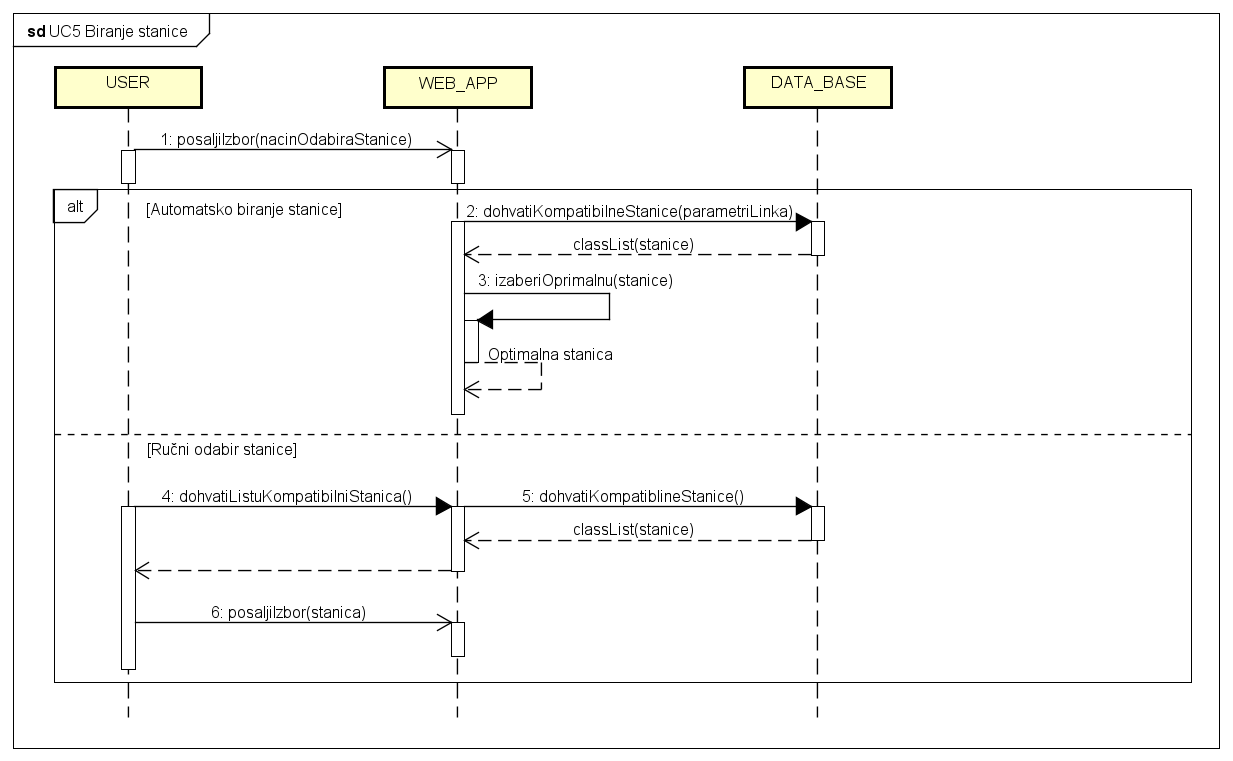
\includegraphics[width=\linewidth]{Sekvencijski3.png}
					\caption{Sekvencijski dijagram biranja stanice}
					\label{fig:Sekvencijski }
				\end{figure}
				
	
		\section{Ostali zahtjevi}
		 
			   \begin{itemize}
                \item Sustav treba biti jednostavan/intuitivan za koristenje, korisnici se moraju znati koristiti sučeljem bez opširnih uputa.
                \item Neispravno korištenje korisničkog sučelja ne smije narušiti funkcionalnost i rad sustava.
                \item Nadogradnja sustava ne smije narušavati postojeće funkcionalnosti sustava.
                \item Lozinke moraju biti kriptirane pri pohrani u bazu.
                \item Sustav treba biti implementiran kao web aplikacija koristeći objektno-\newline orijentirane jezike.
                \item Korisničko sučelje i sustav treba podržavati hrvatske dijakritičke znakove za unos i prikaz tekstualnog sadržaja
                \item Sustavu se treba moći pristupati iz javne mreže pomoću HTTPS
                \item Sustav pri logiranju korisnuku dodjeljuje JWT Token kako bi se garantirao siguran prijenos informacija putem web-a
                \item Sustav omogućava istovremeni rad više korisnika

            \end{itemize}
			 
			 
	
	\chapter{Arhitektura i dizajn sustava}
		\graphicspath{{./slike/}}
\noindent Arhitektura sustava može se podijeliti na tri glavna podsustava, a to su: web preglednik, web poslužitelj i baza podataka.

\begin{itemize}
	
	\item  \textbf{Web preglednik} je program koji služi za pristup web stranicama. Putem web preglednika, korisnik šalje zahtjeve za resursima (npr. HTML kod web stranice) ili šalje podatke (npr. putem neke forme), web preglednik dohvaća te datoteke s web poslužitelja, a potom ih interpretira i prikazuje na ekranu korisnika ili ih pohranjuje na poslužitelju. 
	
	\item \textbf{Web poslužitelj} glavni je dio web aplkacije. To je namjensko računalo ili softver koji šalje i prima podatke od mnogostrukih klijenata. Komunikacija s klijentima (korisnicima i bazom podataka) odvija se preko HTTP protokola. Na korisnikov zahtjev, web preglednik dohvaća resurse i vraća u obliku HTML dokumenta ili obrađuje podatke predane u formi te ih sprema u bazu podataka. 

	\item \textbf{Baza podataka} koristi se za pohranjivanje podataka sustava. Web aplikacija u svom radu vrlo često komunicira s bazom te iz nje dohvaća podate ili ih u nju sprema. 
\end{itemize}
Pri oblikovanju aplikacije koristili smo MVC (Model-View-Controller) obrazac softverske arhitekture.
Po principu MVC-a, aplikaciju dijelimo na tri komponente:	

\begin{itemize}
	
	\item \textbf{Model} je glavna komponenta sustava. Predstavlja strukturu podataka (Java objekti) i njihovu funkcionalnost.
	
	\item \textbf{View} odlučuje kako će se dohvaćeni podaci reprezentirati.
	
	\item \textbf{Controller}  zaprima zahtjeve za resursima (HTTP zahtjevi) od klijenta koje prilagođava i prosljeđuje Modelu ili Viewu. 
	
\end{itemize}
Programski jezik kojeg smo odabrali za izradu backenda naše aplikacije je Java zajedno sa Spring Boot radnim okvirom u razvojnom okruženju Intellij, a u izradi frontenda koristili smo jezike JavaScript i TypeScript te biblioteke React, Redux i Axios uz razvojno okruženje Visual Studio Code. 







	
		

		

				
		\section{Baza podataka}
			
			
		\textit {\normalfont} U ovom projektu koristit ćemo relacijsku bazu u kojoj će gradivne jedinke biti entiteti, definirani imenom i skupom atributa. Zadaća baze je pohrana podataka o satelitima, linkovima, baznim stanicama i korisnicima. Sukladno time entiteti koje ćemo kreirati su:

        \begin{itemize}
            \item User
            \item Satellite
            \item Transmitter
            \item Link
            \item Station
            \item Antenna
            \item Message
        \end{itemize}
		
			\subsection{Opis tablica}
			

				\textbf{User} {\normalfont} Ovaj entitet sadrži podatke o korisniku                aplikacije. Njegovi atributi su:\newline userId (PRIMARY KEY), username, email,         password i roleName.
                    Ovaj entitet u vezi je \emph{One-to-Many} s entitetom Satellite preko atributa userId, u vezi \emph{One-to-Many} s entitetom Link preko atibuta userId i u vezi \emph{One-to-Many} s entitetom Message preko atributa userId.
				
				
				\begin{longtblr}[
					label=none,
					entry=none
					]{
						width = \textwidth,
						colspec={|X[6,l]|X[6, l]|X[20, l]|}, 
						rowhead = 1,
					} %definicija širine tablice, širine stupaca, poravnanje i broja redaka naslova tablice
					\hline \SetCell[c=3]{c}{\textbf{User}}	 \\ \hline[3pt]
					\SetCell{LightGreen}userId & INT	&  Jedinstveni brojčani identifikator, autogeneriran od strane baze  	\\ \hline
				\SetCell{LightBlue} username	& VARCHAR &  Jedinstveno korisničko ime\\ \hline 
					\SetCell{LightBlue} email & VARCHAR &  Jedinstvena email adresa \\ \hline 
					password & VARCHAR	&  Šifrirana lozinka\\ \hline 
                    roleName & VARCHAR & SUPER\_ADMIN (admin aplikacije), SATELLITE\_ADMIN (admin satelita) ili USER (običan korisnik)\\ \hline
				\end{longtblr}

                     \textbf{ Satellite} {\normalfont} Ovaj entitet sadrži podatke o satelitima u Zamljinoj orbiti. Njegovi atributi su: satelliteId (PRIMARY KEY), satName i satelliteStatus.
                    Ovaj entitet u vezi je \emph{Many-to-One} s entitetom User preko atributa userId, u vezi \emph{Many-to-Many} s entitetom Transmitter preko atributa satelliteId i transmId.

                    \begin{longtblr}[
					label=none,
					entry=none
					]{
						width = \textwidth,
						colspec={|X[6,l]|X[6, l]|X[20, l]|}, 
						rowhead = 1,
					} %definicija širine tablice, širine stupaca, poravnanje i broja redaka naslova tablice
					\hline \SetCell[c=3]{c}{\textbf{Satellite}}	 \\ \hline[3pt]
					\SetCell{LightGreen}satelliteId & INT	&  	Jedinstveni brojčani identifikator, autogeneriran od strane baze  	\\ \hline
					\SetCell{LightBlue} satName	& VARCHAR &   Naziv satelita\\ \hline 
					satelliteStatus & VARCHAR &  Active (dostupan/aktivan) ili inactive (nedostupan/neaktivan)\\ \hline  
				\end{longtblr}

                    \textbf{Transmitter} {\normalfont} Ovaj entitet sadrži podatke o transmiterima koji se nalaze na satelitu. Njegovi atributi su: transmId (PRIMARY KEY), transmFreq, transmMode, transmBaud i transmName.
                    Ovaj entitet u vezi je \emph{Many-to-Many} s entitetom Satellite preko atributa satelliteId i transmId i u vezi \emph{Many-to-One} s entitetom Link preko atributa linkId.
				
				
				\begin{longtblr}[
					label=none,
					entry=none
					]{
						width = \textwidth,
						colspec={|X[6,l]|X[6, l]|X[20, l]|}, 
						rowhead = 1,
					} %definicija širine tablice, širine stupaca, poravnanje i broja redaka naslova tablice
					\hline \SetCell[c=3]{c}{\textbf{Transmitter}}	 \\ \hline[3pt]
					\SetCell{LightGreen}transmId & INT	&  Jedinstveni brojčani identifikator, autogeneriran od strane baze  	\\ \hline
				transmFreq & VARCHAR & Frekvencija na kojoj transmiter može komunicirati\\ \hline
                    transmMode & VARCHAR & Radio-frekvencijska modulacija transmitera (oznaka za način kodiranja informacije u u radio-signalu)\\ \hline
					transmBaud & VARCHAR & Broj kodiranih informacija (definiranih modeom transmitera) koje se mogu promijeniti u jedinici vremena\\ \hline
                    \SetCell{LightBlue}transmName & VARCHAR & naziv transmitera\\ \hline
				\end{longtblr}

                    \textbf{ Link} {\normalfont} Ovaj entitet sadrži podatke o linkovima koji predstavljaju vezu između entiteta Satellite i entiteta Station. Njegovi atributi su: linkId (PRIMARY KEY), linkMode, linkBaud i linkFreq.
                    Ovaj entitet u vezi je \emph{Many-to-Many} s entitetom Antenna preko atributa linkId i antennaId, u vezi \emph{Many-to-One} s entitetom User preko atributa userId i u vezi \emph{One-to-Many} s entitetom Transmitter preko atributa linkId.

                    \begin{longtblr}[
					label=none,
					entry=none
					]{
						width = \textwidth,
						colspec={|X[6,l]|X[6, l]|X[20, l]|}, 
						rowhead = 1,
					} %definicija širine tablice, širine stupaca, poravnanje i broja redaka naslova tablice
					\hline \SetCell[c=3]{c}{\textbf{Link}}	 \\ \hline[3pt]
					\SetCell{LightGreen}linkId & INT	&  	Jedinstveni brojčani identifikator, autogeneriran od strane baze  	\\ \hline
					linkMode	& VARCHAR & Radio-frekvencijska modulacija linka (oznaka za način kodiranja informacije u u radio-signalu)\\ \hline 
                    linkBaud	& VARCHAR & Broj kodiranih informacija (definiranih modeom linka) koje se mogu promijeniti u jedinici vremena\\ \hline 
					linkFreq & INT &  Frekvencija na kojoj se uspostavlja komunikacija između satelita i bazne stanice \\ \hline 
									\end{longtblr}

                     \textbf{ Station} {\normalfont} Ovaj entitet sadrži podatke o zemaljskim stanicama (dobivene iz satNOGS Network API-ja) koje komuniciraju sa Zemaljskim satelitima preko linkova. Njegovi atributi su: stationId (PRIMARY KEY), numOfObservations, statName, altitude, longitude, latitude i stationStatus.
                     Ovaj entitet je u vezi \emph{Many-to-Many} s entitetom Antenna preko atributa antennaId i stationId.

                    \begin{longtblr}[
					label=none,
					entry=none
					]{
						width = \textwidth,
						colspec={|X[6,l]|X[6, l]|X[20, l]|}, 
						rowhead = 1,
					} %definicija širine tablice, širine stupaca, poravnanje i broja redaka naslova tablice
					\hline \SetCell[c=3]{c}{\textbf{Station}}	 \\ \hline[3pt]
					\SetCell{LightGreen}stationId & INT	&  	jedinstveni brojčani identifikator	\\ \hline
				
					numOf-
                    Observations & INT & broj uspješno obavljenih slanja i dohvaćanja podataka sa satelita \\ \hline 
				    statName & VARCHAR	&  	Naziv Zemaljste stanice\\ \hline 
                    altitude & INT	&  Nadmorska visina lokacije na kojoj se nalazi stanica\\ \hline 
                    longitude & DECIMAL(3,2)	& Geografska dužina lokacije na kojoj se nalazi stanica\\ \hline 
                    latitude & DECIMAL(3,2)	&  Geografska širina lokacije na kojoj se nalazi stanica\\ \hline
                    stationStatus & VARCHAR & Offline (nije u mreži), testing (u fazi testiranja) ili online (u mreži je)\\ \hline 
				\end{longtblr}

                    \textbf{ Antenna} {\normalfont} Ovaj entitet sadrži podatke o anteni koja se nalazi na stanici (dobivene iz satNOGS Network API-ja). Njegovi atributi su: antennaId (PRIMARY KEY), antennaType, antennaFreqHigh i antennaFreqLow.
                    Ovaj entitet u vezi je \emph{Many-to-Many} s entitetom Station preko atributa antennaId i stationId, u vezi \emph{Many-to-Many} je s entitetom Link preko atributa linkId i antennaId.

                    \begin{longtblr}[
					label=none,
					entry=none
					]{
						width = \textwidth,
						colspec={|X[6,l]|X[6, l]|X[20, l]|}, 
						rowhead = 1,
					} %definicija širine tablice, širine stupaca, poravnanje i broja redaka naslova tablice
					\hline \SetCell[c=3]{c}{\textbf{Antenna}}	 \\ \hline[3pt]
					\SetCell{LightGreen}antennaId & INT	&  	Jedinstveni brojčani identifikator, autogeneriran od strane baze  	\\ \hline
					antennaType	& VARCHAR & Tip antene\\ \hline 
					antennaFreq-
                    High & INT & Gornja granica frekvencije na kojoj antena može komunicirati \\ \hline 
					antennaFreq-
                    Low & INT &  Donja  granica frekvencije na kojoj antena može komunicirati	\\ \hline 
				\end{longtblr}

                    \textbf{ Message} {\normalfont} Ovaj entitet sadrži podatke o porukama koje je korisnik slao na neki od satelita i rezultatima koje je od njega dobio. Njegovi atributi su: messageId (PRIMARY KEY), satelliteId, message i timestampOfMessage.
                    Ovaj entitet u vezi je \emph{Many-to-One} s entitetom User preko atributa userId.

                    \begin{longtblr}[
					label=none,
					entry=none
					]{
						width = \textwidth,
						colspec={|X[6,l]|X[6, l]|X[20, l]|}, 
						rowhead = 1,
					} %definicija širine tablice, širine stupaca, poravnanje i broja redaka naslova tablice
					\hline \SetCell[c=3]{c}{\textbf{Message}}	 \\ \hline[3pt]
					\SetCell{LightGreen}messageId & INT	&  	Jedinstveni brojčani identifikator, autogeneriran od strane baze  	\\ \hline
					satelliteName	& VARCHAR &  Ime satelita koji se koristio u komunikaciji \\ \hline
					stationIName	& VARCHAR &  Ime stanice kroz koju teće komunikacija \\ \hline 
					message & VARCHAR & tekst poruke koja je poslana/primljena \\ \hline 
					timestampOf-
                    Message & TIMESTAMP	&   Vrijeme i datum slanja/primanja poruke	\\ \hline 
				\end{longtblr}
			
			\subsection{Dijagram baze podataka}
				
					\begin{figure}[H]
					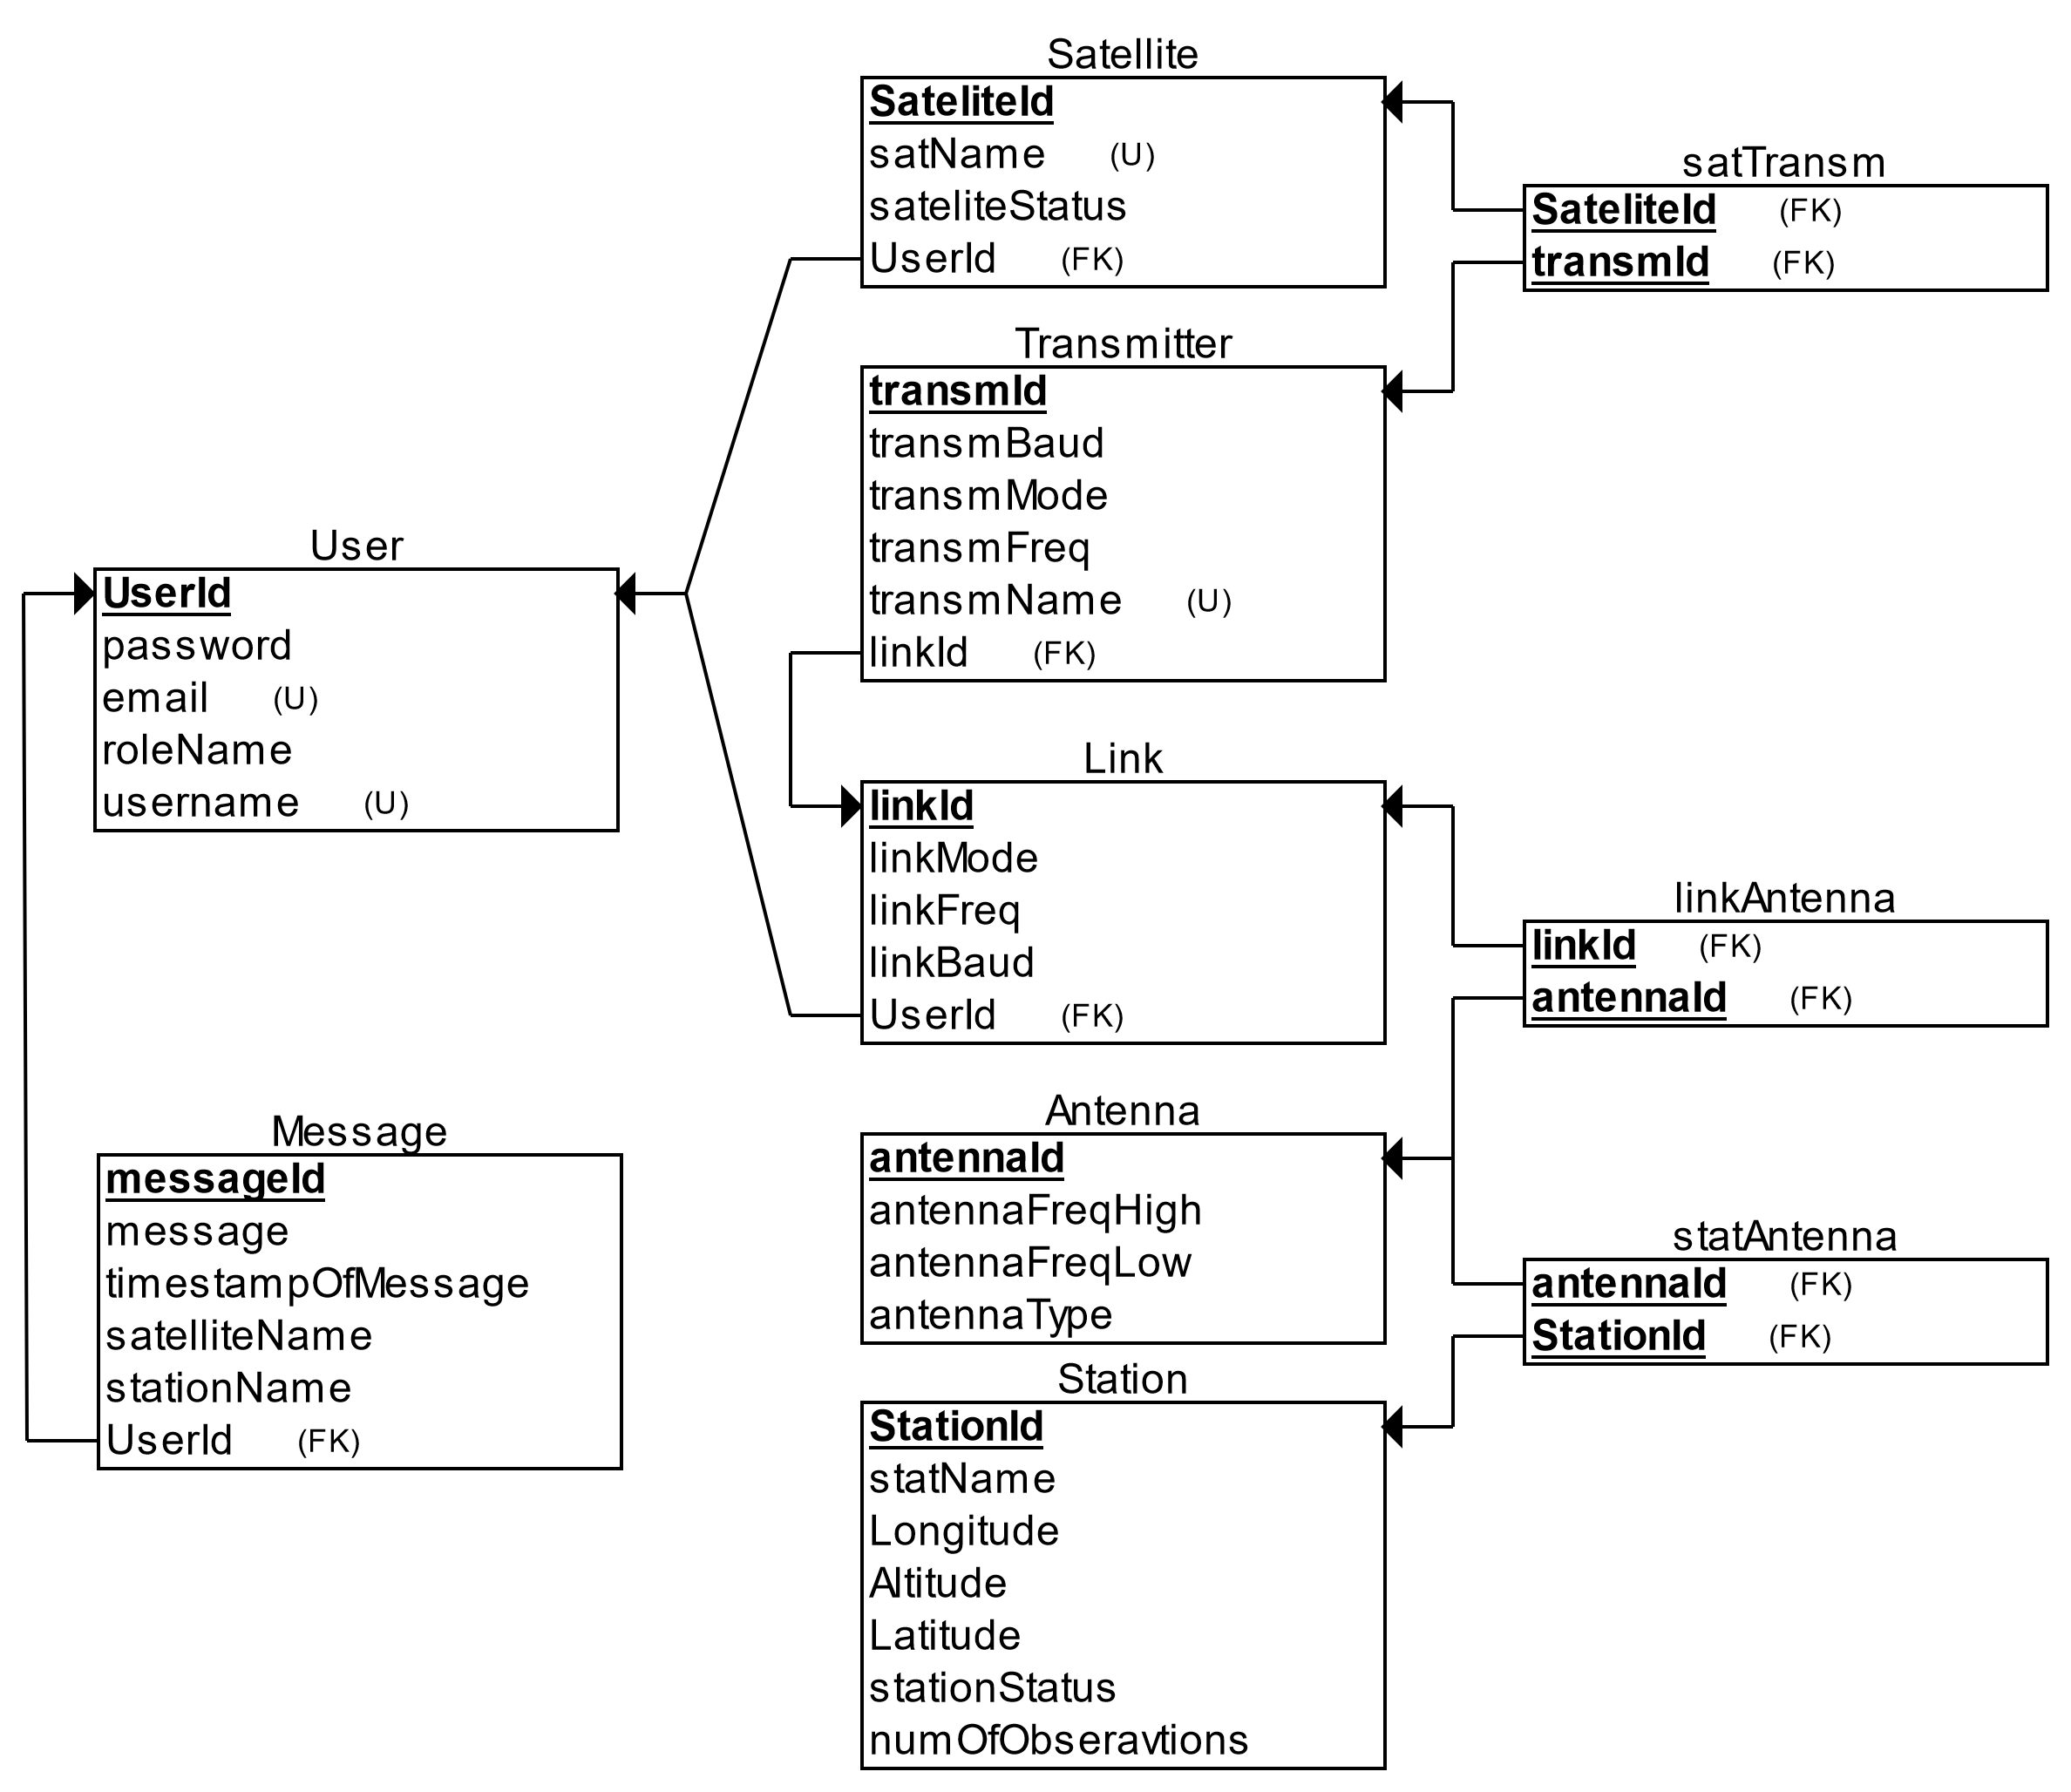
\includegraphics[width=\linewidth]{DB_Diagram.png}
					\caption{Dijagram baze podataka}
					\label{fig:Dijagram baze podataka}
				\end{figure}
			
			\eject
		\section{Dijagram razreda}
		{Na slikama \ref{fig:razredi_controllers} i \ref{fig:razredi_models} prikazani su razredi koji odgovaraju \textit{backend} dijelu MVC arhitekture. Razredi prikazani na slici \ref{fig:razredi_controllers} nasljeđuju Controller razred. Metode implementirane u tim razredima manipuliraju modelima i vraćaju zatražene podatke koji su reprezentirani modelima u listama.}
		
		
		{Model razredi preslikavaju strukturu baze podataka u aplikaciji. Razredi prikazani na \ref{fig:razredi_models} su Java klase koji predstavljaju entitete iz baze podataka. Članske varijable svake klase su atributi odgovarajućeg entiteta iz baze.}
		\begin{figure}[H]
			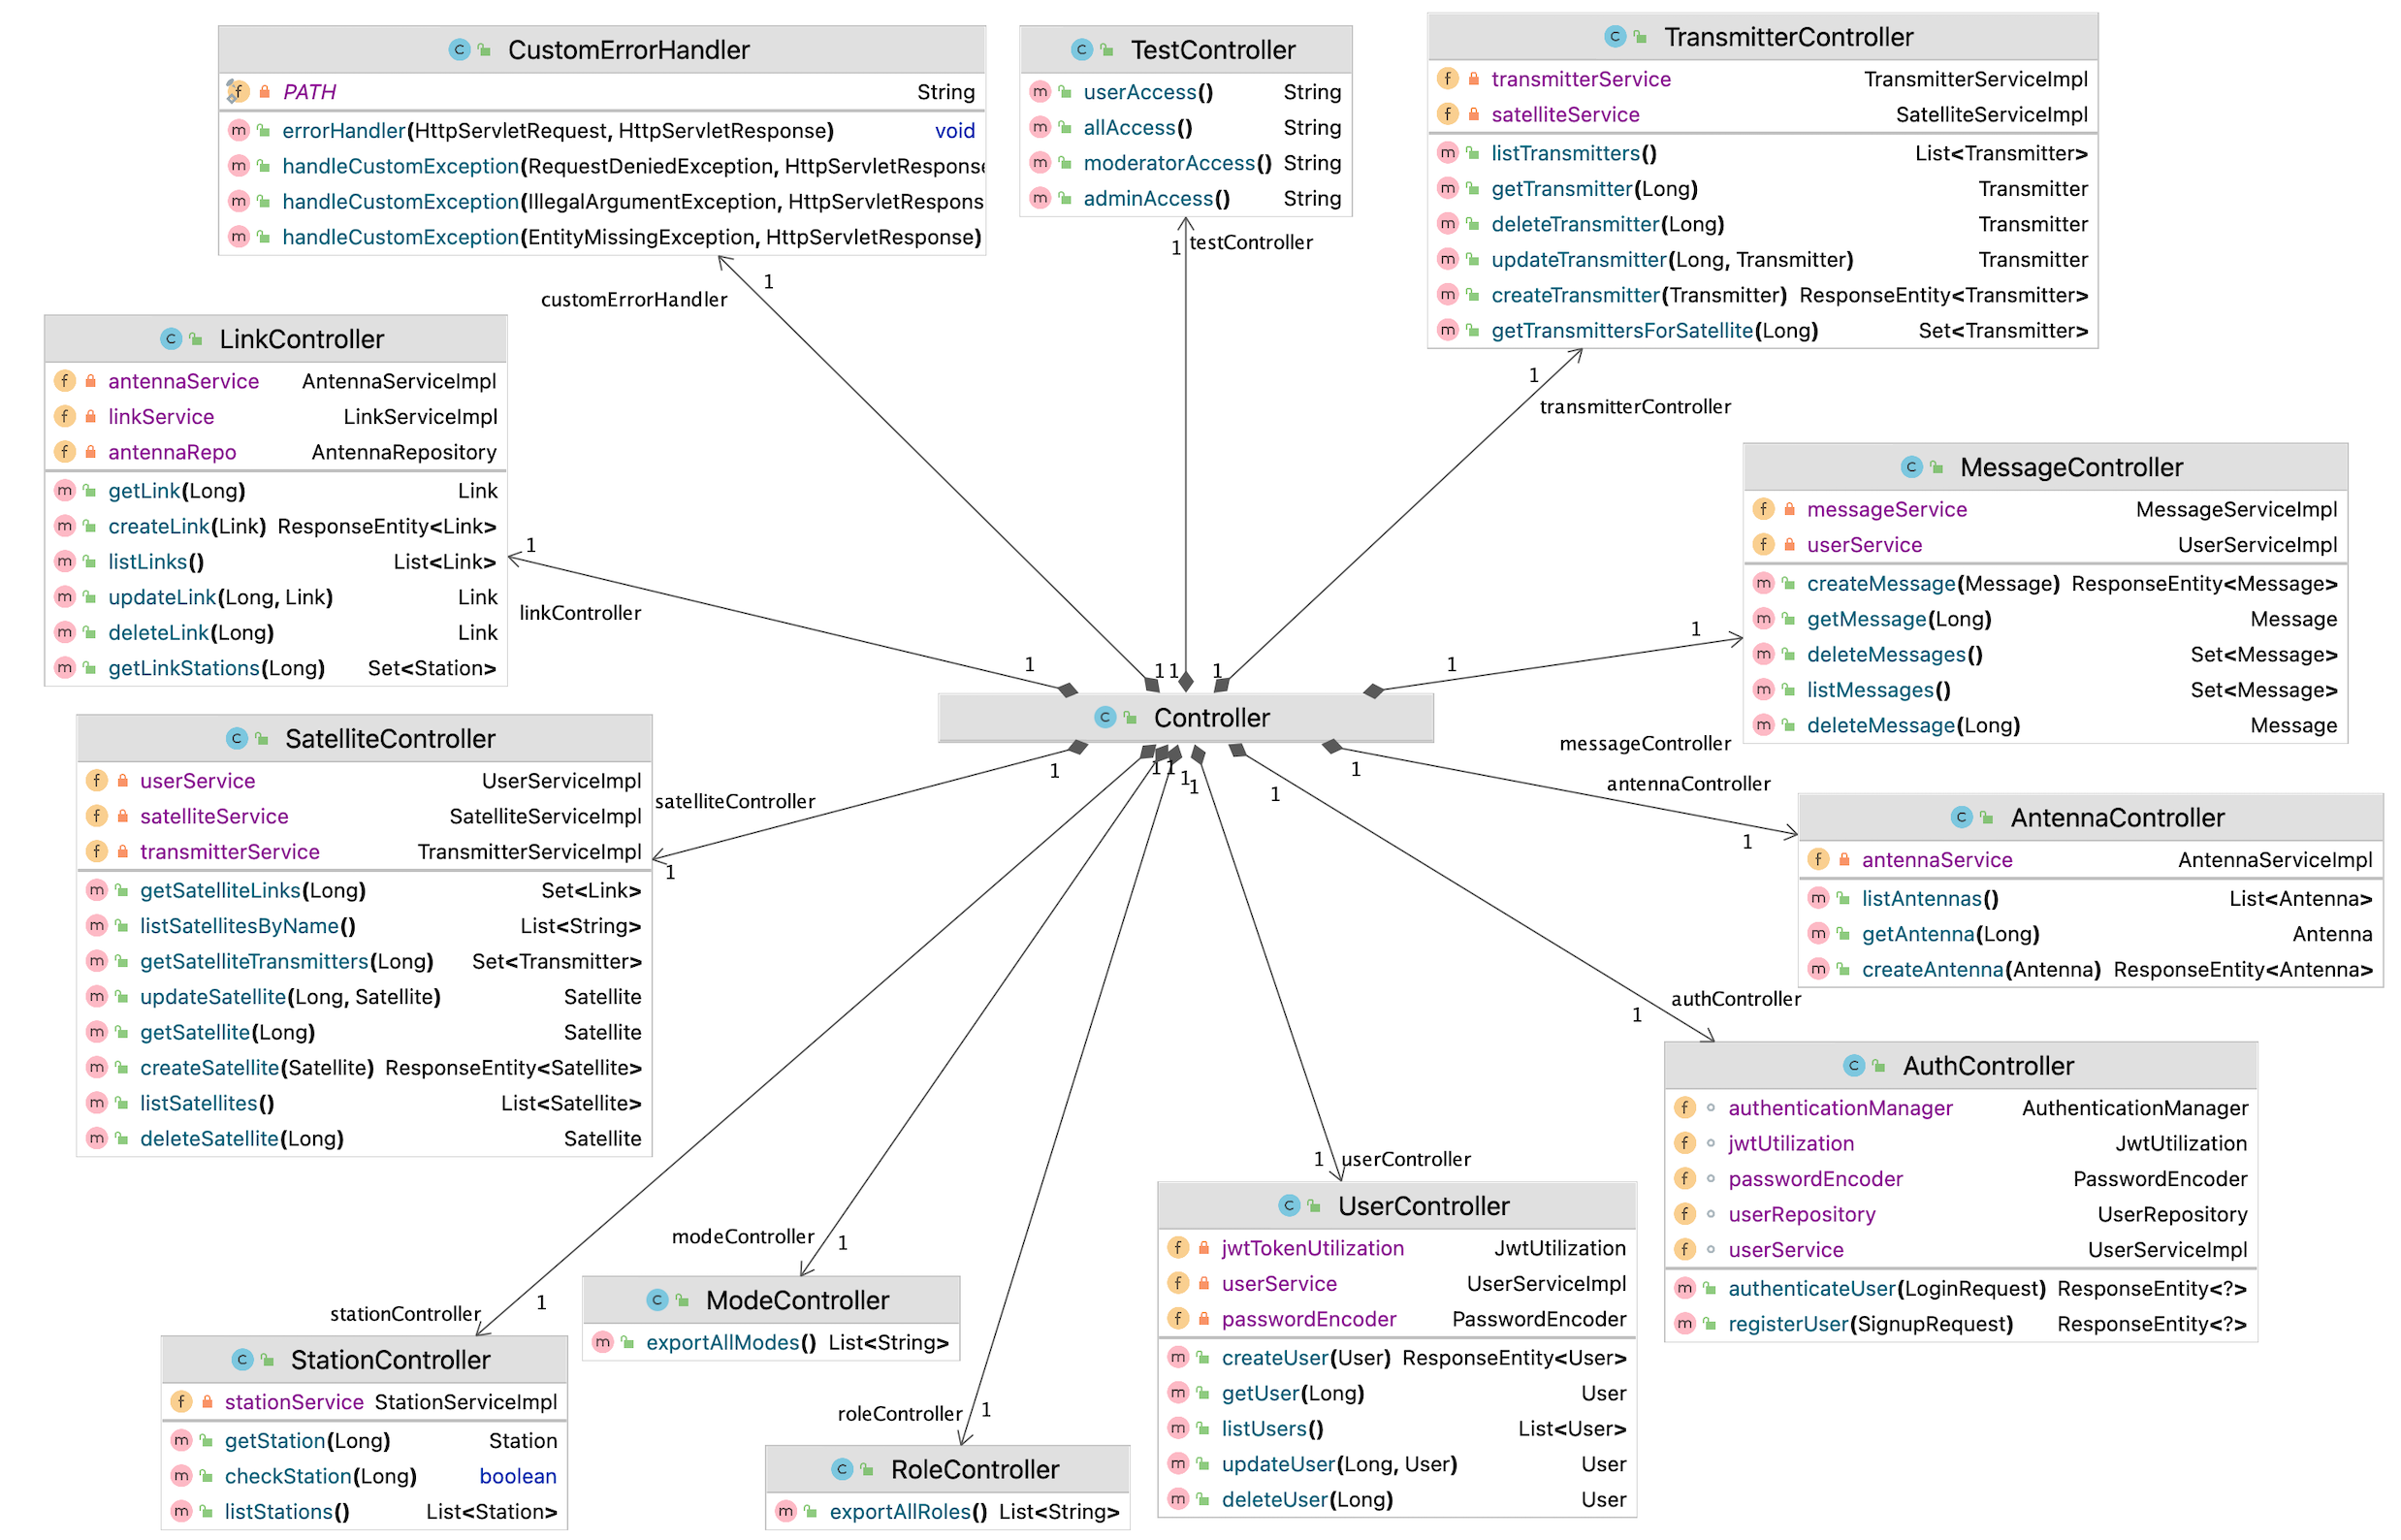
\includegraphics[width=\linewidth]{Diagram_razreda_kontrole.png}
			\caption{Dijagram razreda Controllers}
			\label{fig:razredi_controllers}
		\end{figure}
	
		\begin{figure}[H]
		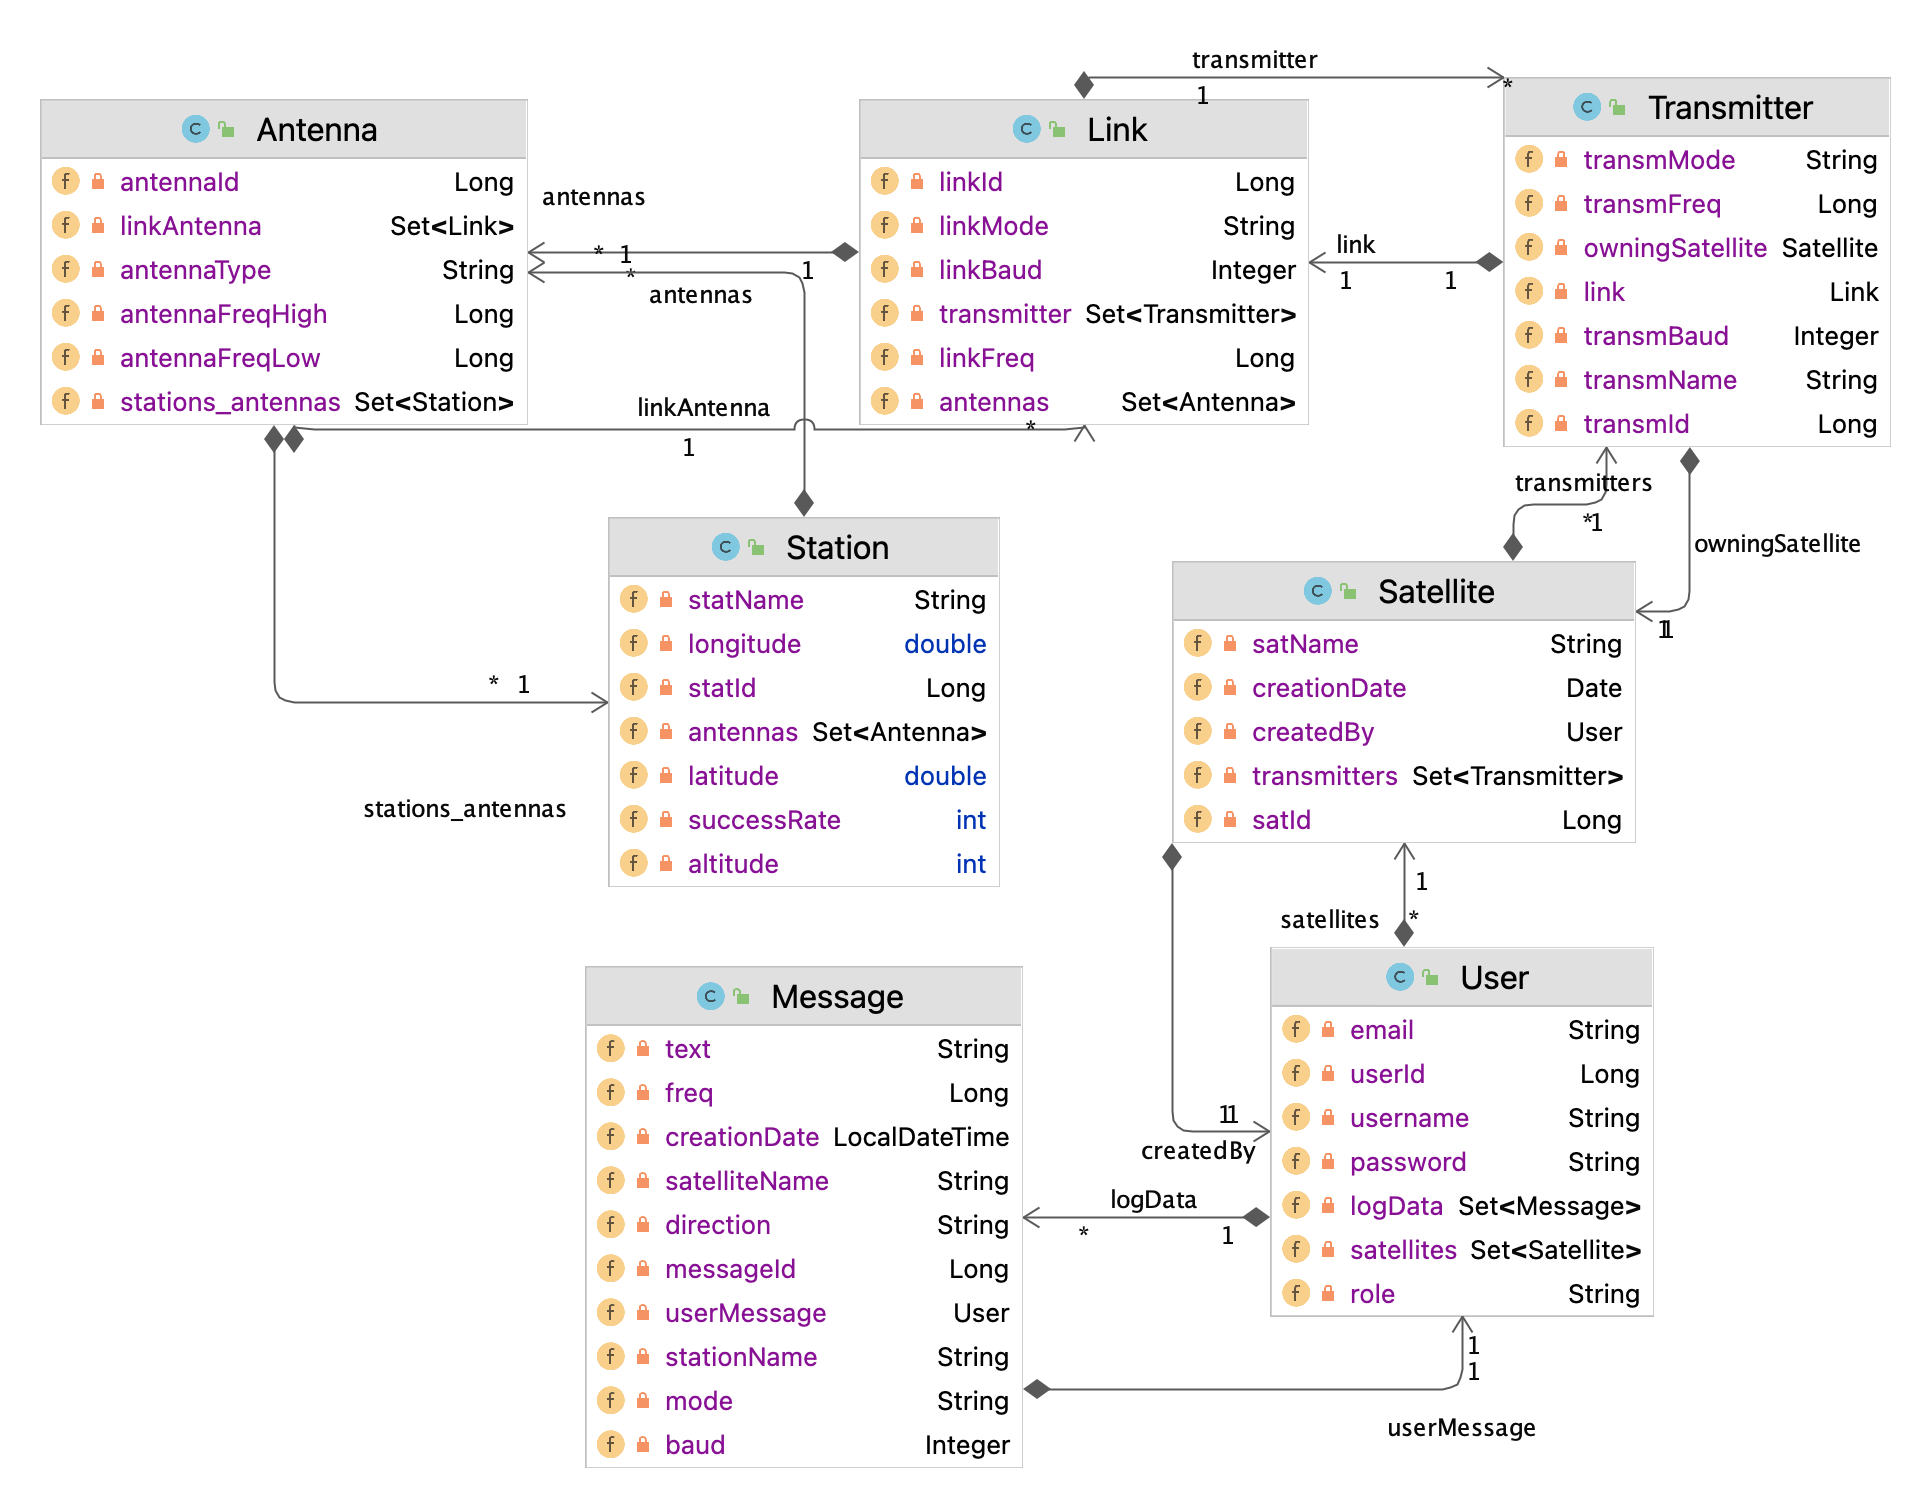
\includegraphics[width=\linewidth]{Diagram_razreda_modela.png}
		\caption{Dijagram razreda Models}
	\label{fig:razredi_models}
\end{figure}


		
		
		
		\eject
		\section{Dijagram stanja}
		
		
		{	Na slici  \ref{fig:dijagramStanja} je prikaz dijagrama stanja koji predstavlja stanja kroz koje korisnik (superadmin, admin satalita ili 
		običan korisnik) prolaze od trenutka prijave, pa sve do trenutka odjave iz web aplikacije. Početno stanje 
		za sve korisnike je prijava. Nakon prijave svim korisnicima je prikazana početna stranica "Home page" gdje se
		nalaze opcije za daljnje korištenje ovisno o ulozi.
		Svim korisnicima je zajedničko slanje poruka na prikazu "SEND MESSAGE" gdje se kroz 4 koraka odvija odabir
		satelita, odabir odgovarajučeg linka, zatim odabira načina slanja poruke te u konačnici unos poruke koja će se 
		poslati i slanje poruke. Osim slanja poruke svima je omogućen pregled povijesti poslanih poruka na prikazu 
		"MESSAGE HISTORY" gdje svaki korisnik ima mogućnost brisanja poruka iz tablice poruka. Također, svima je omogućen
		prikaz vlastitih korisničkih podataka i njihovo uređivanje.
		Superadminu je dodatno omogućena opcija dodavanje novih korisnika opcijom "Add User" te prikaz liste 
		trenutno postojećih korisnika u sustavu.
		Korisnik koji ima ulogu admin satelita je u mogućnosti obavljati CRUD akcija kreiranja (eng. create), 
		pregled postojećih podataka (eng. read), uređivanje (eng. update) i brisanje podataka (eng. delete) nad satelitima, 
		linkovima i trensmitterima.
		Zbog preglednosti na dijagramu nije dodana opcija odjava jer iz bilo kojeg prikaza se korisnik može u 
		gornjem desnom kutu odjaviti sa stranice. Također, korisnik se u bilo kojem trenutku može vratiti na početnu 
		stranicu "Home page"}
		
		

		
		
		\begin{figure}[H]
			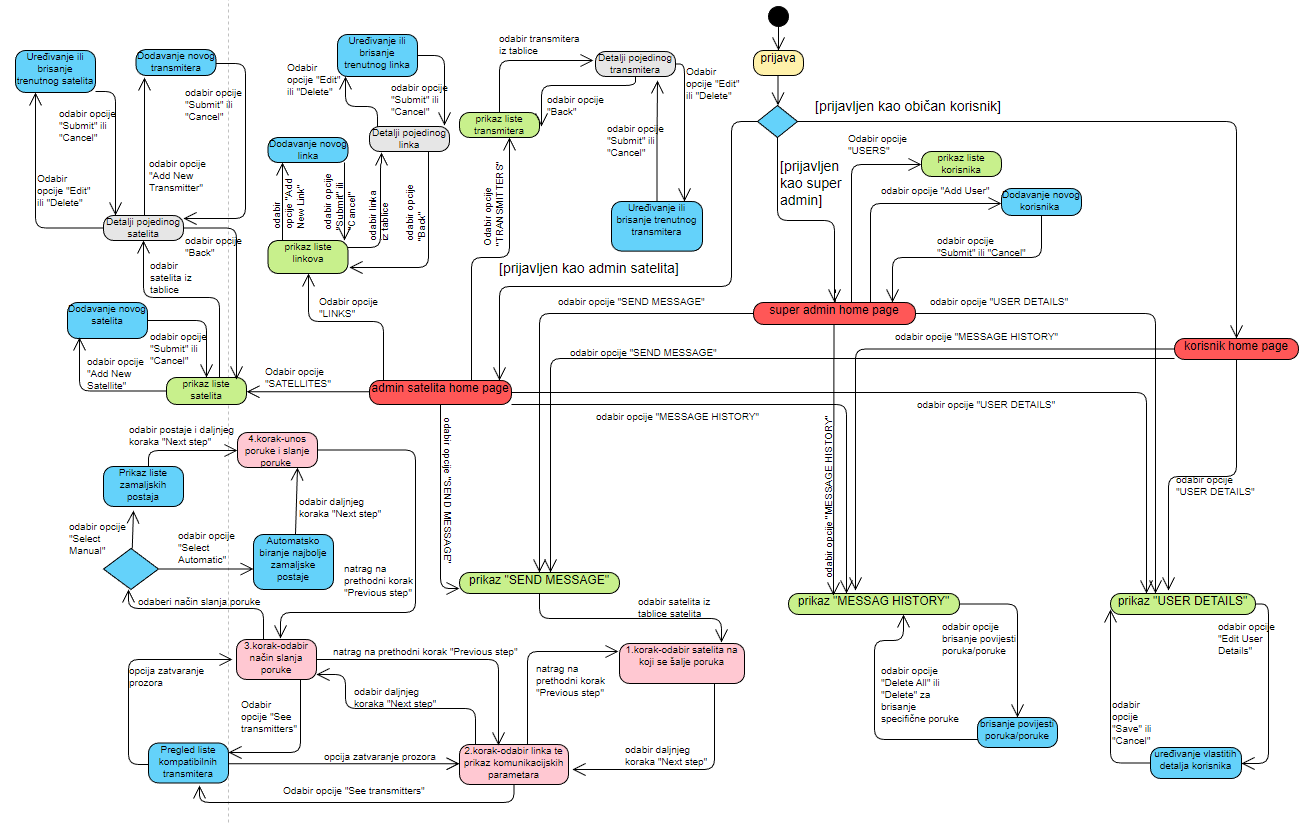
\includegraphics[width=\linewidth]{Diagram_stanja.png}
			\caption{Dijagram stanja}
			\label{fig:dijagramStanja}
		\end{figure}
		
		
		\eject 
		
		\section{Dijagram aktivnosti}
		
				\normalfont{
            Dijagram aktivnosti primjenjujemo za opise modela toka upravljanja ili toka podataka, ali ne i za modeliranje događajima poticanog ponašanja. Pri modeliranju toka upravljanja svaki korak prethodi onom sljedećem u lancu i tim se redom izvršavaju uz naglašenu jednostavnost. Na dijagramu aktivnosti prikazan na slici \ref{fig:dijagramAktivnosti} prikazan je proces slanja poruke na satelit. Prijavljeni korisnik odabire jedan od ponuđenih satelita. Sustav vraća listu kompatibilnih linkova za odabrani satelit. Korisnik zatim odabire link pomoću kojeg želi poslati poruku. Nakon što se odabere link, odabire se i način slanja poruke. Za ručni odabir, sustav vraća stanice koje mogu provesti slanje poruke na satelit uz odabrani link, korisnik zatim odabire željenu stanicu i nastavlja na sljedeći korak. Kod automatskog slanja poruke, stanicu odabire sustav prema najvećem broju obzervacija i korisnik nastavlja na sljedeći korak. Sljedeći korak je ispunjavanje forme za slanje poruke gdje korisnik upisuje željenu poruku i šalje zahtjev za slanje poruke. Kada sustav zaprimi slanje poruke, poruka se prosljeđuje na satelit server gdje se simulira odgovor satelita. Odgovor satelita i poslana poruka se spremaju u bazu podataka te se korisniku prikaže poslana poruka i primljeni odgovor. \newline}
		
		
		\begin{figure}[H]
			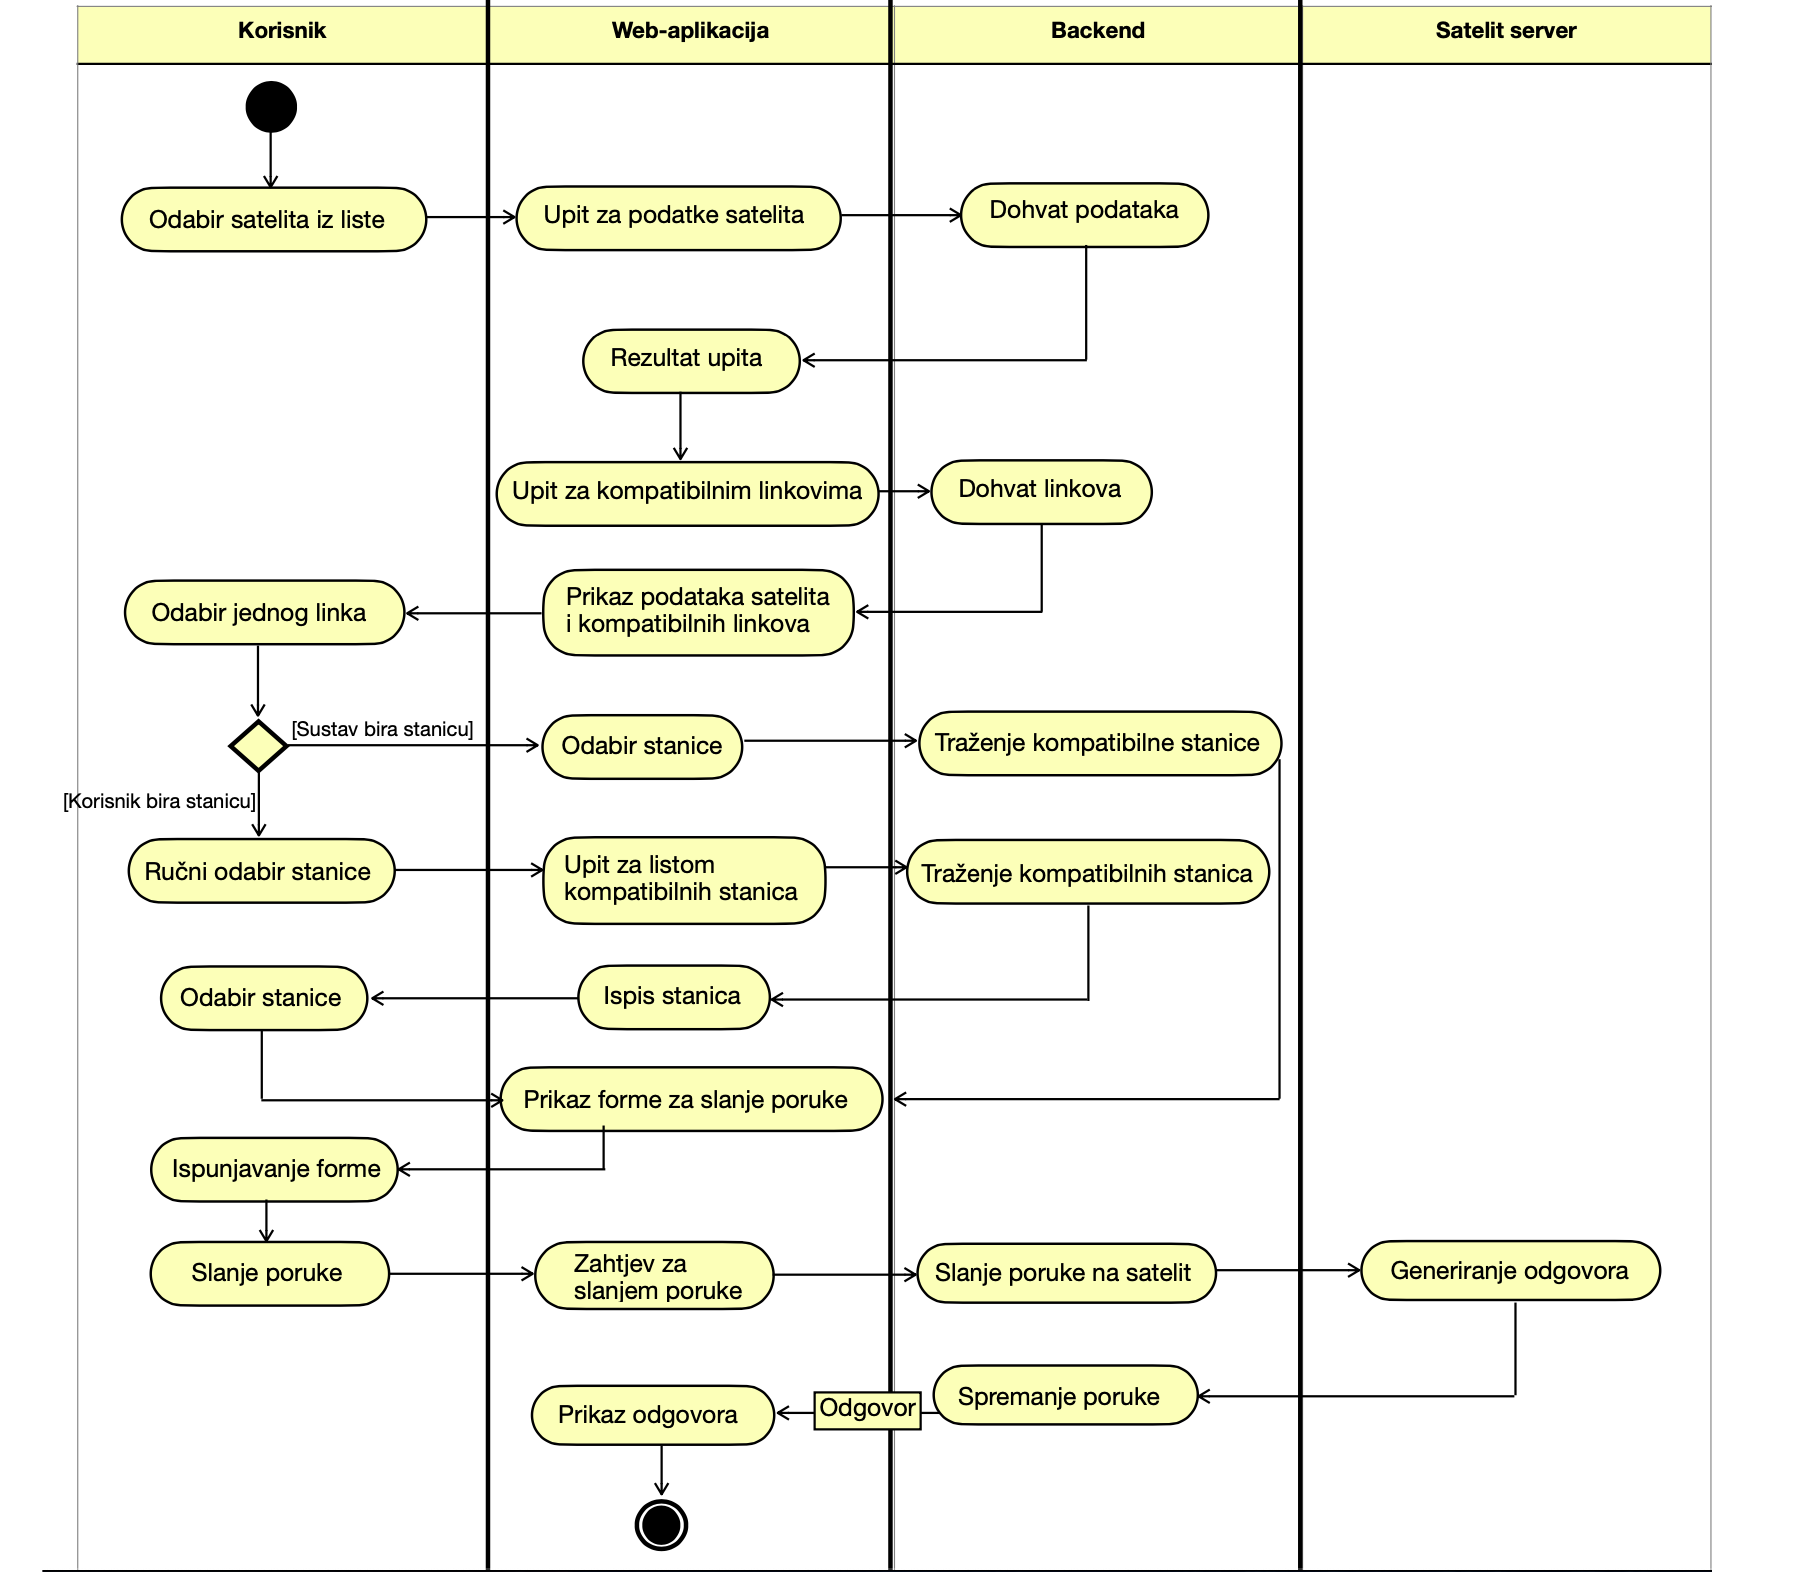
\includegraphics[width=\linewidth]{Activity_diagram.png}
			\caption{Dijagram aktivnosti}
			\label{fig:dijagramAktivnosti}
		\end{figure}
		
		\eject
		\section{Dijagram komponenti}
		
            \normalfont{
            Dijagram komponenti prikazani na slikama \ref{fig:dijagramKomponenti1} i \ref{fig:dijagramKomponenti2} opisuju međuovisnost i organizaciju i odnose u internoj strukturi. Sustavu se pristupa preko internet preglednika preko sučelja za dohvat HTML, CSS i JS datoteka koje služe za prikaz i funkcionalnost grafičkog sučelja. Router je komponenta kojom se upravlja prikaz internet stranice prema ulozi korisnika. Sučelju za primanje JSON podataka pristupa se preko REST API komponenti. Pomoću Axios biblioteke dobivene podatke s \textit{backenda} prenosimo na korisnikov preglednik. Na \textit{backendu} nam je potrebna komponenta Controllers koja služi da modele koje pretvaramo u DTO (\textit{Data transfer object}) pošaljemo na \textit{frontend} i da prenesemo odgovore sa satelita. Paket JpaRepository koristimo za pisanje i čitanje podataka iz vanjske baze podataka. Klase StationChecker i ScheduledTask koriste vansjku aplikaciju SatNOGS za najsvježije podatke potrebne za rad naše aplikacije. \newline}

		\begin{figure}[H]
			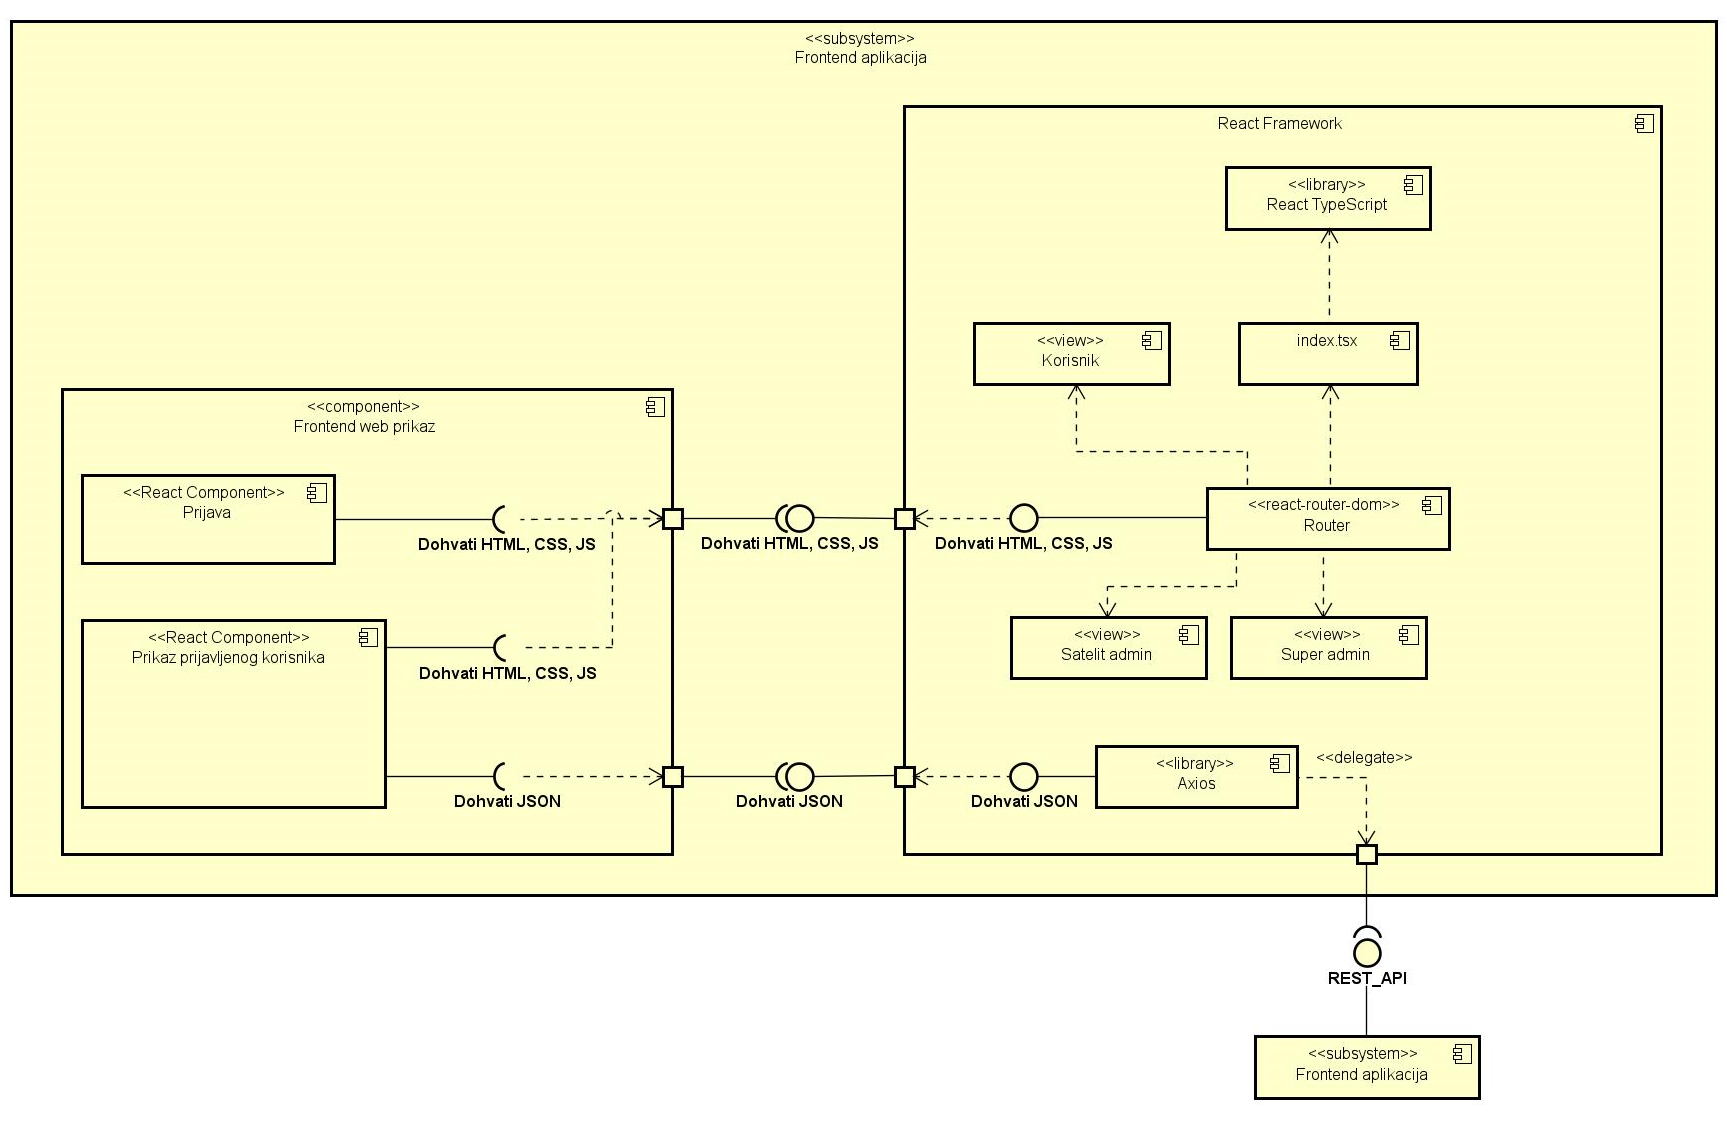
\includegraphics[width=\linewidth]{Component_diagram1.png}
			\caption{Dijagram komponenti frontend dijela aplikacije}
			\label{fig:dijagramKomponenti1}
		\end{figure}
		\begin{figure}[H]
			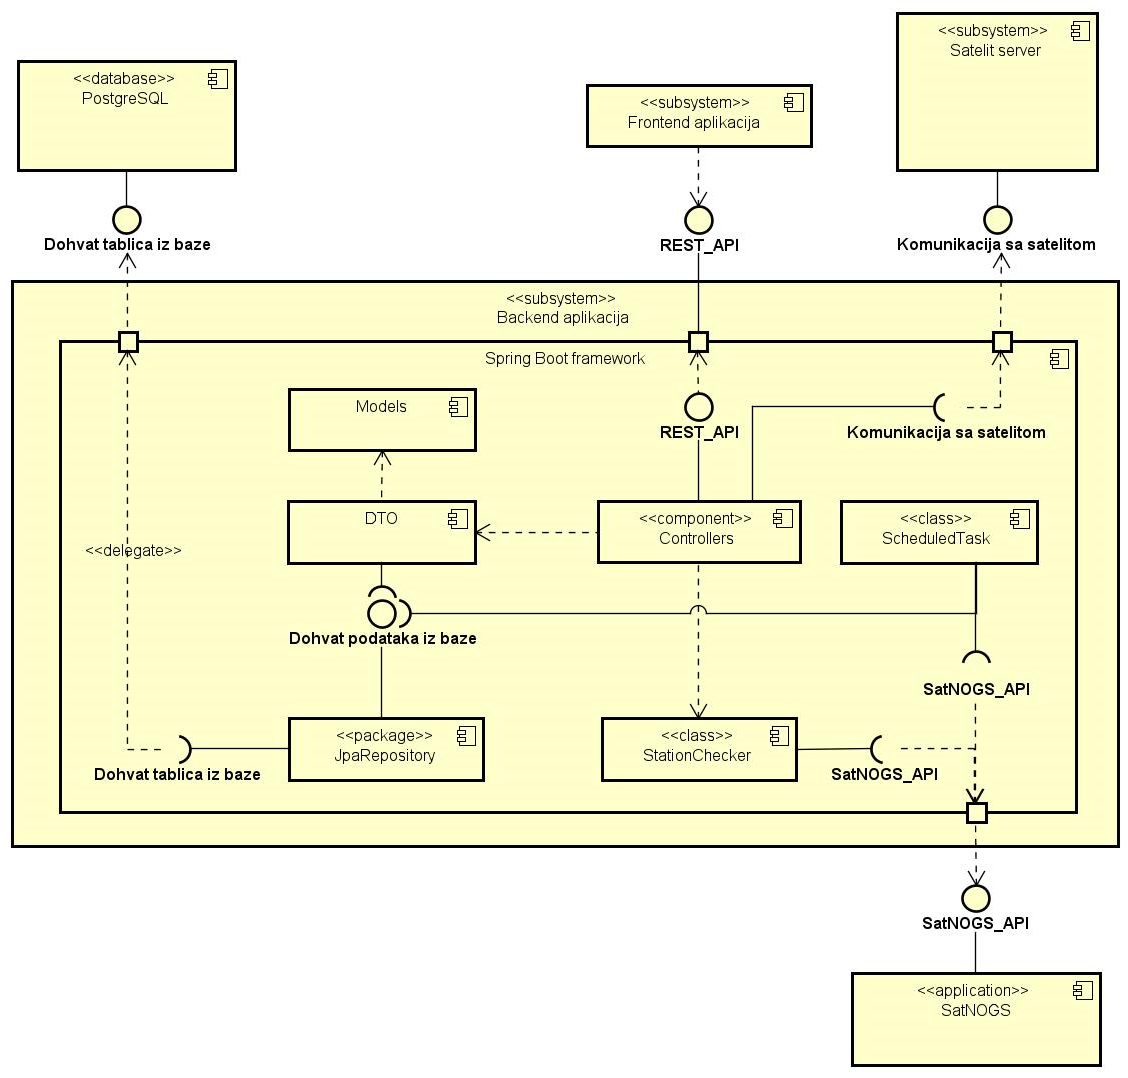
\includegraphics[width=\linewidth]{Component_diagram2.png}
			\caption{Dijagram komponenti backend dijela aplikacije}
			\label{fig:dijagramKomponenti2}
		\end{figure}
	\chapter{Implementacija i korisničko sučelje}
		
		
		\section{Korištene tehnologije i alati}
			{
				Komunikacija u timu je ostvarena korištenjem aplikacija Discord\footnote{\url{https://discord.com/}} i GoogleMeet\footnote{\url{https://meet.google.com/}}.
				Komunikacija s asistentom grupe je ostvarena korištenjem aplikacije MicrosoftOutlook\footnote{\url{https://outlook.live.com/owa/}}.
				Za izradu sekvencijskih UML dijagrama i UML dijagrama obrazaca uporabe korišten je alat Astah UML\footnote{\url{https://astah.net/products/astah-uml/}}. Za izradu UML dijagrama razreda korišten je alat IntelliJ\footnote{\url{https://www.jetbrains.com/idea/}}. Za izradu dijagrama razmještaja korišten je alat VisualParadigmOnline\footnote{\url{https://online.visual-paradigm.com/}}, a za izradu dijagrama aktivnosti korišten je program Pages razvijen od strane Apple Inc.\footnote{\url{https://www.apple.com/pages/}}.
				Za izradu modela baze podataka korišten je alat ERDPlus\footnote{\url{https://erdplus.com/}}.
				Za upravljanje izvornim kodom korišten je alat Git\footnote{\url{https://git-scm.com/}}. Udaljeni repozitorij projekta nalazi se na platformi Gitlab\footnote{\url{https://gitlab.com/}} koja je korištena i za upravljanje zadacima na projektu.
				Kao razvojno okruženje na backendu je korišten IntelliJ, a na frontendu je korišten Visual Studio Code\footnote{\url{https://code.visualstudio.com/}}. Tehnologije korištene za razvoj backenda su radni okvir Spring Boot\footnote{\url{https://spring.io/projects/spring-boot}} i programski jezik Java\footnote{\url{https://www.java.com/en/}}. Tehologije korištene za razvoj frontenda su biblioteka React\footnote{\url{https://reactjs.org/}} i programski jezik JavaScript\footnote{\url{https://www.javascript.com/}}.
				\eject
				Za automatizirano testiranje cjelokupne aplikacije korišten je alat Selenium IDE\footnote{\url{https://www.selenium.dev/selenium-ide/}} te programski jezik Java. 
				Za automatizirano testiranje komponenti korišten je alat JUnit\footnote{\url{https://junit.org/junit5/}} te programski jezik Java.
				Za ručno testiranje korišten je alat ReqBin\footnote{\url{https://reqbin.com/}} te programski jezik Java.
				Za puštanje aplikacije u pogon korištena je platforma MicrosoftAzure\footnote{\url{https://azure.microsoft.com/en-us}}.
		    }
			
			\eject 
		
	
		\section{Ispitivanje programskog rješenja}
			
			\subsection{Ispitivanje komponenti}
			\normalfont{Ispitivanje komponenti ostvareno je pomoću Spring Boot i JUnit 5 alata za ispitivanje. \newline Na slikama \ref{fig:TestCompatibleStationLinkSatellite1} i \ref{fig:TestCompatibleStationLinkSatellite2} prikazani su isječci koda iz testa koji provjerava ispravnost spajanja i dohvaćanja kompatibilne trojke (satelit, link i stanica). Slika \ref{fig:TestCompatibleStationLinkSatellite1} prikazuje dva slučaja: 1. kada satelit, onosno njegovi transmiteri, nisu kompatibilni s linkovima koji se nalaze u bazi. Očekivani rezultat ovog slučaja je prazan set kompatibilnih likova. Te 2. kada postoji link koji je kompatibilan s transmiterom uz očekivani rezultat da set kompatibilnih likova sarži točno jedan link koji je jednak linku kojeg stvaramo u ovom testu. Slika \ref{fig:TestCompatibleStationLinkSatellite2} također prikazuje dva slučaja: 1. kada za određeni link ne postoje kompatibilne stanice, odnosno niti jedna antena neke stanice nije kompatibilna sa zadanim linkom. Očekivani rezultat u ovom slučaju je prazan set kompatibilnih stanica. Te 2. kada postoji stanica s kojom je zadani link kompatibilan. Očekivani rezultat ovog testa je da će set kompatibilnih stanica za zadani link sadržavati jednu stanicu koja je jednaka stanici koju na početnu testa stvaramo.}

            \begin{figure}[H]
					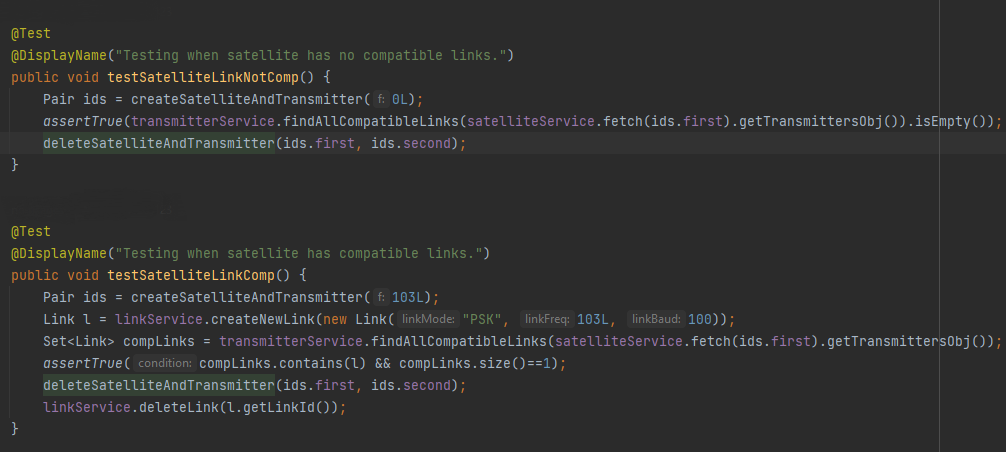
\includegraphics[width=\linewidth]{TestCompatibleStationLinkSatellite1.png}
					\caption{Testiranje spajanja i dohvaćanja kompatibilnih satelita i linkova}
					\label{fig:TestCompatibleStationLinkSatellite1}
				\end{figure}
            \begin{figure}[H]
					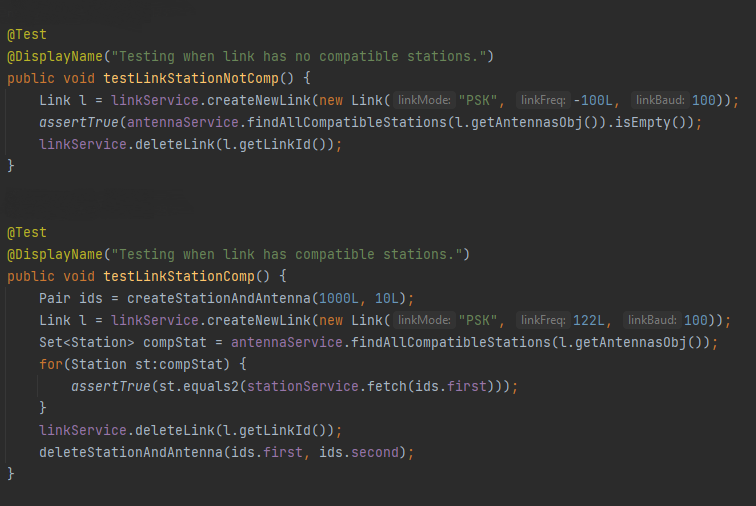
\includegraphics[width=\linewidth]{TestCompatibleStationLinkSatellite2.png}
					\caption{Testiranje spajanja i dohvaćanja kompatibilnih stanica i linkova}
					\label{fig:TestCompatibleStationLinkSatellite2}
				\end{figure}
			
			\normalfont{Na slici \ref{fig:TestStationChecker} prikazano je testiranje funkcionalnosti ispitivanja jednakosti stanica koje su spremljene u bazi u odnosu na stanice koje dohvaćamo sa SatNOGS API-ja. Za prvi test pretpostavka je da stanica s id-jem 6 postoji i u bazi satcom aplikacije i u bazi SatNOGS-a pa je sukladno tome očekivani rezultat istina, tj. stanice su jednake. Pretpostavka za drugi test je da smo u satnogs bazi promijenili barem jedan podatak stanice s id-jem 9 pa je zbog toga očekivai rezultat laž, odnosno da stanice nisu jednake. Pretpostavka za treći test je da smo u satnogs bazi promijenili barem jedan podatak neke antene koja pripada stanici s id-jem 12, tako da možemo očekivati da će rezultat ponovno biti laž, tj. stanice nisu jednake.}

            \begin{figure}[H]
					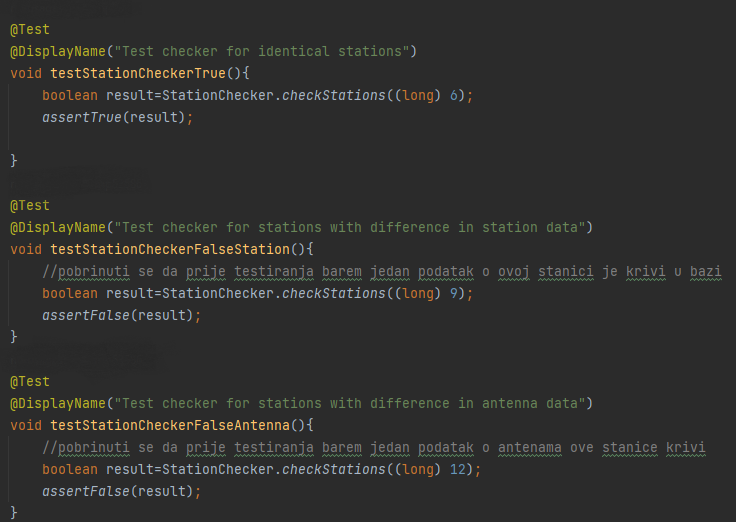
\includegraphics[width=\linewidth]{TestStationChecker.png}
					\caption{Testiranje ispitivanja jednakosti stanica u bazi i na SatNOGS API-ju}
					\label{fig:TestStationChecker}
				\end{figure}
				
			\normalfont{Na slici \ref{fig:TestMessageSaveToDB} prikazano je testiranje spremanja poruke u bazu. Prvi test pokriva slučaj spremanja kada su svi atributi modela Message ispravno postavljeni i očekivani rezultat nakon spremanja je da se u bazi nalazi poruka koja je jednaka onoj koju smo željeli spremiti. Drugi test prikazuje da se u slučaju pokušaja spremanja poruke koja nema sve atribute zadane, konkretno u ovom testnom primjeru atribut satelliteName je null, baca iznimka IllegalArgumentException.}

            \begin{figure}[H]
					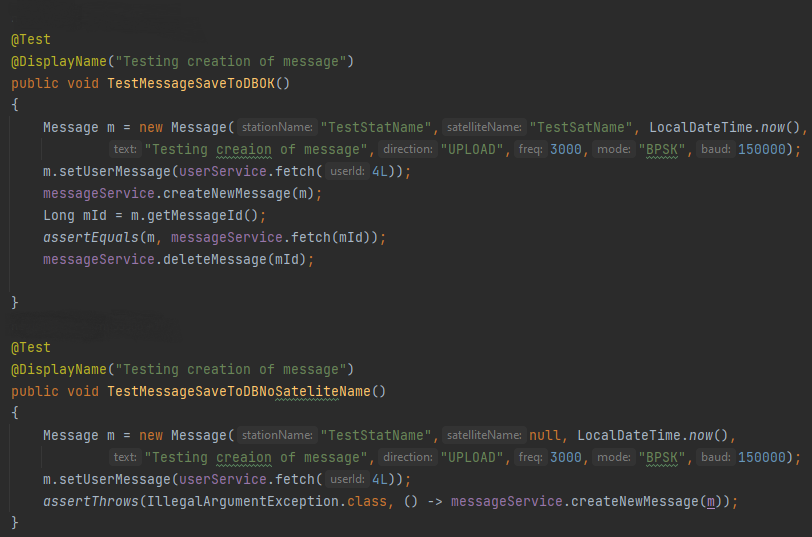
\includegraphics[width=\linewidth]{TestMessageSaveToDB.png}
					\caption{Testiranje spremanja poruka u bazu. }
					\label{fig:TestMessageSaveToDB}
				\end{figure}
				
			\normalfont{Na slikama \ref{fig:TestCommunicationWithSatellite1} i \ref{fig:TestCommunicationWithSatellite2} prikazano je testiranje komunikacije sa serverom kojem šaljemo poruke, tj. koji "glumi" satelit. Test na slici \ref{fig:TestCommunicationWithSatellite1} prikazuje da ako nedostaje neki od argumenata u poruci koju šaljemo, server će vratiti null kao odgovor. Test na slici \ref{fig:TestCommunicationWithSatellite2} prikazuje da ako pošaljemo ispravnu poruku, server će vratiti odgovor koji nije null.}

            \begin{figure}[H]
					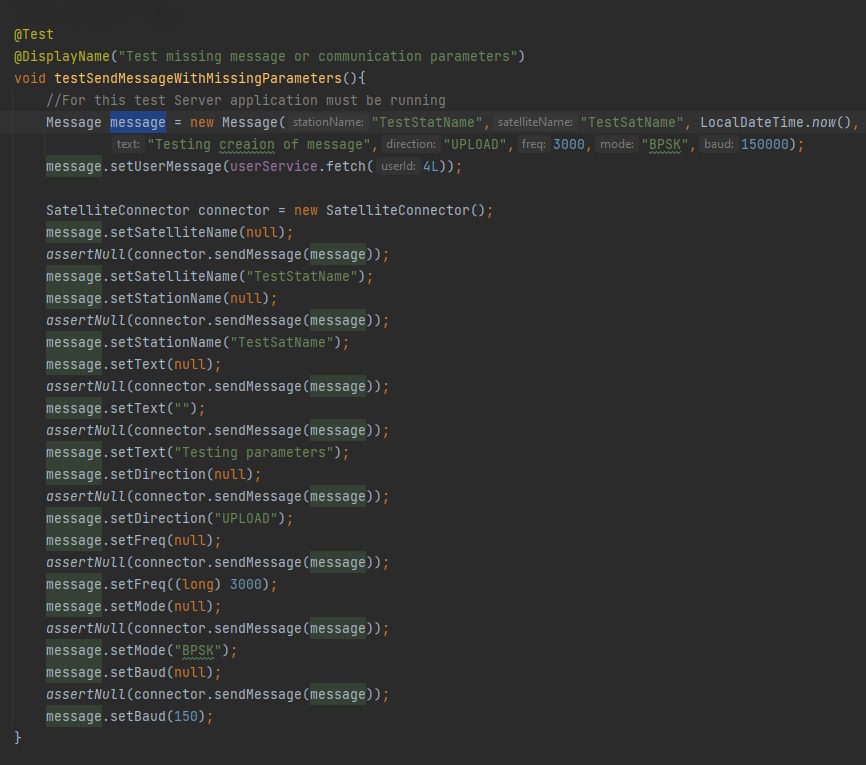
\includegraphics[width=\linewidth]{TestCommunicationWithSatellite1.png}
					\caption{Testiranje neispravne komunikacije sa serverom koji "glumi" satelit.}
					\label{fig:TestCommunicationWithSatellite1}
				\end{figure}
				
			 \begin{figure}[H]
					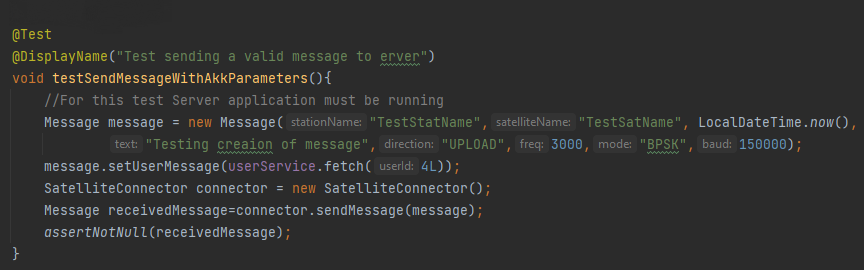
\includegraphics[width=\linewidth]{TestCommunicationWithSatellite2.png}
					\caption{Testiranje ispravne komunikacije sa serverom koji "glumi" satelit.}
					\label{fig:TestCommunicationWithSatellite2}
				\end{figure}
				
			
			
			\subsection{Ispitivanje sustava}
			
            Ispitivanje sustava provedeno je pomoću dodatka za preglednik Selenium IDE. U nastavku su opisani provedeni ispitni slučajevi. \\
            Na slikama \ref{fig:Params1} i \ref{fig:Result1} prikazan je prvi ispitni slučaj u kojem je ispitan pokušaj prijave registriranog korisnika čiji podaci postoje u bazi podataka. Očekivani izlaz je uspješno provedena prijava u sustav i preusmjeravanje na početnu stranicu korisnika. \\

                \begin{figure}[H]
                \centering
				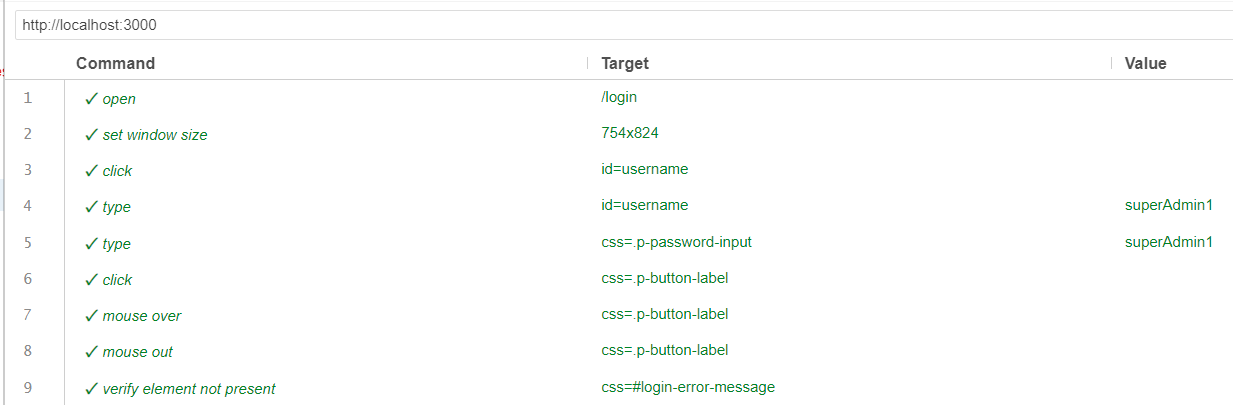
\includegraphics[width=\linewidth]{slike/loginSuccessParams.png}
				\caption{Parametri prvog ispitnog slučaja }
				\label{fig:Params1}
			\end{figure}
   
                 \begin{figure}[H]
                 \centering
				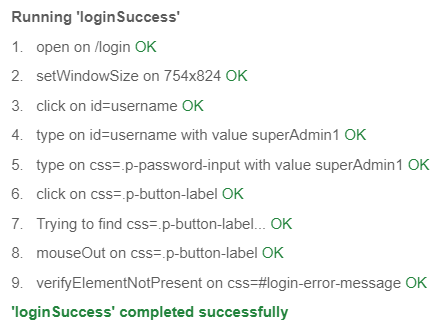
\includegraphics[width=0.5\linewidth]{slike/loginSuccess.png}
				\caption{Rezultat prvog ispitnog slučaja}
				\label{fig:Result1}
			\end{figure}

			\eject
            Slike \ref{fig:Params2} i \ref{fig:Result2} prikazuju drugi ispitni slučaj u kojem je ispitan pokušaj prijave korisnika koji ne postoji u bazi podataka. Očekivani izlaz je neuspješna prijava korisnika u sustav te prikaz poruke pogreške.

                \begin{figure}[H]
                \centering
				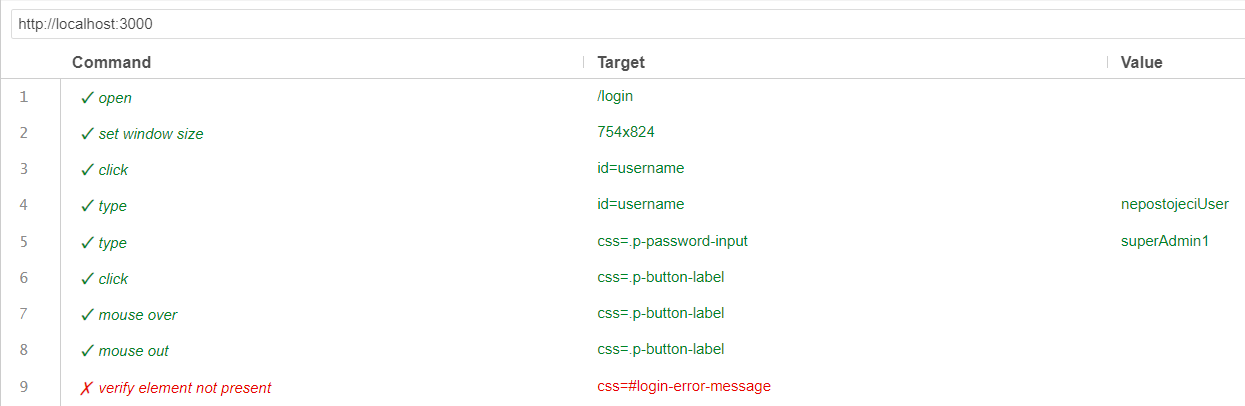
\includegraphics[width=\linewidth]{slike/loginFailParams.png}
				\caption{Parametri drugog ispitnog slučaja }
				\label{fig:Params2}
			\end{figure}
   
                 \begin{figure}[H]
                 \centering
				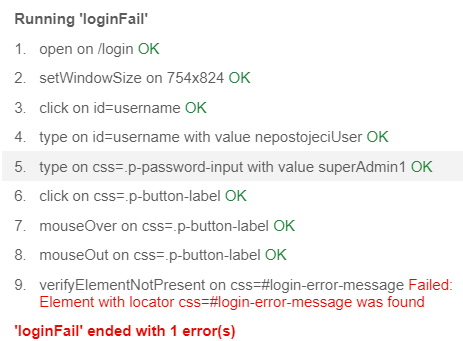
\includegraphics[width=0.5\linewidth]{slike/loginFail.png}
				\caption{Rezultat drugog ispitnog slučaja}
				\label{fig:Result2}
			\end{figure}
			\eject

            Na slikama \ref{fig:Params3} i \ref{fig:Result3} vidimo treći ispitni slučaj koji ispituje registraciju novog korisnika sa valjanim podacima u ispravnom formatu. Očekivani izlaz je uspješna registracija te preusmjeravanje na stranicu Users na kojoj se nalazi lista svih korisnika.

                \begin{figure}[H]
                \centering
				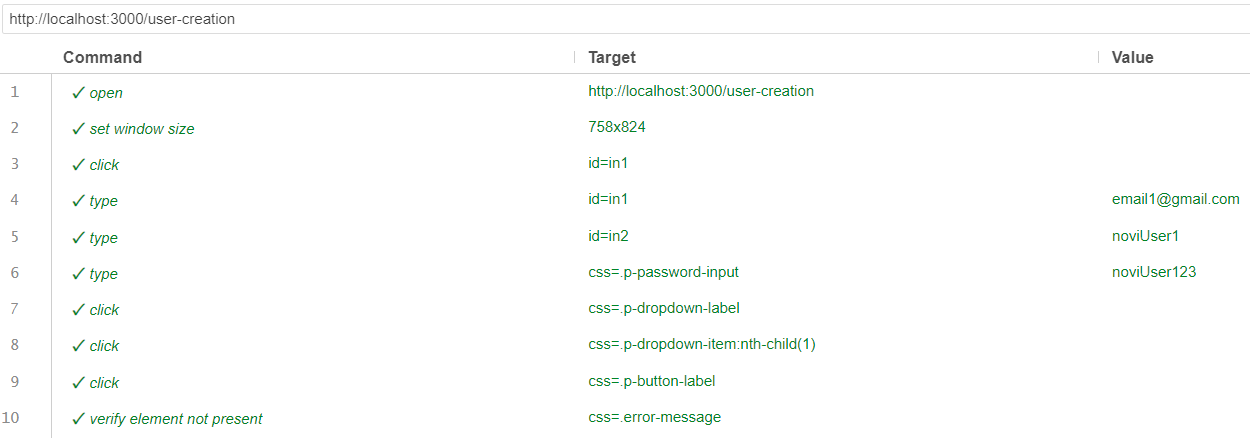
\includegraphics[width=\linewidth]{slike/registerSuccessParams.png}
				\caption{Parametri trećeg ispitnog slučaja }
				\label{fig:Params3}
			\end{figure}
   
                 \begin{figure}[H]
                 \centering
				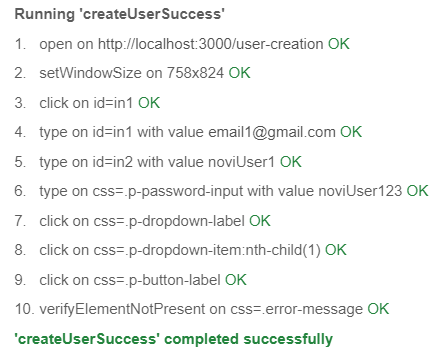
\includegraphics[width=0.5\linewidth]{slike/registerSuccess.png}
				\caption{Rezultat trećeg ispitnog slučaja}
				\label{fig:Result3}
			\end{figure}
			\newpage

            Konačno, Na slikama \ref{fig:Params4} i \ref{fig:Result4} prikazan je četvrti ispitni slučaj u kojem ispitujemo pokušaj registracije korisnika sa neispravnim podacima, odnosno sa e-mail adresom u krivom formatu. Očekivani izlaz je neuspješna registracija te prikaz poruke pogreške.

                \begin{figure}[H]
                \centering
				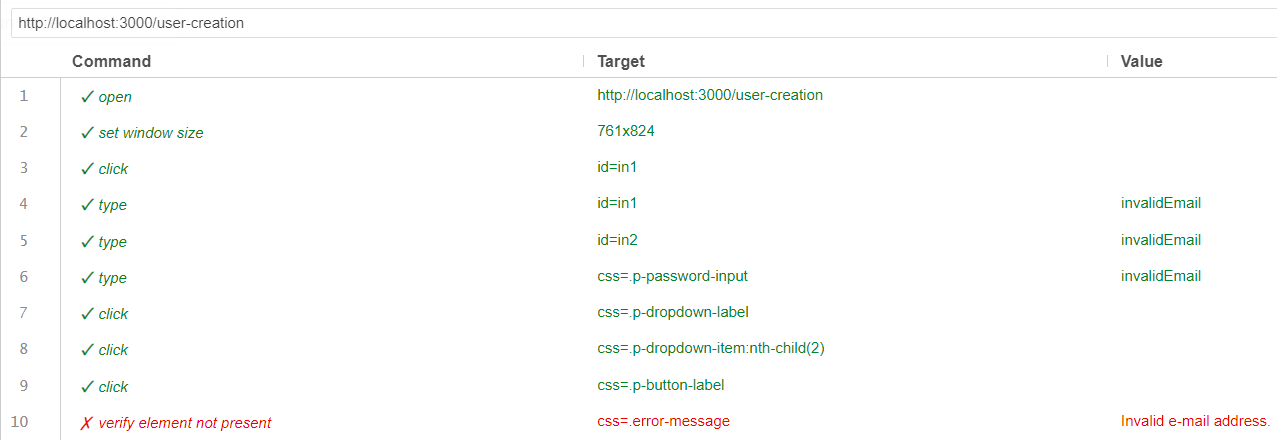
\includegraphics[width=\linewidth]{slike/registerFailParams.png}
				\caption{Parametri četvrtog ispitnog slučaja }
				\label{fig:Params4}
			\end{figure}
   
                 \begin{figure}[H]
                 \centering
				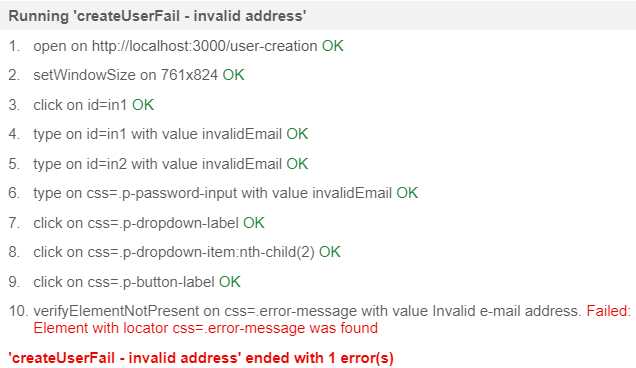
\includegraphics[width=0.5\linewidth]{slike/registerFail.png}
				\caption{Rezultat četvrtog ispitnog slučaja}
				\label{fig:Result4}
			\end{figure}
			
			\eject 
			
		\section{Dijagram razmještaja}
			
			
			
			 Na slici \ref{fig:Dijagram_razmjestaja} prikazan je dijagram razmještaja. Sustav je baziran na arhitekturi "klijent-poslužitelj". Korisnici pristupaju aplikaciji korištenjem web preglednika. Na platformi MicrosoftAzure se nalaze poslužitelji za frontend, backend, bazu podataka te server koji implementira funkcionalnosti satelita. Komunikacija između korisnika i poslužitelja za frontend, te poslužitelja za frontend i poslužitelja za backend, ostvaruje se korištenjem protokola HTTP. Komunikacija između poslužitelja za beckend i servera koji implementira funkcionalnosti satelita odvija se protokolom TCP.
			
			 \begin{figure}[H]
				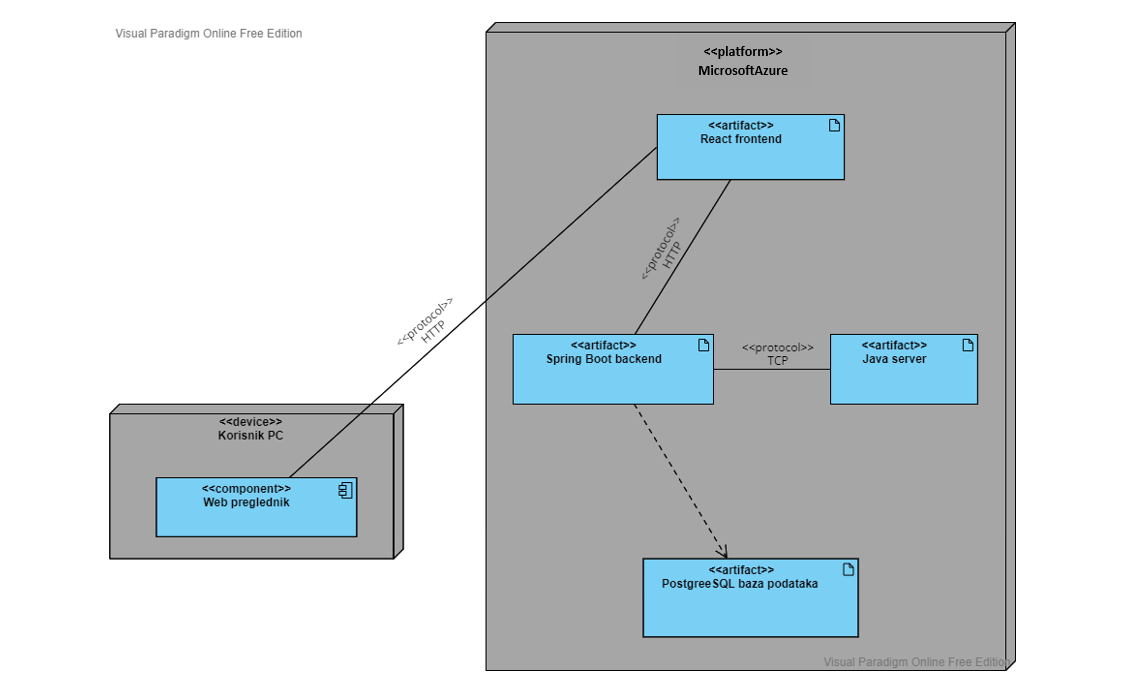
\includegraphics[width=\linewidth]{razmjestaj.png}
				\caption{Dijagram razmještaja}
				\label{fig:Dijagram_razmjestaja}
			\end{figure}
		\newpage
		

			\eject 
		
		\section{Upute za puštanje u pogon}

    Za deploy cjelokupne aplikacije korišten je cloud servis Microsoft Azure čime je omogućeno da aplikacija bude javno dostupna. Na virtualnoj mašini (distribucija Linuxa - Ubuntu 20.04.5), prije samog puštanja aplikacije u pogon, nužno je instalirati potrebnu programsku podršku. Budući da je deployment rađen na virtualnoj mašini u oblaku, sav potrebni softver instaliran je preko komandne linije. U sljedećim odlomcima bit će opisan kompletan postupak postavljanja okruženja za puštanje aplikacije u pogon.
    \newline
    \newline
    \textbf{Konfiguracija backenda}
    
    Za potrebe naše aplikacije nužno je instalirati odgovarajuću Java verziju. U našem slučaju dovoljna je Java 11. Nadalje, potrebno je preuzeti Postgres bazu podataka. Korištena je verzija Postgres 15.1. Uz instalaciju Postgres baze potrebno je provesti standardni setup (stvoriti korisnika, podesiti port, dodijeliti memoriju). Uputstva za setup baze lako je pronaći online u službenoj dokumentaciji.
    
    \begin{figure}[H]
			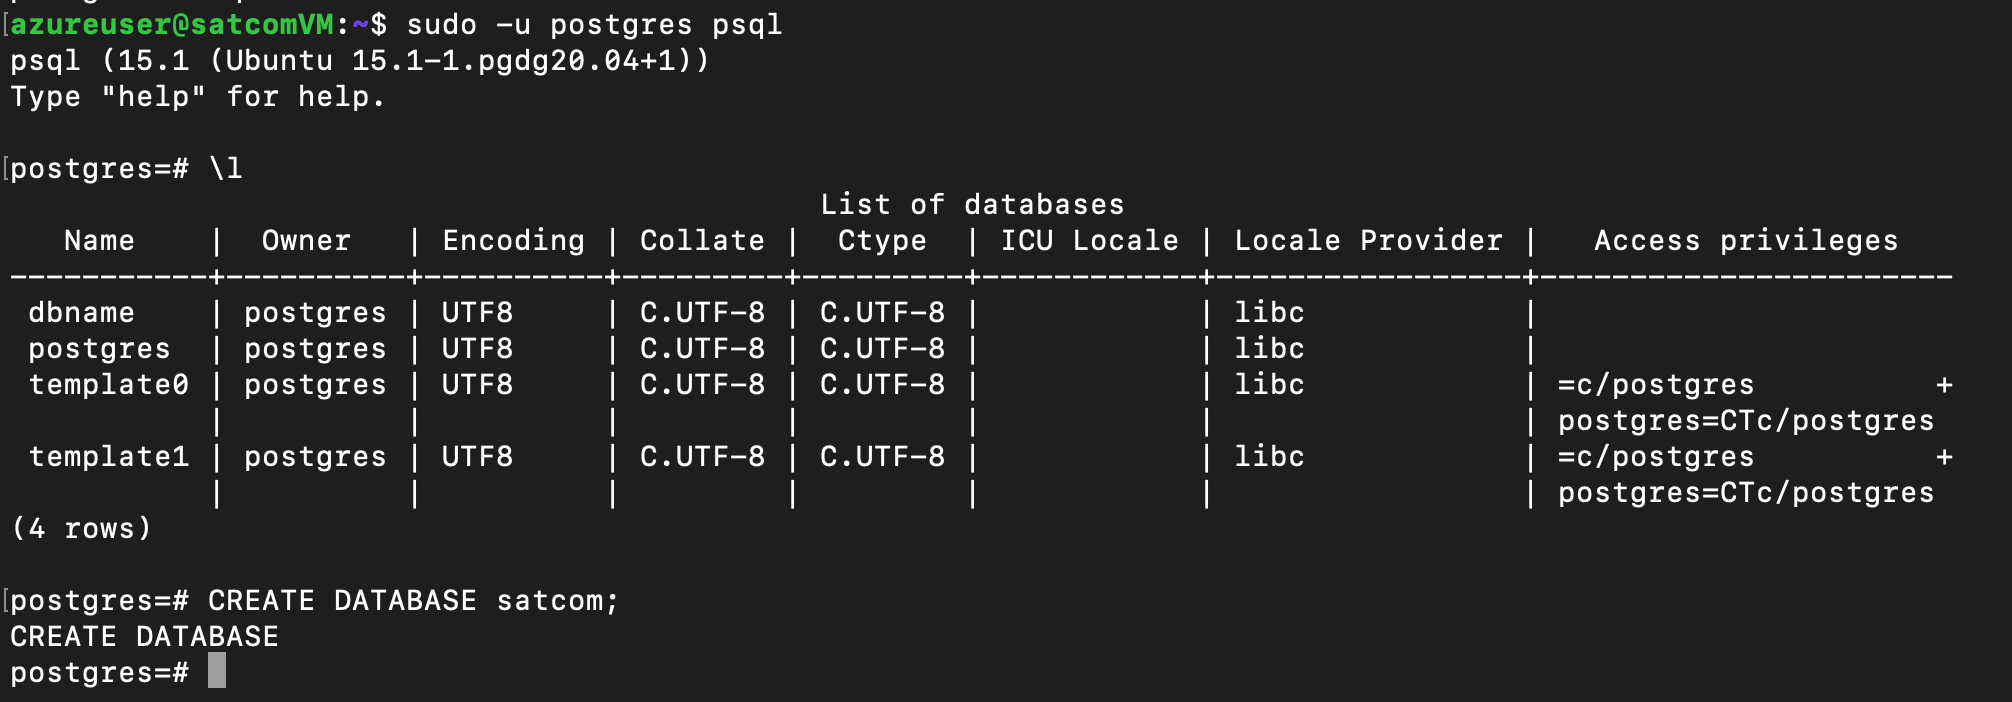
\includegraphics[width=\linewidth]{psql.png}
			\caption{Prikaz konfiguracije baze}
			\label{fig:baza}
		\end{figure}

		Kako bi backend dio aplikacije uspješno spremao i dohvaćao podatke potrebno je u prethodno instaliranoj Postgres bazi prije njegova pokretanja stvoriti bazu podataka pod nazivom 'satcom'. Za to je najjednostavnije koristiti defaultnog postgres korisnika koji dolazi s instalacijom postgres baze podataka te koristeći psql CLI generirati novu bazu podataka preko komandne linije. Ta baza podataka bit će popunjena podacima od strane aplikacije.
    \newline
      \begin{figure}[H]
			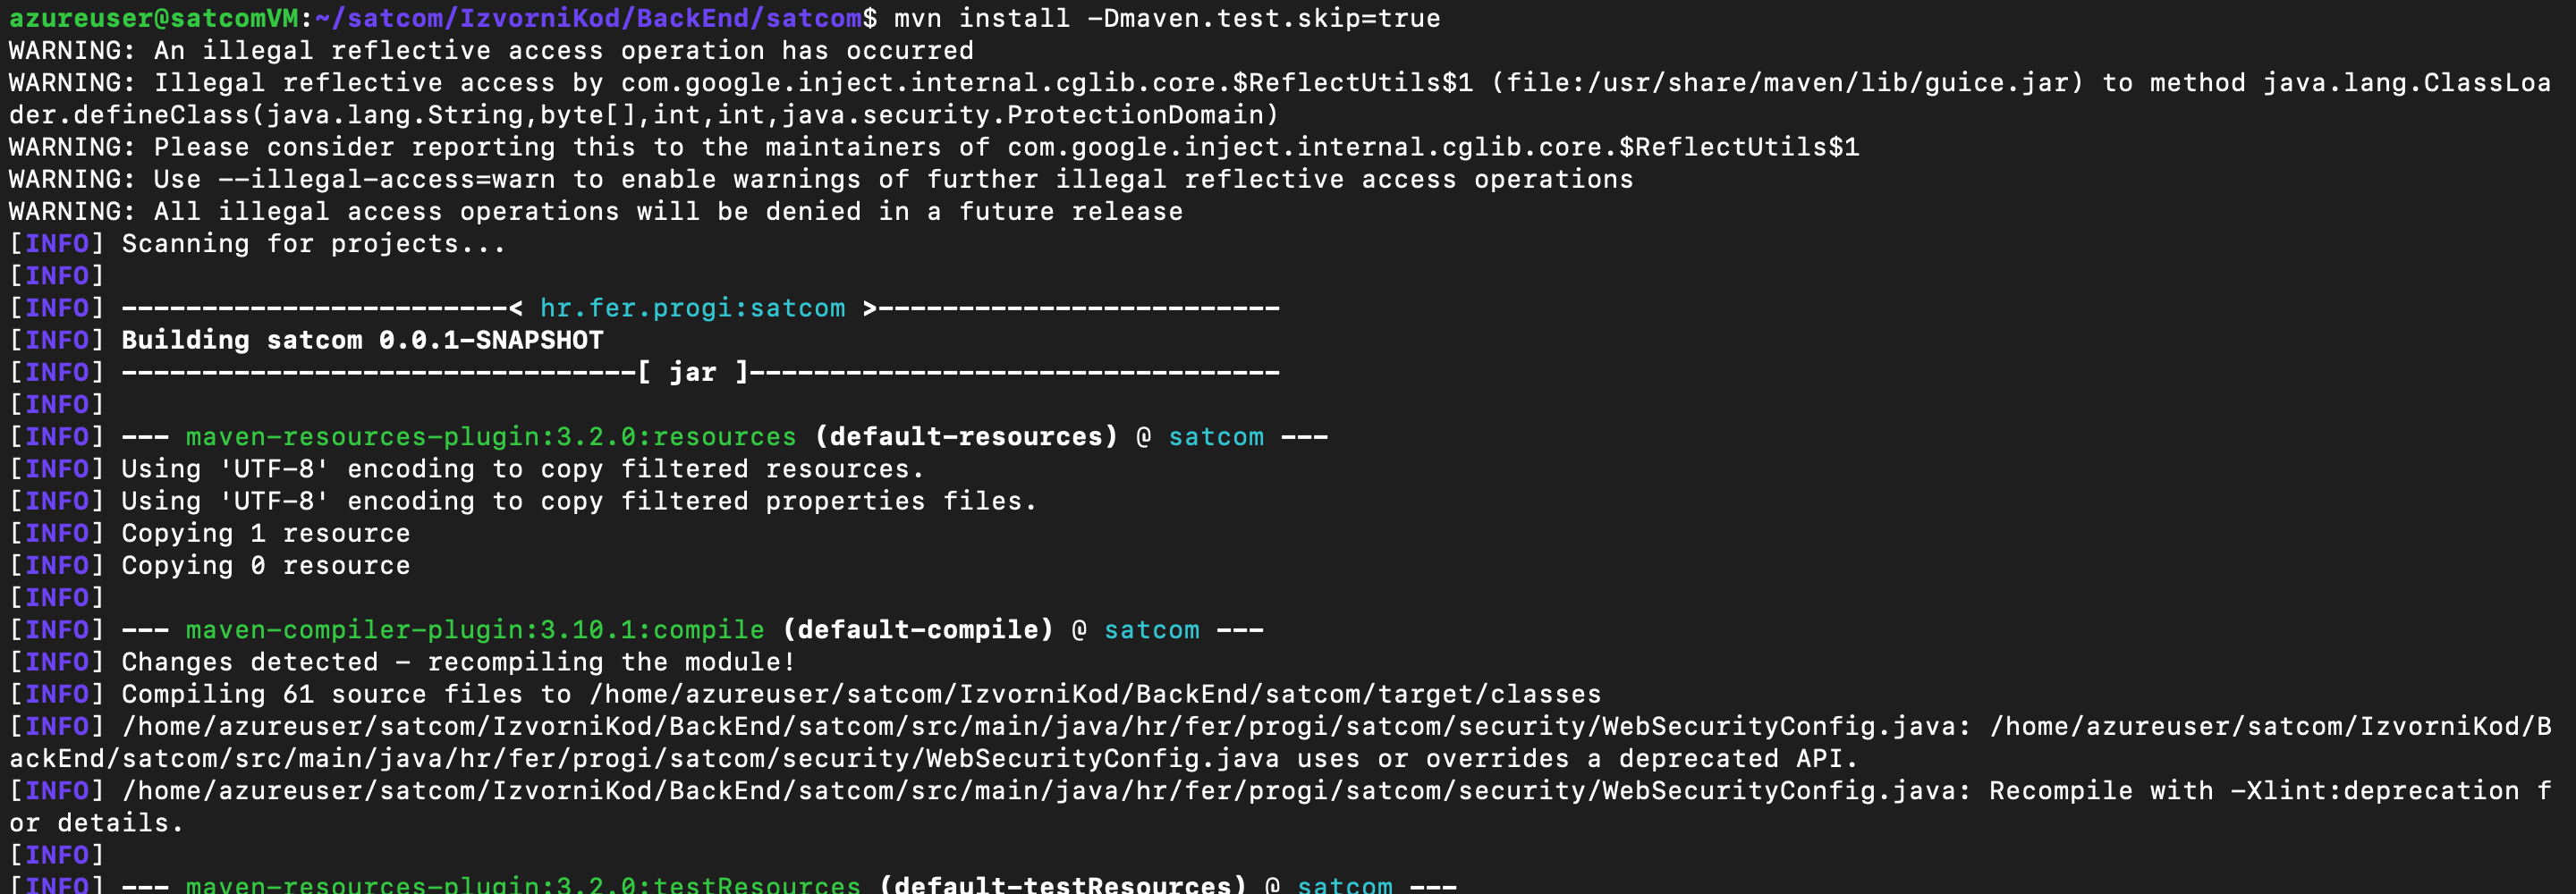
\includegraphics[width=\linewidth]{backend_mvn_install.png}
			\caption{Pokretanje maven builda}
			\label{fig:build}
		\end{figure}

    Za jednostavniji build backenda koristili smo Apache Maven project manager. Njega je također potrebno preuzeti kako bi se cjelokupna aplikacija uspješno izgradila prema postavkama definiranim unutar maven datoteke pom.xml. Ona definira određene ovisnosti (dependencies), build direktorij, izvorni direktorij, testni izvorni direktorij te ostale dodatke (plugins) koji su potrebni našoj aplikaciji da bi funkcionirala.
    \begin{figure}[H]
			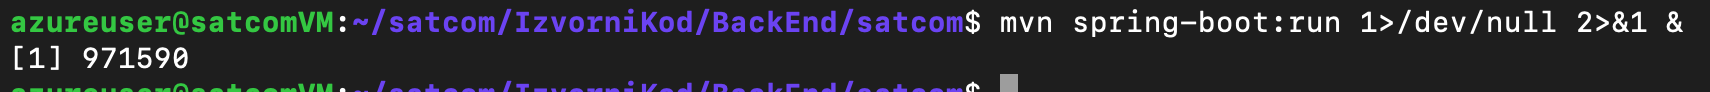
\includegraphics[width=\linewidth]{springboot_run.png}
			\caption{Pokretanje spring aplikacije}
			\label{fig:spring}
		\end{figure}
    

    \textbf{Konfiguracija frontenda}

		Za pokretanje frontend dijela aplikacije također je potrebno instalirati dodatnu programsku podršku. Prvotno je potrebno instalirati Node, također preko komandne linije, a zatim i npm koji služi kao package manager za Node aplikacije.
    \newline
    \newline
    
      \begin{figure}[H]
			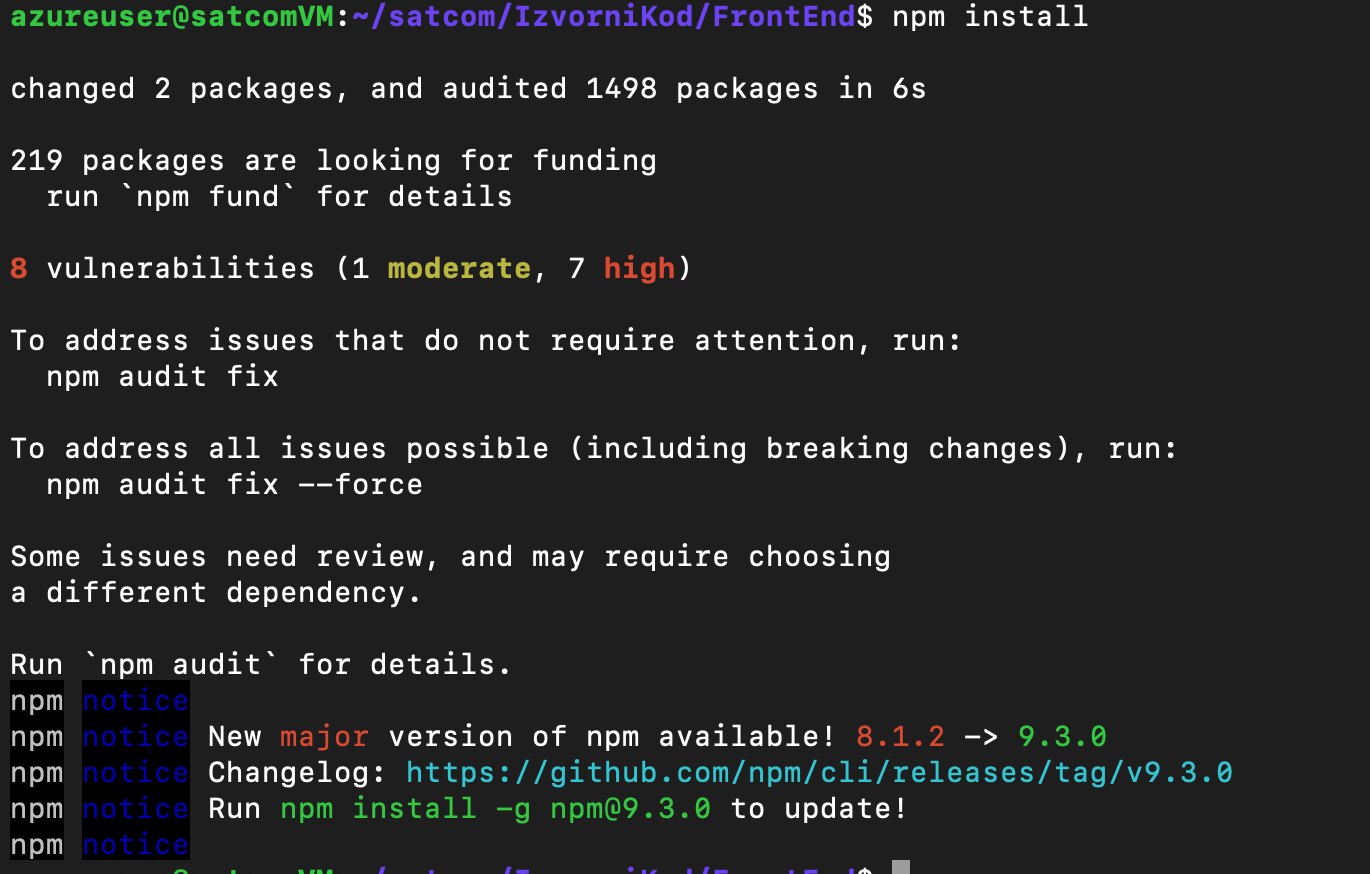
\includegraphics[width=\linewidth]{npm_install.png}
			\caption{Instaliranje node modula}
			\label{fig:npm}
		\end{figure}

    Nakon uspješno provedenih svih navedenih koraka potrebno je povući programski kod s odgovarajućeg git repozitorija.
    \begin{figure}[H]
			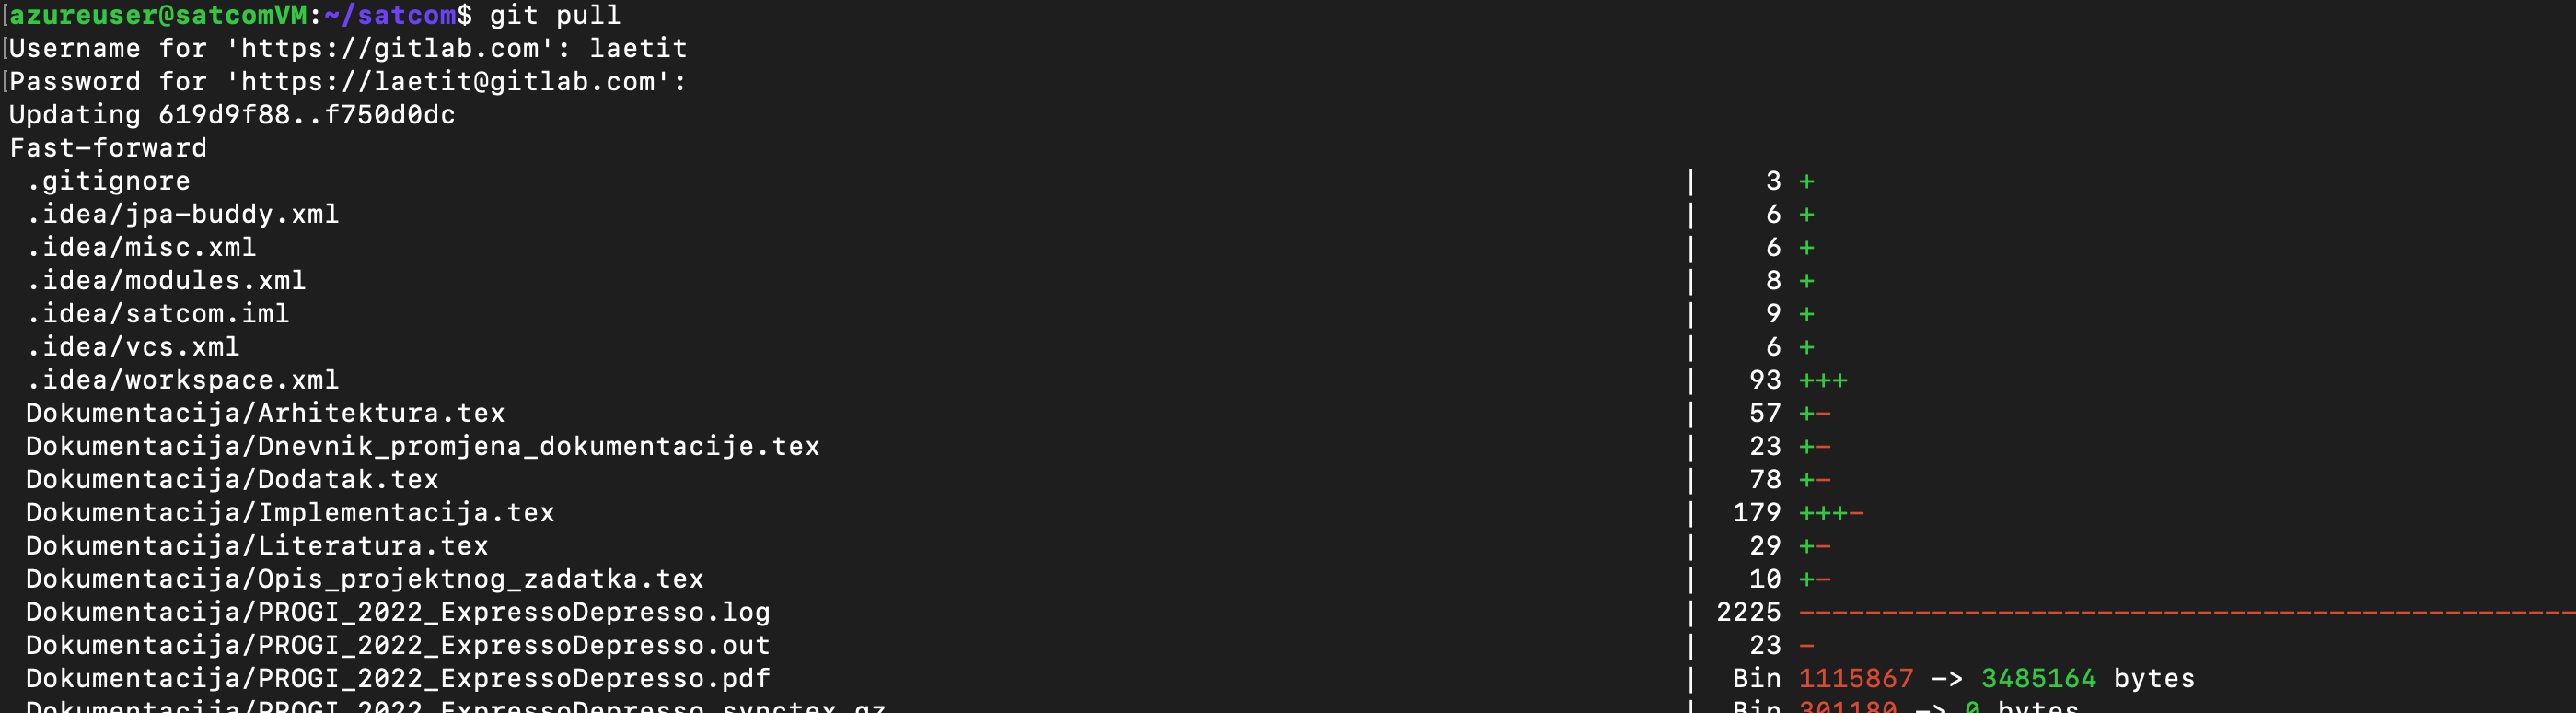
\includegraphics[width=\linewidth]{pull.png}
			\caption{Prikaz pullanja koda s gita}
			\label{fig:pull}
		\end{figure}
  Nakon uspješnog pulla imamo sve potrebne resurse za pokretanje aplikacije te je samo potrebno runnati maven projekte i node aplikaciju u odgovarajućim direktorijima na virtualnoj mašini. Poželjno je aplikaciju staviti da se vrti kao pozadinski proces na virtualnoj mašini.

			\eject 
	\chapter{Zaključak i budući rad}
		
		 Zadatak naše grupe bio je razvoj web aplikacije pod nazivom "SatCom". Ideja aplikacije je da se korisnicima omogući komunikacija sa satelitima u mreži SatNogs. Nakon 12 tjedana timskog rada, ostvarili smo zadani cilj i projekt je završen. Projekt je imao tri faze.\newline
		 Prva faza je uključivala okupljanje tima, razgovor o generalnim idejama za aplikaciju, izražavanje pojedinačnih interesa i želja za radom u prvom ciklusu predaje, te konačno podjela zadataka za prvi ciklus. Formirala su se dva podtima. U prvom podtimu članovi su radili na implementaciji funkcionalnosti na frontendu. U drugom podtimu su članovi su radili na implementaciji funkcionalnosti na backendu. Rad na dokumentaciji podijeljen je na više manjih zadataka koje su pojedinci samostalno preuzimali. Prva je faza projekta trajala do kolokviranja prvog ciklusa projekta.\newline
		 U drugoj je fazi naglasak bio na implementaciji aplikacije, te se i ovdje zadržala podjela u dva podtima koji su radili na programskom ostvarenju aplikacije. U ovoj je fazi dovršena implementacija aplikacije, a trajala je do demonstracije alfa inačice aplikacije.\newline
		 Treća i konačna faza je uključivala izradu raznih UML dijagrama, ispitivanje sustava, pronalazak i ispravak grešaka. U ovoj fazi također je zadržana podjela na dva podtima te su zadatke vezane uz dokumentaciju članovi tima preuzimali samostalno. Ova je faza trajala do završetka projekta, prije konačne predaje i kolokviranja drugog ciklusa.\newline
		 Izgrađenu aplikaciju je moguće proširiti na mnogo načina. Jedna od ideja je da se implementira stranica koja bi prikazivala geolokacije pojedinih stanica i informacije o njima poput uspješnosti u slanju poruka.
		 Sudjelovanje u ovom projektu je bilo vrijedno iskustvo za sve članove tima. Svima nama je ovo bio prvi ozbiljniji grupni projekt, i snašli smo se jako dobro. Konflikata u timu nije bilo, a suradnja i komunikacija su bili na iznimno zadovoljavajućoj razini. Većini nas je ovaj projekt bio prvi ozbiljniji dodir s tehnologijama poput Gita i Latex. Naučili smo koristiti neke moderne radne okvire pri izradi web aplikacija. Iznimno smo zadovoljni postignutim rezultatima i timskim radom koji je do tih rezultata doveo.



		
		\eject 
	\chapter*{Popis literature}
		\addcontentsline{toc}{chapter}{Popis literature}
		
		
		\begin{enumerate}
			
			
			\item  Programsko inženjerstvo, FER ZEMRIS, 
			 	\url{http://www.fer.hr/predmet/proinz}
			\item SatNOGS projekt, 
				\url {https://satnogs.org/about/}
			\item SatNOGS Network,  
				\url {https://network.satnogs.org/}
			\item SatNOGS Database, 
				 \url {https://db.satnogs.org/}
			\item SatNOGS Network API,
				\url {https://librespacefoundation.gitlab.io/-/satnogs/satnogs-network/-/jobs/3313398089/artifacts/satnogs-network-api-client/html2/index.html}
			
			\item  The Unified Modeling Language, \url{https://www.uml-diagrams.org/}
			
			\item  Astah Community, 
				\url{http://astah.net/editions/uml-new}
			\item BezKoder,
				\url {https://www.bezkoder.com/spring-boot-jwt-authentication/}
			\item  I. Sommerville, "Software engineering", 8th ed, Addison Wesley, 2007.
			\item Junit5 
				\url{https://junit.org/junit5/}
			\item Unit testiranje, Informacija, logika i jezici , FER ZTEL,
				\url{https://www.fer.unizg.hr/predmet/ilj_b}
			\item Java Networking,
				\url{https://docs.oracle.com/javase/8/docs/technotes/guides/net/index.html}
			\item Scheduling Tasks, Spring.io,
				\url{https://spring.io/guides/gs/scheduling-tasks/}
		\end{enumerate}
		
		 
	
	
	\begingroup
	\renewcommand*\listfigurename{Indeks slika i dijagrama}
	%\renewcommand*\listtablename{Indeks tablica}
	%\let\clearpage\relax
	\listoffigures
	%\vspace{10mm}
	%\listoftables
	\endgroup
	\addcontentsline{toc}{chapter}{Indeks slika i dijagrama}


	
	\eject 
		
	\chapter*{Dodatak: Prikaz aktivnosti grupe}
		\addcontentsline{toc}{chapter}{Dodatak: Prikaz aktivnosti grupe}
		%dd
		\section*{Dnevnik sastajanja}	
		\begin{packed_enum}
			\item  sastanak
			
			\item[] \begin{packed_item}
				\item Datum: 20.10.2022.
				\item Trajanje: 2h
			
			
				\item Prisustvovali: \begin{packed_enum}
				
				\item[]  M. C. Belušić Gonzales,
						 L. Crnković,
				  	     D. Grdić,
						 M. Pristav,
						 L. Salihović,
						 M. Vidas,
						 I. Žgela
				\end{packed_enum}
				\item Teme sastanka:
				\begin{packed_item}
					\item  Upoznavanje s zadatkaom
					\item  Izlučivanje zahtjeva aplikacije
					\item  Razriješavanje inicijalnih nedoumica
					\item  Odabir baznih tehnologija
					\item  Rasprava i opisivanje relacijskog modela baze podataka
					\item  Opisivanje osnovnog UI izgleda
					\item  Proučavanje API dokumentacije
				\end{packed_item}
			\end{packed_item}
		
		\item  sastanak
		
		\item[] \begin{packed_item}
			\item Datum: 25.10.2022.
			\item Trajanje: 3h
			
			
			\item Prisustvovali: \begin{packed_enum}
				
				\item[]  M. C. Belušić Gonzales,
				L. Crnković,
				D. Grdić,
				M. Pristav,
				L. Salihović,
				M. Vidas,
				I. Žgela
			\end{packed_enum}
			\item Teme sastanka:
			\begin{packed_item}
				\item  Upoznavanje s detaljima dokumentacije
				\item Započeta podjela posla oku dokumentacije
				\item Određeni načini praćenja rada u timu
			\end{packed_item}
		\end{packed_item}
	
		\item  sastanak
	
	\item[] \begin{packed_item}
		\item Datum: 26.10.2022.
		\item Trajanje: 1.5h
		
		
		\item Prisustvovali: \begin{packed_enum}
			
			\item[]  M. C. Belušić Gonzales,
			L. Salihović,
			I. Žgela
		\end{packed_enum}
		\item Teme sastanka:
		\begin{packed_item}
			\item  Definrian općenit dizaj i boje web stranice
			\item  Definirane komponente koje je potrebno implementirati
			\item Dogovor oko raspodjele poslova do slijedećeg sastanka
		\end{packed_item}
	\end{packed_item}
\item  sastanak

\item[] \begin{packed_item}
	\item Datum: 30.10.2022.
	\item Trajanje: 2.5h
	
	
	\item Prisustvovali: \begin{packed_enum}
		
		\item[]  L. Crnković,
		D. Grdić,
		M. Pristav,
		M. Vidas
	\end{packed_enum}
	\item Teme sastanka:
	\begin{packed_item}
		\item  Otrkriveni i prodiskutirani problemi sa spajanjem na API
		\item  Osvježen UML baze podataka
		\item  Istraživanje okolnosti našeg zadatka\newline (mogućnosti transmitera,antena,satelita...)
		\item  Istraživanje konkretnog formata potrebnih podataka
	\end{packed_item}
\end{packed_item}

\item  sastanak

\item[] \begin{packed_item}
	\item Datum: 31.10.2022.
	\item Trajanje: 1h
	
	
	\item Prisustvovali: \begin{packed_enum}
		
		\item[]  M. C. Belušić Gonzales,
		I. Žgela
		 
	\end{packed_enum}
	\item Teme sastanka:
	\begin{packed_item}
		\item  Zajedničko rješavanje konfilkata
		\item  Zajedničko rješavanje problema prijave korisnika u aplikaciju
		\item  Raspodjela zadataka i uređivnje gitlab board-a
		\item Međusobno pokazivanje koda i konzultacija za nastavak rada na aplikaciji
	\end{packed_item}
\end{packed_item}
\item  sastanak
\item[] \begin{packed_item}
	\item Datum: 2.11.2022.
	\item Trajanje: 3.5h
	
	
	\item Prisustvovali: \begin{packed_enum}
		
		\item[]  L. Crnković,
		D. Grdić,
		M. Pristav,
		M. Vidas
	\end{packed_enum}
	\item Teme sastanka:
	\begin{packed_item}
		\item  Testiranje get zahtjeva na API-ju
		\item  Planiranje daljnjeg rada backenda
		\item  Pojašnjenje novih aspekata dokumentacije
		\item  ispravljanje prijašnjih grešaka u radu i shvaćanju zadatka
		\item  Određen termin za zajedničko stvaranje dijela dokumentacija
	\end{packed_item}
\end{packed_item}

\item  sastanak

\item[] \begin{packed_item}
	\item Datum: 3.11.2022.
	\item Trajanje: 4h
	
	
	\item Prisustvovali: \begin{packed_enum}
		
		\item[]  
		L. Crnković,
		D. Grdić,
		M. Pristav,
		L. Salihović,
		M. Vidas,
		I. Žgela
	\end{packed_enum}
	\item Teme sastanka:
	\begin{packed_item}
		\item  Sastanak sa asistentom
		\item Provjera dosadašnjeg rada i uspunjenja zahtjeva zadatka
		\item Odlučen način i redovitost povezivanja na satnogs network
		\item Dovršen model baze podataka
		\item Napravljenji  dijagrami obrazaca uporabe
		\item Usklađivanje workspaceova na frontendu
		\item Dogovor oko načina predaje formi
	\end{packed_item}
\end{packed_item}
	\item  sastanak

\item[] \begin{packed_item}
	\item Datum: 10.11.2022.
	\item Trajanje: 4h
	
	
	\item Prisustvovali: \begin{packed_enum}
		
		\item[]  M. C. Belušić Gonzales,
		L. Crnković,
		D. Grdić,
		M. Pristav,
		L. Salihović,
		M. Vidas,
		I. Žgela
	\end{packed_enum}
	\item Teme sastanka:
	\begin{packed_item}
		\item  Usklađivanje frontend i backend ideja i dovršenog posla
		\item  Spajanje frontend i backend koda
		\item  Dovršavanje funkcionalnosti LogIn/LogOut
		\item  Dodavanje previđenih Obrazaca Uporabe
		\item  Zapoečta modelacija Sekvencijskih dijagrama
		\item  Zajednička provjera/pregled dijelova dokumentacije
		\item  Dodane manje preinake u bazu podataka
		\item  Raspravljene moguće promjene o finalnom načinu rada aplikacije
	\end{packed_item}
\end{packed_item}
	\item  sastanak
\item[] \begin{packed_item}
	\item Datum: 18.11.2022.
	\item Trajanje: 3h
	
	
	\item Prisustvovali: \begin{packed_enum}
		
		\item[] 
		L. Crnković,
		D. Grdić,	
		M. Vidas,
		I. Žgela
	\end{packed_enum}
	\item Teme sastanka:
	\begin{packed_item}
		\item Deployment aplikacije
		\item Testiranje deployane aplikacije
	\end{packed_item}
\end{packed_item}
%-------------------------------------------- novi sastanci
	\item  sastanak
\item[] \begin{packed_item}
	\item Datum: 19.12.2022.
	\item Trajanje: 4h
	
	
	\item Prisustvovali: \begin{packed_enum}
		
		\item[]  M. C. Belušić Gonzales,
		L. Crnković,
		D. Grdić,
		M. Pristav,
		L. Salihović,
		M. Vidas,
		I. Žgela
	\end{packed_enum}
	\item Teme sastanka:
	\begin{packed_item}
		\item Osvrt na demonstraciju alfa inačice
		\item Raspodjela preostale implementacije nakon sastanka s asistentom
		\item Postavljen rok za dovršetak implementacije i početak dokumentacije
		\item Dogovoren termin sljedećeg sastanka
		
	\end{packed_item}
\end{packed_item}
	\item  sastanak
\item[] \begin{packed_item}
	\item Datum: 5.1.2023.
	\item Trajanje: 2h
	
	
	\item Prisustvovali: \begin{packed_enum}
		
		\item[]  M. C. Belušić Gonzales,
		L. Crnković,
		D. Grdić,
		M. Pristav,
		L. Salihović,
		M. Vidas,
		I. Žgela
	\end{packed_enum}
	\item Teme sastanka:
	\begin{packed_item}
		\item Zajednički pregled funkcionalnosti aplikacije
		\item Pregled potrebnih znanja za daljnju dokumentaciju
		\item Raspodjela posla oko dokumentacije
		\item Predložene manje promjene u dizajnu aplikacije
		
		
	\end{packed_item}
\end{packed_item}



%

\end{packed_enum}

\eject
\section*{Tablica aktivnosti}

\begin{longtblr}[
label=none,
]{
	vlines,hlines,
	width = \textwidth,
	colspec={X[7, l]X[1, c]X[1, c]X[1, c]X[1, c]X[1, c]X[1, c]X[1, c]}, 
	vline{1} = {1}{text=\clap{}},
	hline{1} = {1}{text=\clap{}},
	rowhead = 1,
} 
\SetCell[c=1]{c}{} & 	\SetCell[c=1]{c}{\rotatebox{90}{\textbf{Mihael Pristav}}} & 	\SetCell[c=1]{c}{\rotatebox{90}{\textbf{Maria Carmen Belušić Gonzales }}} &		\SetCell[c=1]{c}{\rotatebox{90}{\textbf{Leticija Crnković}}} & 	\SetCell[c=1]{c}{\rotatebox{90}{\textbf{Dalen Grdić }}} &		\SetCell[c=1]{c}{\rotatebox{90}{\textbf{Leona Salihović }}} & 	\SetCell[c=1]{c}{\rotatebox{90}{\textbf{Marta Vidas }}} &		\SetCell[c=1]{c}{\rotatebox{90}{\textbf{Ivan Žgela }}} \\  
Opis projektnog zadatka 	& 1 &5  &  &  &  &  & \\ 

Funkcionalni zahtjevi       &1  &  &  & & 2 &0.5  &  \\ 
Opis pojedinih obrazaca 	&11  &  &  &  & 2.5 &2  & 0.5 \\ 
Dijagram obrazaca 			&1.5  &  &  &  &  & &  \\
Sekvencijski dijagrami 		&1  &  &  &  &  &  &  \\ 
Opis ostalih zahtjeva 		&  &  &  &  &  &0.5  &  \\ 

Arhitektura i dizajn sustava	 &  &  &  &  &  &0.5 &  \\ 
Baza podataka				&2  &  &  &  &  & 4.5 & 2.5  \\ 
Dijagram razreda 			&  &  &1.5  &  &  &0.5  &   \\ 
Dijagram stanja				&  &  &  &  &  &  &2  \\ 
Dijagram aktivnosti 		&  &  &1  &1  &  &  &  \\ 
Dijagram komponenti			&  &  &  & 1 &  &1  &  \\ 
Korištene tehnologije i alati 		&0.5  &  &  &  &2  &  &  \\ 
Ispitivanje programskog rješenja 	&1  &2.5  &  &  &  &1  &  \\ 
Dijagram razmještaja			&  &  &  &  &1  &  &  \\ 
Upute za puštanje u pogon 		&  &  &4  &  &  &  &  \\  
Dnevnik sastajanja 			&2  &  &  &  &  &  &0.5  \\ 
Zaključak i budući rad 		&  &  &  &  &2  &  &  \\  
Popis literature 			&1  &  &  &  &  &  &  \\  
\textbf{Ukupno dokumentacija}	&22  &7.5  &6.5  &2  &9.5  & 10.5 &5.5  \\ 
 
\textit{Upravljanje projektom} 		& 11 &  &  &  &  &  & \\
\textit{back end} 							&24  &  &17  &30  &  &36  &  \\  
\textit{front end} 							&  &28  &  &  & 22 &  & 42 \\  

\textit{deployment} 							&  &4  &17  &15  &5  &10  &3  \\
\textit{Istraživanje informacija/tehnologija} 				&10  &12  &7.5  &7.5  &10  &6.5  &11 
\\
%tu sam odlučilpisati kolko vremena je otišlo napodešavanje-/popravljanje te njihove blesave skripte u latecu + proucavanje materjala za dokumentaciju iskreno nisam znal kad drugdje to zapisat
\textit{izrada baze podataka} 		 			&2  &  &1  &1  &  &1  & \\ 
\textit{izrada dijagrama} 		 			&10  & 3.5 &8  &11.5  &3  &7  &4 \\ 
\textit{izrada dizajna aplikacije u Figmi} 		 			&  &  &  &  & 6 &  & \\

\textbf{Ukupno razvoj projekta}	&79  &55 &57 &67 &55.5 &71 & 65.5 \\\end{longtblr}
					
					
		\eject
		\section*{Dijagrami pregleda promjena}
		
		 \begin{figure}[H]
			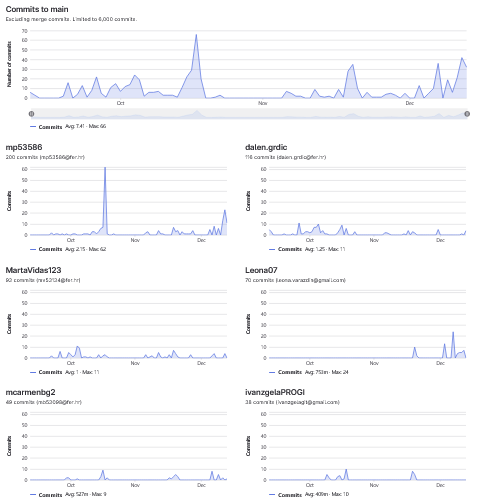
\includegraphics[width=\linewidth]{grafComitova.png}
			\caption{Graf gitLab aktivnosti}
			\label{fig:DijagramGitlaba}
		\end{figure}
	\begin{figure}[H]
		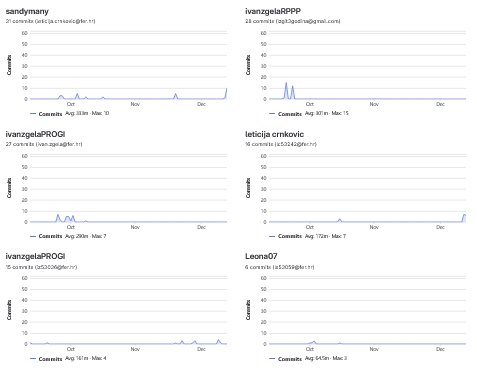
\includegraphics[width=\linewidth]{grafComitova2.png}
		\caption{Graf gitLab aktivnosti-nastavak}
		\label{fig:DijagramGitlaba2}
	\end{figure}
		
	



\end{document} %naredbe i tekst nakon ove naredbe ne ulaze u izgrađen dokument 


